\setcounter{chapter}{2}
\chapter{零温单粒子格林函数, 费曼图技术及其应用}
\begin{introduction}
\item 零温单粒子格林函数
\item 物理量的表示
\item 零温单粒子格林函数的相互作用绘景
\item Wick 定理
\item 坐标空间单粒子格林函数的费曼图技术
\item 动量空间单粒子格林函数的费曼图技术
\item Dyson 方程
\item 费曼图技术在凝胶模型中的应用
\end{introduction}
\section{零温单粒子格林函数}
薛定谔绘景中引入场算符 $\hat{\psi}_{\sigma}(\boldsymbol{r})$ 和 $\hat{\psi}_{\sigma}^{\dagger}(\boldsymbol{r})$, 表示在空间某点 $\boldsymbol{r}$ 湮灭或产生一个自旋为 $\sigma$ 的粒子, 可以在一组正交完备基 $\left\{\phi_{k}(\boldsymbol{r})\right\}$ (注意这里 $k$ 是表征完备基的量子数)下展开:
\begin{equation}
\left\{\begin{aligned}
\hat{\psi}_{\sigma}(\boldsymbol{r}) \equiv \sum_{k} \phi_{k}(\boldsymbol{r}) \hat{C}_{k \sigma}, \\
\hat{\psi}_{\sigma}^{\dagger}(\boldsymbol{r}) \equiv \sum_{k} \phi_{k}^*(\boldsymbol{r}) \hat{C}_{k \sigma}^{\dagger}.
\end{aligned}\right.
\end{equation}
这里只考虑正常态, 不包括超导态、玻色-爱因斯坦凝聚态等复杂状态. 完备基的选择视具体情况而定, 通常可以选择平面波表象、布洛赫表象和瓦尼尔表象, $\hat{C}_{k \sigma}^{\dagger}$ 和 $\hat{C}^{}_{k \sigma}$ 则是相应表象下的产生和湮灭算符. 

选择布洛赫表象时, 体系有多条能带, 对于费米子通常选择最靠近费米面的能带. 需要强调的是 $\left\{\phi_{k}(\boldsymbol{r})\right\}$ 是全同粒子体系中单体算符的正交完备基，这样的全同粒子体系可能是由实物粒子如电子等组成, 也可能是由非实物粒子如声子等元激发组成. 具体表象下产生湮灭算符间有如下对易关系:
\begin{equation}
\left[\hat{C}^{}_{k \sigma}, \hat{C}_{k^{\prime} \sigma^{\prime}}^{\dagger}\right]_{\mp}=\delta_{k k^{\prime}} \delta_{\sigma \sigma^{\prime}}, \quad\left[\hat{C}_{k \sigma}, \hat{C}_{k^{\prime} \sigma^{\prime}}\right]_{\mp}=\left[\hat{C}_{k \sigma}^{\dagger}, \hat{C}_{k^{\prime} \sigma^{\prime}}^{\dagger}\right]_{\mp}=0,
\end{equation}
其中 $-$ 表示玻色子算符间的对易关系, $+$ 表示费米子的反对易关系. 这里和之后将这两种关系写在一起，代表玻色子的符号在上，代表费米子的符号在下. 利用这些关系和基底间的正交完备性可以得到场算符间的对易关系:
\begin{equation}
\left[\hat{\psi}^{}_{\sigma}(\boldsymbol{x}), \hat{\psi}_{\sigma^{\prime}}^{\dagger}\left(\boldsymbol{x}^{\prime}\right)\right]_{\mp}=\delta\left(\boldsymbol{x}-\boldsymbol{x}^{\prime}\right) \delta_{\sigma \sigma^{\prime}}, 
\end{equation}
\begin{equation}
\left[\hat{\psi}_{\sigma}(\boldsymbol{x}), \hat{\psi}_{\sigma^{\prime}}\left(\boldsymbol{x}^{\prime}\right)\right]_{\mp}=\left[\hat{\psi}_{\sigma}^{\dagger}(\boldsymbol{x}), \hat{\psi}_{\sigma^{\prime}}^{\dagger}\left(\boldsymbol{x}^{\prime}\right)\right]_{\mp}=0 .
\end{equation}
利用海森伯绘景和薛定谔绘景中算符的变换关系, 可以得到海森伯绘景下场算符 $\hat{\psi}_{H \sigma}(\boldsymbol{x}, t)$ 与薛定谔绘景下场算符 $\hat{\psi}_{\sigma}(\boldsymbol{x})$ 的关系:
\begin{equation}
\hat{\psi}_{H \sigma}(\boldsymbol{x}, t)=\mathrm{e}^{\mathrm{i} \hat{H} t} \hat{\psi}_{\sigma}(\boldsymbol{x}) \mathrm{e}^{-\mathrm{i} \hat{H} t},
\end{equation}
这里的哈密顿量不显含时间.

\subsection{零温单粒子格林函数的定义}
\begin{definition}{零温单粒子格林函数}{}
\begin{equation}
G_{\alpha \beta}\left(\boldsymbol{x}, t ; \boldsymbol{x}^{\prime}, t^{\prime}\right) \equiv-\mathrm{i}\left\langle\psi_{H}^{0}\left|\hat{T}\left[\hat{\psi}^{}_{H \alpha}(\boldsymbol{x}, t) \hat{\psi}_{H \beta}^{\dagger}\left(\boldsymbol{x}^{\prime}, t^{\prime}\right)\right]\right| \psi_{H}^{0}\right\rangle .
\end{equation}
\end{definition}
\begin{note}
    格林函数的极点是粒子的能量, 亦即哈密顿量的本征值. 一般来说本征值是实数. 但由于现在产生的是准粒子, 准粒子在运动过程中由于与其他粒子的相互作用, 可能会衰变.
    所以准粒子是有寿命的, 这一点在格林函数上表示为极点是个复数. 实部表示准粒子的能量, 虚部的倒数是准粒子的寿命. 当粒子不衰变时, 虚部是无穷小量, 寿命无限长. 
    
    这里的 $\left| \psi_H^0 \rrag$ 与我们之前定义的 $\left| E_g \rrag$ 同为基态, 这样表示是为了
    强调式中所有物理量都在海森伯绘景中.
\end{note}
$\left|\psi_{H}^{0}\right\rangle$ 的本征值方程是
\begin{equation}
\hat{H}\left|\psi_{H}^{0}\right\rangle=E_{g}\left|\psi_{H}^{0}\right\rangle .
\end{equation}

引入编时算符 $\hat{T}$, 定义为
\begin{align}
\hat{T}\left[\hat{A}_{H}(t) \hat{B}_{H}\left(t^{\prime}\right)\right]&=\left\{\begin{aligned}
&\hat{A}_{H}(t) \hat{B}_{H}\left(t^{\prime}\right), &t>t^{\prime}, \\
&\pm \hat{B}_{H}\left(t^{\prime}\right) \hat{A}_{H}(t), &t<t^{\prime}
\end{aligned}\right. \nonumber\\
&=\theta(t-t^\prime)\hat{A}_{H}(t) \hat{B}_{H}\left(t^{\prime}\right)\pm\theta(t^\prime-t)\hat{B}_{H}\left(t^{\prime} \right)\hat{A}_{H}(t),
\end{align}
且有
\begin{equation}
\hat{T}\left[\hat{A}(t) \hat{B}\left(t^{\prime}\right)\right]=\hat{T}\left[\pm \hat{B}\left(t^{\prime}\right) \hat{A}(t)\right].
\end{equation}

\subsection{对称性质}
零温单粒子格林函数在有对称性的体系下, 形式可以简化, 具体体现在其所依赖的参量减少:
\begin{enumerate}
\item $\hat{H}$ 不显含时间, 具有时间对称性
\begin{equation}
G_{\alpha \beta}\left(\boldsymbol{x}, t ; \boldsymbol{x}^{\prime}, t^{\prime}\right)=G_{\alpha \beta}\left(\boldsymbol{x}, \boldsymbol{x}^{\prime} ; t-t^{\prime}\right) .
\end{equation}
\item 空间均匀 $([\hat{H}, \hat{P}]_-=0)$, 具有平移对称性
\begin{equation}
G_{\alpha \beta}\left(\boldsymbol{x}, t ; \boldsymbol{x}^{\prime}, t^{\prime}\right)=G_{\alpha \beta}\left(\boldsymbol{x}-\boldsymbol{x}^{\prime} ; t, t^{\prime}\right) .
\end{equation}
\item 相互作用与自旋无关
\begin{equation}
G_{\alpha \beta}\left(\boldsymbol{x}, t ; \boldsymbol{x}^{\prime}, t^{\prime}\right)=G\left(\boldsymbol{x}, t ; \boldsymbol{x}^{\prime}, t^{\prime}\right) \delta_{\alpha \beta} ,
\end{equation}
其中
\begin{equation}
G\left(\boldsymbol{x}, t ; \boldsymbol{x}^{\prime}, t^{\prime}\right)\equiv\frac{\displaystyle\sum_\alpha G_{\alpha \alpha}\left(\boldsymbol{x}, t ; \boldsymbol{x}^{\prime}, t^{\prime}\right)}{\displaystyle\sum_\alpha 1}=\frac{\displaystyle\sum_\alpha G_{\alpha \alpha}\left(\boldsymbol{x}, t ; \boldsymbol{x}^{\prime}, t^{\prime}\right)}{2S+1}.
\end{equation}
\item 具备以上三个对称性
\begin{equation}
G_{\alpha \beta}\left(\boldsymbol{x}, t ; \boldsymbol{x}^{\prime}, t^{\prime}\right)=G\left(\boldsymbol{x}-\boldsymbol{x}^{\prime} ; t-t^{\prime}\right)\delta_{\alpha \beta }.
\end{equation}
\end{enumerate}

\subsection{物理意义}
假设 $t>t^{\prime}$, 将场算符化为在薛定谔绘景下的表示:
\begin{align}
G_{\alpha \beta}\left(\boldsymbol{x}, t ; \boldsymbol{x}^{\prime}, t^{\prime}\right) &=-\mathrm{i}\left\langle\psi_{H}^{0}\left|\hat{\psi}^{}_{H \alpha}(\boldsymbol{x}, t) \hat{\psi}_{H \beta}^{\dagger}\left(\boldsymbol{x}^{\prime}, t^{\prime}\right)\right| \psi_{H}^{0}\right\rangle \nonumber\\
&=-\mathrm{i}\left\langle\psi_{H}^{0}\left|\mathrm{e}^{\mathrm{i} \hat{H} t}\hat{\psi}^{}_{\alpha}(\boldsymbol{x})\mathrm{e}^{-\mathrm{i} \hat{H} t}\mathrm{e}^{\mathrm{i} \hat{H} t^{\prime}} \hat{\psi}_{\beta}^{\dagger}\left(\boldsymbol{x}^{\prime}\right)\mathrm{e}^{-\mathrm{i} \hat{H} t^{\prime}}\right| \psi_{H}^{0}\right\rangle\nonumber\\
&=-\mathrm{i} \mathrm{e}^{\mathrm{i} E_{g}\left(t-t^{\prime}\right)}\left\langle\psi_{H}^{0}\left|\hat{\psi}^{}_{\alpha}(\boldsymbol{x}) \mathrm{e}^{-\mathrm{i}\hat{H}\left(t-t^{\prime}\right)} \hat{\psi}_{\beta}^{\dagger}\left(\boldsymbol{x}^{\prime}\right)\right| \psi_{H}^{0}\right\rangle .
\end{align}
这样, 零温单粒子格林函数的物理意义便是: $t^{\prime}$ 时刻基态中 $\boldsymbol{x}^{\prime}$ 位置产生一个自旋为 $\beta$ 的粒子, 然后经过 $t-t^{\prime}$ 的演化在 $t$ 时刻这一粒子在 $\boldsymbol{x}$ 处且自旋为 $\alpha$ 消灭的几率幅.

\section{物理量的表示}
\subsection{单体算符的基态平均}
单体算符可以利用场算符写为(二次量子化):
\begin{equation}
\hat{F}^{(1)}=\sum_{\alpha \beta} \int \hat{\psi}_{\alpha}^{\dagger}(\boldsymbol{x}) \hat{f}^{}_{\alpha \beta}(\boldsymbol{x}) \hat{\psi}^{}_{\beta}(\boldsymbol{x}) \mathrm{d} \boldsymbol{x} ,
\end{equation}
其在(零温)基态下的均值为:
\begin{align}
\left\langle\psi_{H}^{0}\left|\hat{F}^{(1)}\right| \psi_{H}^{0}\right\rangle &=\sum_{\alpha \beta} \int \mathrm{d} \boldsymbol{x}\left\langle\psi_{H}^{0}\left|\hat{\psi}_{\alpha}^{\dagger}(\boldsymbol{x}) \hat{f}^{}_{\alpha \beta}(\boldsymbol{x}) \hat{\psi}^{}_{\beta}(\boldsymbol{x})\right| \psi_{H}^{0}\right\rangle\nonumber \\
&=\sum_{\alpha \beta} \int \mathrm{d} \boldsymbol{x} \lim _{\boldsymbol{x}^{\prime} \rightarrow \boldsymbol{x}} \hat{f}_{\alpha \beta}(\boldsymbol{x})\left\langle\psi_{H}^{0}\left|\hat{\psi}_{\alpha}^{\dagger}\left(\boldsymbol{x}^{\prime}\right) \hat{\psi}^{}_{\beta}(\boldsymbol{x})\right| \psi_{H}^{0}\right\rangle ,
\end{align}
注意这里 $\hat{f}_{\alpha \beta}(\boldsymbol{x})$ 只作用在后面与 $\boldsymbol{x}$ 有关的项，所以上面的等式是成立的. 进一步, 写成海森伯绘景中的形式:
\begin{align}
&\left\langle\psi_{H}^{0}\left|\hat{F}^{(1)}\right| \psi_{H}^{0}\right\rangle\nonumber\\
=&\sum_{\alpha \beta} \int \mathrm{d} \boldsymbol{x} \lim _{\boldsymbol{x}^{\prime} \rightarrow \boldsymbol{x}} \hat{f}_{\alpha \beta}(\boldsymbol{x})\left\langle\psi_{H}^{0}\left| \mathrm{e}^{-\mathrm{i} \hat{H} t} \hat{\psi}_{H \alpha}^{\dagger}\left(\boldsymbol{x}^{\prime},t\right)\mathrm{e}^{\mathrm{i} \hat{H} t} \mathrm{e}^{-\mathrm{i} \hat{H} t} \hat{\psi}^{}_{H \beta}(\boldsymbol{x},t) \mathrm{e}^{\mathrm{i} \hat{H} t} \right| \psi_{H}^{0}\right\rangle\nonumber\\
=&\sum_{\alpha \beta} \int \mathrm{d} \boldsymbol{x} \lim _{\boldsymbol{x}^{\prime} \rightarrow \boldsymbol{x}} \hat{f}_{\alpha \beta}(\boldsymbol{x})\left\langle\psi_{H}^{0}\left|\hat{\psi}_{H \alpha}^{\dagger}\left(\boldsymbol{x}^{\prime}, t\right) \hat{\psi}^{}_{H \beta}(\boldsymbol{x}, t)\right| \psi_{H}^{0}\right\rangle .
\end{align}
为了与单粒子零温格林函数联系, 可以引入时间的极限:
\begin{align}
&\left\langle\psi_{H}^{0}\left|\hat{F}^{(1)}\right| \psi_{H}^{0}\right\rangle \nonumber\\
=&\sum_{\alpha \beta} \int \mathrm{d} \boldsymbol{x} \lim_{t'\to t^+\atop\vct{x}'\to \vct{x}}  \hat{f}_{\alpha \beta}(\boldsymbol{x})\left\langle\psi_{H}^{0}\left|\hat{\psi}_{H \alpha}^{\dagger}\left(\boldsymbol{x}^{\prime}, t^{\prime}\right) \hat{\psi}^{}_{H \beta}(\boldsymbol{x}, t)\right| \psi_{H}^{0}\right\rangle \nonumber\\
=&\sum_{\alpha \beta} \int \mathrm{d} \boldsymbol{x} \lim_{t'\to t^+\atop\vct{x}'\to \vct{x}}  \hat{f}_{\alpha \beta}(\boldsymbol{x})\left\langle\psi_{H}^{0}\left|\hat{T}\left[\hat{\psi}_{H \alpha}^{\dagger}\left(\boldsymbol{x}^{\prime}, t^{\prime}\right) \hat{\psi}^{}_{H \beta}(\boldsymbol{x}, t)\right]\right| \psi_{H}^{0}\right\rangle \nonumber\\
=&\pm \sum_{\alpha \beta} \int \mathrm{d} \boldsymbol{x} \lim_{t'\to t^+\atop\vct{x}'\to \vct{x}} \hat{f}_{\alpha \beta}(\boldsymbol{x})\left\langle\psi_{H}^{0}\left|\hat{T}\left[\hat{\psi}^{}_{H \beta}(\boldsymbol{x}, t) \hat{\psi}_{H \alpha}^{\dagger}\left(\boldsymbol{x}^{\prime}, t^{\prime}\right)\right]\right| \psi_{H}^{0}\right\rangle \nonumber\\
=&\pm \mathrm{i} \sum_{\alpha \beta} \int \mathrm{d} \boldsymbol{x} \lim_{t'\to t^+\atop\vct{x}'\to \vct{x}}  \hat{f}_{\alpha \beta}(\boldsymbol{x}) G_{\beta \alpha}\left(\boldsymbol{x}, t ; \boldsymbol{x}^{\prime}, t^{\prime}\right) .
\end{align}

\begin{example}
\textbf{总动能算符的基态平均.}

总动能算符是单体算符, 可以写为:
\begin{equation}
\hat{T}_{K}=\sum_{\alpha} \int \hat{\psi}_{\alpha}^{\dagger}(\boldsymbol{x})\left(-\frac{\nabla^{2}}{2 m}\right) \hat{\psi}^{}_{\alpha}(\boldsymbol{x}) \mathrm{d} \boldsymbol{x},
\end{equation}
这里暗含:
\begin{equation}
\hat{f}_{\alpha \beta}(\boldsymbol{x})=-\frac{\nabla^{2}}{2 m} \delta_{\alpha \beta} .
\end{equation}
总动能算符的基态平均为:
\begin{align}
\left\langle\psi_{H}^{0}\left|\hat{T}_{K}\right| \psi_{H}^{0}\right\rangle&=\pm \mathrm{i} \sum_{\alpha\beta} \int \mathrm{d} \boldsymbol{x} \lim_{t'\to t^+\atop\vct{x}'\to \vct{x}}  \left(-\frac{\nabla^{2}}{2 m}\delta_{\alpha \beta}\right) G_{\beta \alpha}\left(\boldsymbol{x}, t ; \boldsymbol{x}^{\prime}, t^{\prime}\right)\nonumber\\
&=\pm \mathrm{i} \sum_{\alpha} \int \mathrm{d} \boldsymbol{x} \lim_{t'\to t^+\atop\vct{x}'\to \vct{x}} \left(-\frac{\nabla^{2}}{2 m}\right) G_{\alpha \alpha}\left(\boldsymbol{x}, t ; \boldsymbol{x}^{\prime}, t^{\prime}\right).
\end{align}
\end{example}

\subsection{基态能(两种方法求解)}
(i) \textbf{方法之一}

全同费米子体系的哈密顿量是
\begin{equation}
    \hat{H}=\hat{T}_{K}+\hat{V},
\end{equation}
其中动能项和势能项分别为
   \begin{align}
        \hat{T}_{K}&=\sum_{\sigma}\int\dd\vct{x}\hat{\psi}_\sigma^\dg(\vct{x})\ls -\frac{\nabla^2}{2m} \rs \hat{\psi}_\sigma(\vct{x}),\\
        \hat{V}&=\frac{1}{2}\sum_\alpha\sum_\beta\iint\dd\vct{x}\dd\vct{x}'\hat{\psi}_\alpha^\dg(\vct{x})\psi_\beta^\dg(\vct{x}')\hat{V}(|\vct{x}-\vct{x}'|)\hat{\psi}_{\beta}^{ }(\vct{x}')\hat{\psi}_\alpha^{ }(\vct{x}).
    \end{align}
于是系统的基态能可以表示为
\begin{equation}
    E_g=\llag \psi_H^0\left|\hat{H}\right|\psi_H^0 \rrag=\llag \psi_H^0\left|\hat{T}_k\right|\psi_H^0 \rrag+\llag\psi_H^0\left| \hat{V} \right| \psi_H^0 \rrag,
\end{equation}
其中动能项的基态平均是
\begin{equation}
    \llag \psi_H^0 \left| \hat{T}_{K} \right| \psi_H^0\rrag=-\ii\sum_\sigma\int\dd\vct{x}\lim_{t'\to t^+\atop\vct{x}'\to \vct{x}}\ls -\frac{\nabla^2}{2m} \rs G_{\sigma\sigma}(\vct{x},t;\vct{x}',t'),
\end{equation}
但是势能项的基态平均 $\llag \psi_H^0 \left| \hat{V} \right|\psi_H^0\rrag$ 需要详细计算. 下面利用运动方程求解.

场算符的海森伯运动方程是
\begin{equation}
    \ii\frac{\pt}{\pt t}\hat{\psi}_{H\alpha}(\vct{x},t)=\lmi \hat\psi_{H\alpha}(\vct{x},t),\hat{H} \rmi_-,
\end{equation}
其中右式需要先换到薛定谔绘景下求解对易子, 再通过时间演化算符换回含时的形式, 即
\begin{equation}
    \lmi \hat{\psi}_{H\alpha},\hat{H} \rmi_-=\e^{\ii\hat{H}t}\lmi \hat{\psi}_\alpha(\vct{x}),\hat{H} \rmi_-\e^{-\ii\hat{H}t},
\end{equation}
其中右边的对易式可以写成:
\begin{equation}\label{329}
    \lmi \hat\psi^{ }_\alpha(\vct{x}),\hat{H} \rmi_-=\ls -\frac{\nabla^2}{2m} \rs\hat{\psi}^{ }_\alpha(\vct{x})+\sum_\sigma\int\dd\vct{z}' \hat{\psi}_\sigma^\dg(\vct{z}') \hat{V}(\vct{x},\vct{z}')\hat{\psi}^{ }_\sigma(\vct{z'})\hat{\psi}^{ }_\alpha(\vct{x}).
\end{equation}
\begin{question}{}{}
证明式\eqref{329}成立.
\end{question}
代回运动方程, 得到
\begin{equation}
    \ls \ii\frac{\pt}{\pt t}+\frac{\nabla^2}{2m} \rs\hat\psi_{H\alpha}(\vct{x},t)=\sum_\sigma\int\dd\vct{z}'\hat\psi_{H\sigma}^\dg(\vct{z}',t)\hat{V}(\vct{x},\vct{z}')\hat\psi_{H\sigma}(\vct{z}',t)\hat\psi_{H\alpha}(\vct{x},t).
\end{equation}
对等式两边左乘 $\hat\psi_{H\alpha}^\dg(\vct{x}',t')$ 然后取基态平均, 得到
  \begin{align}
        &\llag \psi_H^0\left| \hat\psi_{H\alpha}^\dg(\vct{x}',t')\ls \ii\frac{\pt}{\pt t}+\frac{\nabla^2}{2m}\rs\hat\psi_{H\alpha}(\vct{x},t) \right|\psi_H^0 \rrag\nonumber\\
        =&\llag \psi_H^0\left|\sum_\sigma\int\dd\vct{z}'\hat\psi_{H\alpha}^\dg(\vct{x}',t')\hat{\psi}_{H\sigma}^\dg(\vct{z}',t)\hat{V}(\vct{x},\vct{z}') \hat\psi_{H\sigma}(\vct{z}',t)\hat\psi_{H\alpha}(\vct{x},t)\right|\psi_H^0\rrag,
    \end{align}
两边取极限 $\displaystyle \lim_{\vct{x}'\to \vct x},\lim_{t'\to t^+}$, 然后对 $\alpha$ 求和, 对 $\vct{x}$ 积分, 得到
 \begin{align}
        &\lim_{t'\to t^+\atop\vct{x}'\to \vct{x}}\llag \psi_H^0\left| \sum_{\alpha}\int\dd\vct{x}\hat\psi_{H\alpha}^\dg(\vct{x}',t')\ls \ii\frac{\pt}{\pt t}+\frac{\nabla^2}{2m} \rs\hat\psi_{H\alpha}(\vct{x},t)\right|\psi_H^0 \rrag\nonumber\\
        =&\lim_{t'\to t^+\atop\vct{x}'\to \vct{x}}\llag \psi_H^0\left| \sum_\alpha\sum_\sigma\int\dd\vct{x}\int\dd\vct{z}'\hat\psi_{H\alpha}^\dg(\vct{x}',t)\hat\psi_{H\sigma}^\dg(\vct{z}',t)\right.\right.\nonumber\\
        &\left.\left.\qquad\qquad\qquad\qquad\times\hat{V}(\vct{x},\vct{z}')\hat\psi_{H\sigma}(\vct{z}',t)\hat{\psi}_{H\alpha}(\vct{x},t) \right|\psi_H^0 \rrag.
    \end{align}
等式左方可以写成:
\begin{equation}
    -\ii\sum_\alpha\int\dd\vct{x}\lim_{t'\to t^+\atop\vct{x}'\to \vct{x}}\ls \ii\frac{\pt}{\pt t}+\frac{\nabla^2}{2m} \rs G_{\alpha\alpha}(\vct{x},t;\vct{x}',t'),
\end{equation}
右方直接取极限后, 可以写成:
\begin{equation}
    \llag \psi_H^0\left|\sum_\alpha\sum_\sigma\int\dd\vct{x}\int\dd\vct{z}'\hat{\psi}_{H\alpha}^\dg(\vct{x},t)\hat\psi_{H\sigma}^\dg(\vct{z}',t)\hat{V}(\vct{x},\vct{z}')\hat{\psi}_{H\sigma}(\vct{z}',t)\hat{\psi}_{H\alpha}(\vct{x},t)\right|\psi_H^0 \rrag.
\end{equation}
考虑绘景变换, 即
\begin{equation}
    \hat\psi_{H\alpha}(\vct{x},t)=\e^{\ii\hat{H}t}\hat\psi_\alpha(\vct{x})\e^{-\ii\hat{H}t},
\end{equation}
带入等式右方, 就能得到与最初的哈密顿量中相互作用项相似的形式, 即
\begin{equation}
    \llag \psi_H^0\left|\sum_\alpha\sum_\sigma\int\dd\vct{x}\int\dd\vct{z}'\hat{\psi}_\alpha^\dg(\vct{x})\hat\psi_\sigma^\dg(\vct{z}')\hat{V}(\vct{x},\vct{z}')\hat{\psi}_\sigma(\vct{z}')\hat\psi_\alpha(\vct{x})\right|\psi_H^0\rrag=2\llag\psi_H^0\left|\hat{V}\right|\psi_H^0\rrag.
\end{equation}
代回运动方程, 就得到了相互作用项基态平均用格林函数表示的形式
\begin{equation}
    \llag \psi_H^0\left|\hat{V}\right|\psi_H^0 \rrag=-\frac{\ii}{2}\sum_{\alpha}\int\dd \vct{x}\lim_{t'\to t^+\atop\vct{x}'\to \vct{x}}\ls \ii\frac{\pt}{\pt t}+\frac{\nabla^2}{2m} \rs G_{\alpha\alpha}(\vct{x},t;\vct{x}',t').
\end{equation}
于是基态能的表达式可以写成
\begin{align}
    E_g=&\llag \psi_H^0\left|\hat{T}_k\right|\psi_H^0 \rrag+\llag\psi_H^0\left|\hat{V}\right|\psi_H^0\rrag\nonumber\\
    =&-\ii\sum_\alpha\int\dd\vct{x}\lim_{t'\to t^+\atop\vct{x}'\to \vct{x}}\ls -\frac{\nabla^2}{2m} \rs G_{\alpha\alpha}(\vct{x},t;\vct{x}',t')\nonumber\\
    &-\frac{\ii}{2}\sum_\alpha\int\dd\vct{x}\lim_{t'\to t^+\atop\vct{x}'\to \vct{x}}\ls \ii\frac{\pt}{\pt t}+\frac{\nabla^2}{2m} \rs G_{\alpha\alpha}(\vct{x},t;\vct{x}',t')\nonumber\\
    =&-\frac{\ii}{2}\sum_\alpha \int\dd\vct{x}\lim_{t'\to t^+\atop\vct{x}'\to \vct{x}}\ls \ii\frac{\pt}{\pt t}-\frac{\nabla^2}{2m} \rs G_{\alpha\alpha}(\vct{x},t;\vct{x}',t').
\end{align}

(ii) \textbf{方法之二(利用 Hellmann-Feynmann 定理)}

首先构造含有参量 $\lambda$ 的哈密顿量
\begin{equation}
    \hat{H}(\lambda)\equiv \hat{T}_K+\lambda\hat{V},\quad (0\le \lambda\le 1)
\end{equation}
当 $\lambda$ 取 $0$ 和 $1$ 时, 具有实际的物理意义, 即
\begin{equation}
    \hat{H}(\lambda=1)=\hat{H},\quad \hat{H}(\lambda=0)=\hat{T}_K.
\end{equation}
基态的本征方程是
\begin{equation}
    \hat{H}(\lambda)\left|\psi_H^0(\lambda)\rrag=E_g(\lambda)\left| \psi_H^0(\lambda) \rrag,
\end{equation}
其中的基态和基态能都依赖于 $\lambda$, 有
\begin{equation}
    E_g(\lambda=1)=E_g,\quad E_g(\lambda=0)=E_g^0,\quad \llag\psi_H^0(\lambda)\right|\left.\psi_H^0(\lambda)\rrag=1.
\end{equation}
基态能的表达式为
\begin{equation}
    E_g(\lambda)=\llag\psi_H^0(\lambda)\left|\hat{H}(\lambda)\right|\psi_H^0(\lambda)\rrag,
\end{equation}
对参量 $\lambda$ 求导数, 得到
 \begin{align}
        \frac{\dd}{\dd\lambda}E_g(\lambda)=&\ls \frac{\dd}{\dd \lambda}\llag\psi_H^0(\lambda)\right| \rs\hat{H}(\lambda)\left|\psi_H^0(\lambda)\rrag+\llag\psi_H^0(\lambda)\rk \ls\frac{\dd}{\dd \lambda}\hat{H}(\lambda) \rs \lk\psi_H^0(\lambda)\rrag\nonumber\\
        &+\llag\psi_H^0(\lambda)\rk\hat{H}(\lambda)\ls\frac{\dd}{\dd \lambda}\lk\psi_H^0(\lambda)\rrag\rs\nonumber\\
        =&\ls\frac{\dd}{\dd \lambda}\llag\psi_H^0(\lambda)\rk\rs \lk\psi_H^0(\lambda)\rrag E_g(\lambda)+\llag\psi_H^0(\lambda)\rk\ls \frac{\dd}{\dd\lambda}\hat{H}(\lambda) \rs\lk\psi_H^0(\lambda)\rrag\nonumber\\
        &+E_g(\lambda)\llag\psi_H^0(\lambda)\rk\ls \frac{\dd}{\dd \lambda}\lk\psi_H^0(\lambda)\rrag \rs\nonumber\\
        =&E_g(\lambda)\frac{\dd}{\dd\lambda}\ls\llag\psi_H^0(\lambda)\right.\lk\psi_H^0(\lambda)\rrag\rs+\llag\psi_H^0(\lambda)\rk\ls\frac{\dd}{\dd \lambda}\hat{H}(\lambda)\rs\lk\psi_H^0(\lambda)\rrag\nonumber\\
        =&\llag\psi_H^0(\lambda)\rk\ls \frac{\dd}{\dd\lambda}\hat{H}(\lambda) \rs\lk\psi_H^0(\lambda)\rrag\nonumber\\
        =&\llag\psi_H^0(\lambda)\rk\hat{V}\lk\psi_H^0(\lambda)\rrag,
    \end{align}
即
\begin{equation}
    \frac{\dd}{\dd\lambda}E_g(\lambda)=\frac{1}{\lambda}\llag\psi_H^0(\lambda)\rk\lambda\hat{V}\lk\psi_H^0(\lambda)\rrag,
\end{equation}
等式两边对 $\lambda$ 从 $0$ 到 $1$ 积分得到
 \begin{align}
        \int_0^1\dd\lambda\frac{\dd}{\dd\lambda}E_g(\lambda)=&\int_0^1\dd\lambda\frac{1}{\lambda}\llag\psi_H^0(\lambda)\rk\lambda\hat{V}\lk\psi_H^0(\lambda)\rrag\nonumber\\
        \Rightarrow E_g(\lambda)\Biggr|_0^1=&\int_0^1\dd\lambda\frac{1}{\lambda}\underbrace{\llag\psi_H^0(\lambda)\rk\lambda\hat{V}\lk\psi_H^0(\lambda)\rrag}_{\text{系统相互作用的基态平均值.}},
    \end{align}
这样, 基态能就可以用格林函数表示为
 \begin{align}
        E_g(\lambda)&=E_g^0+\int_0^1\dd\lambda\frac{1}{\lambda}\llag\psi_H^0(\lambda)\rk\lambda\hat{V}\lk\psi_H^0(\lambda)\rrag\nonumber\\
        &=E_g^0+\int_0^1\frac{\dd\lambda}{\lambda}\lmi -\frac{\ii}{2}\sum_\alpha\int\dd\vct{x}\lim_{t'\to t^+\atop\vct{x}'\to \vct{x}}\ls \ii\frac{\pt}{\pt t}+\frac{\nabla^2}{2m} \rs G_{\alpha\alpha}(\vct{x},t;\vct{x}',t';\lambda) \rmi.
    \end{align}
这样就得到了基态能的第二种表达式. 

\begin{example}
    \textbf{自由粒子系统的基态能 $E_g^0$ 的计算.}

    哈密顿量用场算符表示为
    \begin{equation}
        \hat{H}=\hat{T}_K=\sum_\sigma\int\hat\psi_\sigma^\dg(\vct{x})\ls -\frac{\nabla^2}{2m} \rs\hat\psi_\sigma(\vct{x})\dd\vct{x}.
    \end{equation}
\end{example}
场算符选取平面波表象, 即
\begin{equation}
    \hat{\psi}_\sigma(\vct{x})=\frac{1}{\sqrt{V}}\sum_k\e^{\ii\vct{k}\cdot\vct{x}}\hat{C}_{k\sigma},\quad\hat\psi_\sigma^\dg(\vct{x})=\frac{1}{\sqrt{V}}\sum_k\e^{-\ii\vct{k}\cdot\vct{x}}\hat{C}_{k\sigma}^\dg.
\end{equation}
哈密顿量变成
\begin{equation}
    \hat{H}=\hat{T}_K=\sum_{k,\sigma}\epsilon_k^0\hat{C}_{k\sigma}^\dg\hat{C}_{k\sigma}^{ },\quad\ls \epsilon_k^0\equiv\frac{k^2}{2m} \rs
\end{equation}
由于基态的粒子数是固定的, 因此这里不需要引入巨正则系综的化学势. 系统的基态用平面波表象的算符表示为
\begin{equation}
    \lk\Phi^0\rrag=\prod_{|\vct k|\le k_{\fun{F}}\atop\sigma}\hat{C}_{k\sigma}^\dg|0\rag,
\end{equation}
其中 $|0\rag$ 表示粒子的真空态, 具有性质
\begin{equation}
    \lag 0|0\rag =\mathbf{1},\quad\hat{C}_{k\sigma}|0\rag=0.
\end{equation}
格林函数可以表示成
 \begin{align}
        \ii G_{\alpha\beta}^{0}(\vct{x},t;\vct{x}',t')=&\llag\Phi^0\rk\hat{T}\lmi \hat{\psi}_{H\alpha}(\vct{x},t)\hat{\psi}_{H\beta}^\dg(\vct{x}',t') \rmi \lk\Phi^0\rrag\nonumber\\
        =&\theta(t-t')\llag\Phi^0\rk\hat{\psi}_{H\alpha}(\vct{x},t)\hat\psi_{H\beta}^\dg(\vct{x}',t')\lk\Phi^0\rrag\nonumber\\
        &-\theta(t'-t)\llag\Phi^0\rk\hat{\psi}_{H\beta}^\dg(\vct{x}',t')\hat\psi_{H\alpha}(\vct{x},t)\lk\Phi^0\rrag,
    \end{align}
其中场算符用平面波表象表示为
  \begin{align}
        \hat{\psi}_{H\alpha}(\vct{x},t)&=\e^{\ii\hat{H}t}\hat{\psi}_{\alpha}(\vct{x})\e^{-\ii\hat{H}t}\nonumber\\
        &=\e^{\ii\hat{H}t}\ls \frac{1}{\sqrt{V}}\sum_k\e^{\ii\vct{k}\cdot\vct{x}}\hat{C}_{k\alpha} \rs\e^{-\ii\hat{H}t}\nonumber\\
        &=\frac{1}{\sqrt{V}}\sum_k\e^{\ii\vct{k}\cdot\vct{x}}\e^{\ii\hat{H}t}\hat{C}_{k\alpha}\e^{-\ii\hat{H}t}\nonumber\\
        &=\frac{1}{\sqrt{V}}\sum_k\e^{\ii\vct{k}\cdot\vct{x}}\hat{C}_{k\alpha}(t),
    \end{align}
其中 $\hat{C}_{k\alpha}(t)$ 需要利用算符对易关系的 Baker-Campell-Hausdorff 公式, 即
\begin{equation}
    \e^{\hat{A}}\hat{B}\e^{-\hat{A}}=\hat{B}+\lmi \hat{A},\hat{B} \rmi_-+\frac{1}{2!}\lmi \hat{A},\lmi \hat{A},\hat{B} \rmi_- \rmi_-+\frac{1}{3!}\lmi \hat{A},\lmi \hat{A},\lmi \hat{A},\hat{B} \rmi_- \rmi_- \rmi_-+\cdots,
\end{equation}
或通过建立运动方程的方式进行求解. 

下面用运动方程法求解. 建立运动方程, 有
 \begin{align}
        \ii\frac{\dd}{\dd t}\hat{C}_{k\alpha}(t)&=\lmi \hat{C}_{k\alpha}(t),\hat{H} \rmi_-\nonumber\\
        &=\e^{\ii\hat{H}t}\lmi \hat{C}_{k\alpha}^{ },\hat{H} \rmi_-\e^{-\ii\hat{H}t}\nonumber\\
        &=\e^{\ii\hat{H}t}\lmi \hat{C}^{ }_{k\alpha},\sum_{k',\alpha'}\epsilon_{k'}^0\hat{C}_{k'\alpha'}^\dg\hat{C}_{k'\alpha'}^{ }\rmi_-\e^{-\ii\hat{H}t}\nonumber\\
        &=\sum_{k',\alpha'}\e^{\ii\hat{H}t}\lmi \hat{C}^{ }_{k\alpha},\epsilon_{k'}^0\hat{C}_{k'\alpha'}^\dg \hat{C}_{k'\alpha'}^{ } \rmi_-\e^{-\ii\hat{H}t}\nonumber\\
        &=\sum_{k',\alpha'}\e^{\ii\hat{H}t}\lmi \hat{C}_{k\alpha}^{ },\hat{C}_{k'\alpha'}^\dg \rmi_+\hat{C}_{k'\alpha'}\e^{-\ii\hat{H}t}\epsilon_{k'}^0\nonumber\\
        &=\sum_{k',\alpha'}\e^{\ii\hat{H}t}\delta_{kk'}\delta_{\alpha\alpha'}\hat{C}_{k'\alpha'}\e^{-\ii\hat{H}t}\epsilon_{k'}^0\nonumber\\
        &=\e^{\ii\hat{H}t}\hat{C}_{k\alpha}\e^{-\ii\hat{H}t}\epsilon_k^0\nonumber\\
        &=\epsilon_k^0\hat{C}_{k\alpha}^{ }(t),
    \end{align}
即运动方程可以写成
\begin{equation}
    \ii\frac{\dd}{\dd t}\hat{C}_{k\alpha}(t)=\epsilon_k^0\hat{C}_{k\alpha}(t),
\end{equation}
利用初始条件 $\hat{C}_{k\alpha}(t=0)=\hat{C}_{k\alpha}$, 对时间积分得到
 \begin{align}
        \ln\hat{C}_{k\alpha}(t)\Big|_0^t&=-\ii\epsilon_k^0t\nonumber\\
        \Rightarrow \ln \hat{C}_{k\alpha}(t)&=-\ii\epsilon_k^0 t+\ln \hat{C}_{k\alpha}\nonumber\\
        \Rightarrow \hat{C}_{k\alpha}(t)&=\e^{-\ii\epsilon_k^0t}\hat{C}_{k\alpha},
    \end{align}
将这一结果代回场算符的表达式中, 得到
\begin{equation}
    \left\{ \begin{aligned}
        &\hat\psi_{H\alpha}^{ }(\vct{x},t)=\frac{1}{\sqrt{V}}\sum_k\e^{\ii\vct{k}\cdot\vct{x}}\e^{-\ii\epsilon_k^0 t}\hat{C}_{k\alpha}^{ },\\
        &\hat{\psi}^\dg_{H\alpha}(\vct{x},t)=\frac{1}{\sqrt{V}}\sum_k\e^{-\ii\vct{k}\cdot\vct{x}}\e^{\ii\epsilon_k^0t}\hat{C}_{k\alpha}^\dg.
    \end{aligned}\right.
\end{equation}
代回到格林函数的表达式中, 就得到了
 \begin{align}\label{freegreenfuc}
        &\ii G_{\alpha\beta}^{0}(\vct{x},t;\vct{x}',t')\nonumber\\
        =&\theta(t-t')\llag\Phi^0\lk\lb\frac{1}{\sqrt{V}}\sum_{k}\hat{C}_{k\alpha}\e^{-\ii\epsilon_k^0t}\e^{\ii\vct{k}\cdot\vct{x}}\rb\lb \frac{1}{\sqrt{V}}\sum_{k'}\hat{C}_{k'\beta}^\dg\e^{\ii\epsilon_{k'}^0t'}\e^{-\ii\vct{k}'\cdot\vct{x}'} \rb\rk\Phi^0\rrag\nonumber\\
        &-\theta(t'-t)\llag\Phi^0\lk\lb \frac{1}{\sqrt{V}}\sum_{k'}\hat{C}^\dg_{k'\beta}\e^{\ii\epsilon_{k'}^0t'}\e^{-\ii\vct{k}'\cdot\vct{x}'} \rb\lb\frac{1}{\sqrt{V}}\sum_{k}\hat{C}_{k\alpha}\e^{-\ii\epsilon_k^0t}\e^{\ii\vct{k}\cdot\vct{x}}\rb\rk\Phi^0\rrag\nonumber\\
        =&\frac{1}{V}\sum_{k,k'}\llag\Phi^0\lk\hat{C}_{k\alpha}^{ }\hat{C}_{k'\beta}^\dg \rk\Phi^0\rrag\e^{\ii\vct{k}\cdot\vct{x}}\e^{-\ii\vct{k}'\cdot\vct{x}'}\e^{-\ii\epsilon_k^0 t}\e^{\ii\epsilon_{k'}^0t'}\theta(t-t')\nonumber\\
        &-\frac{1}{V}\sum_{k,k'}\llag\Phi^0\lk\hat{C}_{k'\beta}^{\dg }\hat{C}_{k\alpha}^{ } \rk\Phi^0\rrag\e^{\ii\vct{k}\cdot\vct{x}}\e^{-\ii\vct{k}'\cdot\vct{x}'}\e^{-\ii\epsilon_k^0 t}\e^{\ii\epsilon_{k'}^0t'}\theta(t'-t)\nonumber\\
        =&\frac{\delta_{\alpha\beta}}{V}\sum_k\lmi 1-\theta\ls k_{\fun{F}}-|\vct{k}| \rs \rmi \e^{\ii\vct{k}\cdot(\vct{x}-\vct{x}')}\e^{-\ii\epsilon_k^0(t-t')}\theta(t-t')\nonumber\\
        &-\frac{\delta_{\alpha\beta}}{V}\sum_k\theta(k_{\fun{F}}-|\vct{k}|) \e^{\ii\vct{k}\cdot(\vct{x}-\vct{x}')}\e^{-\ii\epsilon_k^0(t-t')}\theta(t'-t),
    \end{align}
代回到基态能的表达式中, 有
\begin{align}
         E_g^{0}=&-\frac{\ii}{2}\sum_{\alpha}\int\dd\vct{x}\lim_{\vct{x}'\to\vct{x}\atop t'\to t^+}\ls \ii\frac{\pt}{\pt t}-\frac{\nabla^2}{2m} \rs G_{\alpha\alpha}^{0}(\vct{x},t;\vct{x}',t')\nonumber\\
         =&-\frac{\ii}{2}\sum_{\alpha}\int\dd\vct{x}\lim_{\vct{x}'\to\vct{x}\atop t'\to t^+}\ls \ii\frac{\pt}{\pt t}-\frac{\nabla^2}{2m} \rs\lmi \frac{\ii}{V}\sum_{k}\theta(k_{\fun{F}}-|\vct{k}|)\e^{\ii\vct{k}\cdot(\vct{x}-\vct{x}')}\e^{-\ii\epsilon_k^0(t-t')} \rmi\nonumber\\
         =&\frac{1}{2V}\sum_{\alpha,k}\theta(k_{\fun{F}}-|\vct{k}|)\int\dd\vct{x}\lim_{\vct{x}'\to\vct{x}\atop t'\to t^+}\ls \ii\frac{\pt}{\pt t}-\frac{\nabla^2}{2m} \rs \e^{\ii\vct{k}\cdot(\vct{x}-\vct{x}')}\e^{-\ii\epsilon_k^0(t-t')} \nonumber\\
         =&\frac{1}{2V}\sum_{\alpha, k}\theta(k_{\fun{F}}-|\vct{k}|)\int\dd\vct{x}\lim_{\vct{x}'\to\vct{x}\atop t'\to t^+}\lmi \frac{k^2}{2m}+\epsilon_k^0 \rmi \e^{\ii\vct{k}\cdot(\vct{x}-\vct{x}')}\e^{-\ii\epsilon_k^0(t-t')}\nonumber\\
         =&\sum_{\alpha,k}\theta(k_{\fun{F}}-|\vct{k}|)\epsilon_k^0.
    \end{align}
由于前面对 $t'$ 取极限的方式是 $\displaystyle\lim_{t'\to t^+}$, 因此上式第二步只有包括 $\theta(t'-t)$ 的一项非零, 另一项等于零直接略去.

以下考虑空间均匀的情况, 即
\begin{equation}
    G_{\alpha\beta}(\vct{x},t;\vct{x}',t')=G_{\alpha\beta}(\vct{x}-\vct{x}',t-t'),
\end{equation}
引入对格林函数的傅里叶变换, 有
\begin{equation}
    \left\{ \begin{aligned}
        &G_{\alpha\beta}(\vct{x}-\vct{x}',t-t')=\frac{1}{V}\sum_k\int_{-\infty}^\infty\frac{\dd\omega}{2\pi}G_{\alpha\beta}(\vct{k},\omega)\e^{\ii[\vct{k}\cdot(\vct{x}-\vct{x}')-\omega(t-t')]},\\
        &G_{\alpha\beta}(\vct{k},\omega)=\int\dd(\vct{x}-\vct{x}')\int\dd(t-t')G_{\alpha\beta}(\vct{x}-\vct{x}',t-t')\e^{-\ii[\vct{k}\cdot(\vct{x}-\vct{x}')-\omega(t-t')]}.
    \end{aligned} \right.
\end{equation}
代入基态能的表达式中, 有
 \begin{align}
        E_g=&-\frac{\ii}{2}\sum_\alpha\int\dd\vct x\lim_{\vct{x}'\to \vct{x}\atop t'\to t^+}\ls \ii\frac{\pt}{\pt t}-\frac{\nabla^2}{2m} \rs G_{\alpha\alpha}(\vct{x}-\vct{x}';t-t')\nonumber\\
        =&-\frac{\ii}{2}\sum_{\alpha}\int\dd \vct{x}\lim_{\vct{x}'\to\vct{x}\atop t'\to t^+}\ls \ii\frac{\pt}{\pt t}-\frac{\nabla^2}{2m} \rs \frac{1}{V}\sum_{k}\int_{-\infty}^{\infty}\frac{\dd\omega}{2\pi}G_{\alpha\alpha}(\vct{k},\omega)\e^{\ii[\vct{k}\cdot(\vct{x}-\vct{x}')-\omega(t-t')]}\nonumber\\
        =&-\frac{\ii}{2}\sum_{\alpha,k}\int\dd\vct{x}\lim_{\vct{x}'\to\vct{x}\atop t'\to t^+}\int_{-\infty}^{\infty}\frac{1}{V}\frac{\dd\omega}{2\pi}G_{\alpha\alpha}(\vct{k},\omega)\e^{\ii[\vct{k}\cdot(\vct{x}-\vct{x}')-\omega(t-t')]}\ls \omega+\frac{k^2}{2m} \rs\nonumber\\
        =&-\frac{\ii}{2}\sum_{\alpha,k}\int_{-\infty}^{\infty}\frac{\dd\omega}{2\pi}G_{\alpha\alpha}(\vct{k},\omega)\ls \omega+\frac{k^2}{2m} \rs\e^{\ii\omega\eta},
    \end{align}
这样就得到了在频率表象下, 带有参量 $\lambda$ 的基态能的另一种表达式, 即
\begin{equation}
    E_g=E_g^0-\frac{\ii}{2}\sum_{\alpha,k}\int_0^1\frac{\dd\lambda}{\lambda}\int_{-\infty}^{\infty}\frac{\dd\omega}{2\pi}\ls \omega-\frac{k^2}{2m} \rs G_{\alpha\alpha}(\vct{k},\omega;\lambda)\e^{\ii\omega\eta}.
\end{equation}

下面仍以自由粒子为例, 证明经傅里叶变换后, 上式给出相同的系统基态能. 前面已经推导过, 自由粒子的格林函数可以写成
\begin{align}
        \ii G_{\alpha\beta}^{0}(\vct{x},t;\vct{x}',t')=&\frac{\delta_{\alpha\beta}}{V}\sum_k\lmi 1-\theta(k_{\fun{F}}-|\vct{k}|) \rmi \e^{\ii\vct{k}\cdot(\vct{x}-\vct{x}')}\e^{-\ii\epsilon_k^0(t-t')}\theta(t-t')\nonumber\\
        &-\frac{\delta_{\alpha\beta}}{V}\sum_k\theta(k_{\fun{F}}-|\vct{k}|)\e^{\ii\vct{k}\cdot(\vct{x}-\vct{x}')}\e^{-\ii\epsilon_k^0(t-t')}\theta(t'-t),
    \end{align}
经傅里叶变换后, 格林函数可以写成
 \begin{align}\label{G0-ft}
        G_{\alpha\beta}^{0}(\vct{k},\omega)=&\delta_{\alpha\beta}\lmi \frac{\theta(|\vct{k}|-k_{\fun{F}})}{\omega-\epsilon_k^0+\ii\eta}+\frac{\theta(k_{\fun{F}}-|\vct{k}|)}{\omega-\epsilon_k^0-\ii\eta} \rmi\nonumber\\
        =&\delta_{\alpha\beta}\frac{1}{\omega-\epsilon_k^0+\ii\eta\;\fun{sgn}(|\vct{k}|-k_{\fun{F}})},
    \end{align}
其中符号函数 $\fun{sgn}(x)$ 的定义式为
\begin{equation}
    \fun{sgn}(x)=\left\{ \begin{aligned}
        1,& \quad x>0,\\
        -1,& \quad x<0.
    \end{aligned} \right.
\end{equation}
\begin{question}{}{}
    证明格林函数傅里叶变换后能够写成式\eqref{G0-ft}的形式.
\end{question}
将格林函数带入自由粒子基态能的表达式中, 得到
 \begin{align}
        E_g^0=&-\frac{\ii}{2}\sum_{\alpha,k}\int_{-\infty}^{\infty}\frac{\dd\omega}{2\pi}G_{\alpha\alpha}^{0}(\vct{k},\omega)\ls \omega+\frac{k^2}{2m} \rs\e^{\ii\omega\eta}\nonumber\\
        =&-\frac{\ii}{2}\sum_{\alpha,k}\int_{-\infty}^{\infty}\frac{\dd\omega}{2\pi}\lmi \frac{\theta(k_{\fun{F}}-|\vct{k}|)}{\omega-\epsilon_k^0+\ii\eta}+\frac{\theta(|\vct{k}|-k_{\fun{F}})}{\omega-\epsilon_k^0-\ii\eta} \rmi \ls \omega+\frac{k^2}{2m} \rs \e^{\ii\omega\eta},
    \end{align}
这里可以对 $\omega$ 进行解析延拓, 代换成复变量 $z$, 由约当引理, 这里要取上半圆围道积分. 根据留数定理, 上式变成
  \begin{align}
        E_g^0=&-\frac{\ii}{2}\sum_{\alpha,k}\ointctrclockwise\frac{\dd z}{2\pi}\lmi \frac{\theta(|\vct{k}|-k_{\fun{F}})}{z-\epsilon_k^0+\ii\eta}+\frac{\theta(k_{\fun{F}}-|\vct{k}|)}{z-\epsilon_k^0-\ii\eta} \rmi \ls z+\frac{k^2}{2m} \rs \e^{\ii z\eta}\nonumber\\
        =&-\frac{\ii}{2}\sum_{\alpha,k}\frac{1}{2\pi}\cdot2\pi\ii\theta(k_{\fun{F}}-|\vct{k}|)\ls \epsilon_k^0+\ii\eta+\frac{k^2}{2m} \rs\e^{\ii(\epsilon_k^0+\ii\eta)\eta}\nonumber\\
        =&\sum_{\alpha,k}\epsilon_k^0\theta(k_{\fun{F}}-|\vct{k}|)\nonumber\\
        =&2\frac{V}{(2\pi)^3}\int\dd\vct{k}\epsilon_k^0\theta(k_{\fun{F}}-|\vct{k}|)\nonumber\\
        =&2\frac{V}{(2\pi)^3}4\pi\int_0^{k_{\fun{F}}}\dd k\frac{k^4}{2m}\nonumber\\
        =&\frac{V}{\pi^2}\frac{1}{5}\frac{k_{\fun{F}}^5}{2m}\nonumber\\
        =&\frac{3}{5}N\epsilon_{\fun{F}},
    \end{align}
其中有费米波矢 $k_{\fun{F}}=(3\pi^2n)^{1/3}$.

\section{零温单粒子格林函数的相互作用绘景}
首先回顾一下已知的内容. 零温单粒子格林函数定义为
\begin{equation}
G_{\alpha \beta}\left(\boldsymbol{x}, t ; \boldsymbol{x}^{\prime}, t^{\prime}\right) \equiv-\mathrm{i}\left\langle\psi_{H}^{0}\left|\hat{T}\left[\hat{\psi}^{}_{H \alpha}(\boldsymbol{x}, t) \hat{\psi}_{H \beta}^{\dagger}\left(\boldsymbol{x}^{\prime}, t^{\prime}\right)\right]\right| \psi_{H}^{0}\right\rangle ,
\end{equation}
其中 $\left| \psi_{H}^{0}\right\rangle$ 是系统的基态, 满足
\begin{equation}
\hat{H}\left|\psi_{H}^{0}\right\rangle=E_{g}\left|\psi_{H}^{0}\right\rangle .
\end{equation}
考虑哈密顿量 $\hat H$ 可以写为不包含相互作用的 $\hat{H}_0$ 和包含相互作用的 $\hat V$ 两项:
\begin{equation}
\hat H=\hat{H}_0+\hat{V},
\end{equation}
其中 $\hat{V}$ 相对于 $\hat{H}_0$ 是小量, 有
\begin{equation}
\hat{H}_0 \lk\Phi^0\rrag = E_g^0 \lk\Phi^0\rrag,
\end{equation}
其中 $E_g^0$ 对应自由粒子系统的基态能, $\lk\Phi^0\rrag$ 是无相互作用哈密顿量的基态.

这些结果都是在海森堡绘景下得到的, 在微扰论的框架下计算时, 需要考虑到无穷阶修正. 为此, 需要使用费曼图技术来计算格林函数, 下面引入相互作用绘景中的格林函数.
\subsection{变换关系}
设相互作用绘景中的时间演化算符为 $\hat U_I(t,t')$, 满足以下变换关系:
\begin{equation}\hat U_I(t,t')=\e^{\ii\hat H_0 t}\hat U_S(t,t')\e^{-\ii\hat H_0 t'},\end{equation}
则相互作用绘景和海森伯绘景中算符间的变换关系为:
\begin{equation}
\hat{A}_{H}(t) =\hat U_I^\dagger(t, 0) \hat{A}_{I}(t) \hat U_I(t, 0).
\end{equation}
同样可以得到态矢量间的关系:
\begin{equation}
\left|\Psi_{H}\right\rangle =\hat U_I(0, t)\left|\Psi_{I}(t)\right\rangle.
\end{equation}
特别地, 取 $t \rightarrow \pm \infty$, 有:
\begin{equation}
\left|\Psi_{H}\right\rangle=\hat U_I(0, \pm \infty)\left|\Psi_{I}(\pm \infty)\right\rangle.
\end{equation}
\subsection{相互作用的绝热引入($T=0$)}
前面我们获得了海森伯绘景与相互作用绘景中算符和态矢量间的关系. 考虑系统总的 $\hat{H}$ 可以表示为不含时的可解哈密顿量 $\hat{H}_{0}$ 和微扰 $\hat{V}$ 的求和, 一般情况下有:
\begin{equation}
\hat{H}_{0}\left|\Phi^{0}\right\rangle=E_{g}^{0}\left|\Phi^{0}\right\rangle , \hat{H}\left|\psi_{H}^{0}\right\rangle=E_{g}\left|\psi_{H}^{0}\right\rangle.
\end{equation}
接下来, 尝试用 $\hat{H}_{0}$ 的基态 $\left|\Phi^{0}\right\rangle$ 表示 $\hat{H}$ 的基态 $\left|\psi_{H}^{0}\right\rangle$. 为此引入如下含有参数的随时间变化的哈密顿量:
\begin{equation}
\hat{H}_{\varepsilon}(t)=\hat{H}_{0}+\hat{V} \e^{-\varepsilon|t|},
\end{equation}
其中 $\varepsilon \rightarrow 0^{+}$ 是一个正的小量, 在特殊的时间点有:
\begin{itemize}
\item $t \rightarrow \pm \infty$ 时, $\hat{H}_{\varepsilon}(\pm \infty)=\hat{H}_{0}$;
\item $t=0$ 时, $\hat{H}_{\varepsilon}(0)=\hat{H}$.
\end{itemize}

可以看出当 $\varepsilon$ 足够小时, $\hat{H}_{\varepsilon}(t)$ 随时间的演化将十分缓慢, 相当于是一个绝热过程. 利用量子力学的绝热定理: 假设体系哈密顿量由 $\hat{H}_{i}$ 绝热演化到 $\hat{H}_{f}$, 如果量子客体开始处于 $\hat{H}_{i}$ 的第 $n$ 个本征态, 它将演化至 $\hat{H}_{f}$ 的第 $n$ 个本征态(假定演化过程中谱是分立的并且不简并, 即态的次序不会混淆). 这里考虑哈密顿量为 $\hat{H}_{\varepsilon}(t)$ 的体系从 $t_{0} \rightarrow-\infty$ 时的基态 $\left|\Phi^{0}\right\rangle$ 开始绝热演化, 所以体系将一直处于各个时期哈密顿量的基态. 假设 $t=0$ 时就会演化到实际哈密顿量的基态 $\left|\psi_{H}^{0}\right\rangle$. 在 $t \rightarrow-\infty$ 时有本征方程:
\begin{equation}
\hat{H}_{0}\left|\Phi^{0}\right\rangle=E_{g}^{0}\left|\Phi^{0}\right\rangle ,
\end{equation}
在 $t\rightarrow-\infty$ 时 $\hat{H}_{\varepsilon}(t)\rightarrow\hat{H}_{0}$, 此时薛定谔绘景下的态矢量 $\left|\psi_{S}^{0}(t)\right\rangle$ 满足薛定谔方程:
\begin{equation}
\ii \frac{\mathrm{d}}{\mathrm{d} t}\left|\psi_{S}^{0}(t)\right\rangle=\hat{H}_{0}\left|\psi_{S}^{0}(t)\right\rangle .
\end{equation}
因为 $\hat{H}_{0}$ 是不含时的, 且 $\left|\Phi^{0}\right\rangle$ 是它的本征态, 所以在 $t\rightarrow-\infty$ (更准确地说是 $|t|\gg 1/\varepsilon$) 时, 选取适当的整体相位, 有:
\begin{equation}
\left|\psi_{S}^{0}(t)\right\rangle=\e^{-\ii E_{g}^{0}t}\left|\Phi^{0}\right\rangle .
\end{equation}
注意这一近似只在 $t\rightarrow-\infty$ 附近成立; 当 $t$ 趋近于 $0$ 时, $\hat{V}\e^{-\varepsilon|t|}$ 不再可以忽略, 态矢量也不再是 $\left|\Phi^{0}\right\rangle$. 按照前面的约定, 三种绘景在 $t=0$ 时重合 (即参考时刻取为 $t_{0}=0$), 相互作用绘景中的态矢量与薛定谔绘景中的态矢量满足 $\left|\psi_{I}(t)\right\rangle=\e^{\ii\hat{H}_{0}t}\left|\psi_{S}(t)\right\rangle$, 于是有:
\begin{equation}
\left|\psi_{I}^{0}(t)\right\rangle=\e^{\ii \hat{H}_{0}t}\left|\psi_{S}^{0}(t)\right\rangle=\e^{\ii E_{g}^{0}t}\e^{-\ii E_{g}^{0}t}\left|\Phi^{0}\right\rangle=\left|\Phi^{0}\right\rangle ,
\end{equation}
这里 $\e^{\ii\hat{H}_{0}t}$ 作用在 $\hat{H}_{0}$ 的本征态 $\left|\Phi^{0}\right\rangle$ 上只给出相位 $\e^{\ii E_{g}^{0}t}$, 恰好与薛定谔绘景中的动力学相位相抵消. 因此取 $t\rightarrow-\infty$, 有:
\begin{equation}
\left|\psi_{I}^{0}(-\infty)\right\rangle=\left|\Phi^{0}\right\rangle .
\end{equation}
利用相互作用绘景中态矢量的演化式, 可以得到 $t=0$ 时的态矢量:
\begin{equation}
\left|\psi_{I}^{0}(0)\right\rangle=\hat U_I(0,-\infty)\left|\psi_{I}^{0}(-\infty)\right\rangle=\hat U_I(0,-\infty)\left|\Phi^{0}\right\rangle,
\end{equation}
利用海森伯绘景中态矢量与相互作用绘景中态矢量间的关系可以得到:
\begin{equation}
\left|\psi_{H}^{0}\right\rangle=\left|\psi_{I}^{0}(0)\right\rangle=\hat U_I(0,-\infty)\left|\Phi^{0}\right\rangle ,
\end{equation}
此即实际哈密顿量的基态 $\left|\psi_{H}^{0}\right\rangle$ 与已知的 $\left|\Phi^{0}\right\rangle$ 间的关系. 

同样地, 可以令哈密顿量从 $t_{0}=0$ 绝热演化到 $t \rightarrow+\infty$, 这样基态 $\left|\psi_{H}^{0}\right\rangle$ 可以演化到 $\left|\Phi^{0}\right\rangle$, 这时两者可能相差一个相位. 利用相互作用绘景中态矢量的与薛定谔绘景中态矢量的关系, 可以得到 $t \rightarrow+\infty$ 时相互作用绘景中的态矢量:
\begin{equation}
\left|\psi_{I}^{0}(+\infty)\right\rangle=\e^{\ii \hat{H}_0(+\infty)}\left|\psi_{S}^{0}(+\infty)\right\rangle=\e^{\ii L}\left|\Phi^{0}\right\rangle,
\end{equation}
这里 $L$ 是可能的相位差. 利用相互作用绘景中态矢量的演化式, 可以得到 $t \rightarrow+\infty$ 时的态矢量:
\begin{equation}
\e^{\ii L}\left|\Phi^{0}\right\rangle=\left|\psi_{I}^{0}(+\infty)\right\rangle=\hat U_I(+\infty, 0)\left|\psi_{I}^{0}(0)\right\rangle=\hat U_I(+\infty, 0)\left|\psi_{H}^{0}\right\rangle,
\end{equation}
这样我们就得到了 $\left|\psi_{H}^{0}\right\rangle$ 与 $\left|\Phi^{0}\right\rangle$ 间的另一关系式. 定义 $\left|\psi_{H}^{0}\right\rangle$ 的左矢, 取上式的厄米共轭得到:
\begin{equation}
\left\langle\psi_{H}^{0}\right|=\left\langle\Phi^{0}\right| \hat U_I^{\dagger}(0,+\infty)\e^{-\ii L}=\e^{-\ii L}\left\langle\Phi^{0}\right| \hat U_I(+\infty,0).
\end{equation}

由 $\left\langle\psi_{H}^{0}\right|\left.\psi_{H}^{0}\right\rangle$ 归一, 得到:
\begin{align}
\mathbbm{1}=\left\langle\psi_{H}^{0}\right|\left.\psi_{H}^{0}\right\rangle&=\e^{-\ii L}\left\langle\Phi^{0}\right|\hat U_I(+\infty, 0) \hat U_I(0,-\infty)\left|\Phi^{0}\right\rangle\nonumber\\
&=\e^{-\ii L}\left\langle\Phi^{0}\right|\hat U_I(+\infty,-\infty)\left|\Phi^{0}\right\rangle.
\end{align}
定义 $\hat{S} \equiv \hat U_I(+\infty,-\infty)$ 为\textbf{散射算符}, 可以得到:
\begin{equation}
\left\langle\Phi^{0}\right|\hat{S}\left| \Phi^{0}\right\rangle=\e^{\ii L},
\end{equation}
\begin{equation}
\left\langle\psi_{H}^{0}\right|=\frac{\left\langle\Phi^{0}\right| \hat U_I(+\infty, 0)}{\left\langle\Phi^{0}\right|\hat{S}\left| \Phi^{0}\right\rangle} .
\end{equation}

前面得到了 $\left|\psi_{H}^{0}\right\rangle$ 和 $\left|\Phi^{0}\right\rangle$ 的关系, 下面利用这一关系将海森伯绘景下的格林函数转化为相互作用绘景下的格林函数. 为此, 需要计算 $\left\langle\psi_{H}^{0}\left|\hat{T}\left[\hat{A}_{H}(t) \hat{B}_{H}\left(t^{\prime}\right)\right]\right| \psi_{H}^{0}\right\rangle$.

首先计算 $t>t^{\prime}$ 的情况:
\begin{align}
&\left\langle\psi_{H}^{0}\left|\hat{T}\left[\hat{A}_{H}(t) \hat{B}_{H}(t^{\prime})\right]\right| \psi_{H}^{0}\right\rangle \nonumber\\
=& \frac{\left\langle\Phi^{0}\left|\hat U_I(+\infty, 0) \hat U_I(0, t) \hat{A}_{I}(t) \hat U_I(t, 0) \hat U_I\left(0, t^{\prime}\right) \hat{B}_{I}\left(t^{\prime}\right) \hat U_I\left(t^{\prime}, 0\right) \hat U_I(0,-\infty)\right| \Phi^{0}\right\rangle}{\left\langle\Phi^{0}\right|\hat S\left| \Phi^{0}\right\rangle} \nonumber\\
=& \frac{\left\langle\Phi^{0}\left|\hat U_I(+\infty, t) \hat{A}_{I}(t) \hat U_I\left(t, t^{\prime}\right) \hat{B}_{I}\left(t^{\prime}\right) \hat U_I\left(t^{\prime},-\infty\right)\right| \Phi^{0}\right\rangle}{\left\langle\Phi^{0}\right|\hat S\left| \Phi^{0}\right\rangle}\nonumber \\
=& \frac{\left\langle\Phi^{0}\left|\hat{T}\left[\hat U_I(+\infty, t) \hat{A}_{I}(t) \hat U_I\left(t, t^{\prime}\right) \hat{B}_{I}\left(t^{\prime}\right) \hat U_I\left(t^{\prime},-\infty\right)\right]\right| \Phi^{0}\right\rangle}{\left\langle\Phi^{0}\right|\hat S\left| \Phi^{0}\right\rangle}.
\end{align}
考虑到时间演化算符具有哈密顿量的 e 指数形式, 由于 $\hat H$ 中只有费米子算符的偶数次项乘积( $\hat H_0$ 为二次项, $\hat V$ 为四次项), 因此算符 $\hat{A}_{I}(t)$ 或 $\hat{B}_{I}\left(t^{\prime}\right)$ 在时序乘积下对换不会有符号问题. 故
\begin{align}
&\left\langle\psi_{H}^{0}\left|\hat{T}\left[\hat{A}_{H}(t) \hat{B}_{H}(t^{\prime})\right]\right| \psi_{H}^{0}\right\rangle \nonumber\\
=& \frac{\left\langle\Phi^{0}\left|\hat{T}\left[\hat{A}_{I}(t) \hat{B}_{I}\left(t^{\prime}\right) \hat U_I(+\infty, t) \hat U_I\left(t, t^{\prime}\right) \hat U_I\left(t^{\prime},-\infty\right)\right]\right| \Phi^{0}\right\rangle}{\left\langle\Phi^{0}\right|\hat S\left| \Phi^{0}\right\rangle} \nonumber\\
=& \frac{\left\langle\Phi^{0}\left|\hat{T}\left[\hat{A}_{I}(t) \hat{B}_{I}\left(t^{\prime}\right) \hat{S}\right]\right| \Phi^{0}\right\rangle}{\left\langle\Phi^{0}\right|\hat{S}\left| \Phi^{0}\right\rangle}.
\end{align}
可以证明当 $t<t^{\prime}$ 时, 结果同上. 故有:
\begin{equation}
\left\langle\psi_{H}^{0}\left|\hat{T}\left[\hat{A}_{H}(t) \hat{B}_{H}(t^{\prime})\right]\right| \psi_{H}^{0}\right\rangle=\frac{\left\langle\Phi^{0}\left|\hat{T}\left[\hat{A}_{I}(t) \hat{B}_{I}\left(t^{\prime}\right) \hat{S}\right]\right| \Phi^{0}\right\rangle}{\left\langle\Phi^{0}\right|\hat{S}\left| \Phi^{0}\right\rangle}.
\end{equation}
取$\hat{A}_{I}(t)=\hat{\psi}^{}_{I \alpha}(\vct{x}, t), \hat{B}_{I}\left(t^{\prime}\right)=\hat{\psi}_{I \beta}^{\dagger}\left(\vct{x}^{\prime}, t^{\prime}\right)$, 则可以得到零温单粒子格林函数在相互作用绘景下的表示:
\begin{equation}\label{397}
\ii G_{\alpha \beta}\left(\vct{x}, t ; \vct{x}^{\prime}, t^{\prime}\right)=\frac{\left\langle\Phi^{0}\left|\hat{T}\left[\hat{\psi}^{}_{I \alpha}(\vct{x}, t) \hat{\psi}_{I \beta}^{\dagger}\left(\vct{x}^{\prime}, t^{\prime}\right) \hat{S}\right]\right| \Phi^{0}\right\rangle}{\left\langle\Phi^{0}\right|\hat{S}\left| \Phi^{0}\right\rangle}.
\end{equation}

\section{Wick 定理}
本节的讨论都是对于费米子体系而言的. 

由量子力学知识, 可以得到散射算符 $\hat{S}$ 的表示:
\begin{align}
\hat{S} &=\hat{T} \exp \left[-\ii \int_{-\infty}^{\infty} \mathrm{~d} t \hat{V}_{I}(t)\right] \nonumber\\
&=1+\sum_{n=1}^{\infty} \frac{(-\ii)^{n}}{n !} \int_{-\infty}^{\infty} \mathrm{d} t_{1} \int_{-\infty}^{\infty} \mathrm{d} t_{2} \cdots \int_{-\infty}^{\infty} \mathrm{d} t_{n} \hat{T}\left[\hat{V}_{I}\left(t_{1}\right) \hat{V}_{I}\left(t_{2}\right) \cdots \hat{V}_{I}\left(t_{n}\right)\right],
\end{align}
其中 $\hat{V}_{I}(t)=\e^{\ii\hat{H}_{0} t} \hat{V} \e^{-\ii \hat{H}_{0} t}$. 对于两体相互作用有:
\begin{equation}
\hat{V}=\frac{1}{2} \sum_{\alpha \beta} \iint \mathrm{d} \vct{x} \mathrm{d} \vct{x}^{\prime} \hat{\psi}_{\alpha}^{\dagger}(\vct{x}) \hat{\psi}_{\beta}^{\dagger}\left(\vct{x}^{\prime}\right) \hat V\left(\vct{x}, \vct{x}^{\prime}\right) \hat{\psi}^{}_{\beta}\left(\vct{x}^{\prime}\right) \hat{\psi}^{}_{\alpha}(\vct{x}),
\end{equation}
故
\begin{equation}
\hat{V}_{I}(t)=\frac{1}{2} \sum_{\alpha \beta} \iint \mathrm{d} \vct{x} \mathrm{d} \vct{x}^{\prime} \hat{\psi}_{I \alpha}^{\dagger}(\vct{x}, t) \hat{\psi}_{I \beta}^{\dagger}\left(\vct{x}^{\prime}, t\right) \hat V\left(\vct{x}, \vct{x}^{\prime}\right) \hat{\psi}^{}_{I \beta}\left(\vct{x}^{\prime}, t\right) \hat{\psi}^{}_{I \alpha}(\vct{x}, t) .
\end{equation}
引入含时的二体相互作用:
\begin{equation}
\hat U\left(\vct{x}, t ; \vct{x}^{\prime}, t^{\prime}\right)\equiv\hat V\left(\vct{x}, \vct{x}^{\prime}\right) \delta\left(t-t^{\prime}\right) ,
\end{equation}
可知 $\hat U$ 与 $\hat V$ 有如下关系:
\begin{equation}
\int_{-\infty}^{\infty} \mathrm{d} t^{\prime} \hat U\left(\vct{x}, t ; \vct{x}^{\prime}, t^{\prime}\right)=\int_{-\infty}^{\infty} \mathrm{d} t^{\prime} \hat V\left(\vct{x}, \vct{x}^{\prime}\right) \delta\left(t-t^{\prime}\right)=\hat V\left(\vct{x}, \vct{x}^{\prime}\right),
\end{equation}
则两体相互作用可重新表示为:
\begin{equation}
\hat{V}_{I}(t)=\frac{1}{2} \sum_{\alpha \beta} \int_{-\infty}^{\infty} \mathrm{d} t^{\prime} \iint \mathrm{d} \vct{x} \mathrm{d} \vct{x}^{\prime} \hat{\psi}_{I \alpha}^{\dagger}(\vct{x}, t) \hat{\psi}_{I \beta}^{\dagger}\left(\vct{x}^{\prime}, t^{\prime}\right) \hat U\left(\vct{x}, t ; \vct{x}^{\prime}, t^{\prime}\right) \hat{\psi}^{}_{I \beta}\left(\vct{x}^{\prime}, t^{\prime}\right) \hat{\psi}^{}_{I \alpha}(\vct{x}, t) ,
\end{equation}
进一步对时间进行积分可以得到:
\begin{equation}
\int_{-\infty}^{\infty} \mathrm{d} t \hat{V}_{I}(t)=\frac{1}{2} \sum_{\alpha \beta} \iint \mathrm{d} \vct{x} \mathrm{d} t \iint \mathrm{d} \vct{x}^{\prime} \mathrm{d} t^{\prime} \hat{\psi}_{I \alpha}^{\dagger}(\vct{x}, t) \hat{\psi}_{I \beta}^{\dagger}\left(\vct{x}^{\prime}, t^{\prime}\right) \hat U\left(\vct{x}, t ; \vct{x}^{\prime}, t^{\prime}\right) \hat{\psi}^{}_{I \beta}\left(\vct{x}^{\prime}, t^{\prime}\right) \hat{\psi}^{}_{I \alpha}(\vct{x}, t) .
\end{equation}
上式就是散射矩阵 $\hat S$ 展开后的一阶项, 可以看出共有四个场算符. 

引入四维坐标, 令 $x\equiv (\vct{x}, t)$, 则
\begin{equation}
\int_{-\infty}^{\infty} \mathrm{d} t \hat{V}_{I}(t)=\frac{1}{2} \sum_{\alpha \beta} \iint \mathrm{d} {x} \mathrm{d} {x}^{\prime}  \hat{\psi}_{I \alpha}^{\dagger}(x) \hat{\psi}_{I \beta}^{\dagger}\left({x}^{\prime}\right) \hat U\left(x ; {x}^{\prime}\right) \hat{\psi}^{}_{I \beta}\left({x}^{\prime}\right) \hat{\psi}^{}_{I \alpha}(x) .
\end{equation}
格林函数式\eqref{397}可写为
\begin{equation}
\ii G_{\alpha \beta}\left(x ; {x}^{\prime}\right)=\frac{\left\langle\Phi^{0}\left|\hat{T}\left[\hat{\psi}^{}_{I \alpha}(x) \hat{\psi}_{I \beta}^{\dagger}\left({x}^{\prime}\right) \hat{S}\right]\right| \Phi^{0}\right\rangle}{\left\langle\Phi^{0}\right|\hat{S}\left| \Phi^{0}\right\rangle},
\end{equation}
上式分子可以展开为:
\begin{align}
&\left\langle\Phi^{0}\left|\hat{T}\left[\hat{\psi}^{}_{I \alpha}(x) \hat{\psi}^{\dagger}_{I \beta}\left(x^{\prime}\right) \hat{S}\right]\right| \Phi^{0}\right\rangle \nonumber\\
=&\left\langle\Phi^{0}\left|\hat{T}\left[\hat{\psi}^{}_{I \alpha}(x) \hat{\psi}^{\dagger}_{I \beta}\left(x^{\prime}\right)\right]\right| \Phi^{0}\right\rangle\nonumber \\
&+(-\ii)\left\langle\Phi^{0}\left|\hat{T}\left[\hat{\psi}^{}_{I \alpha}(x)\hat{\psi}^{\dagger}_{I \beta}\left(x^{\prime}\right) \int_{-\infty}^{\infty} \mathrm{d} t_1 \hat{V}_{I}(t_1)\right]\right| \Phi^{0}\right\rangle\nonumber \\
&+\frac{(-\ii)^{2}}{2}\left\langle\Phi^{0}\left|\hat{T}\left[\hat{\psi}^{}_{I \alpha}(x) \hat{\psi}^{\dagger}_{I \beta}\left(x^{\prime}\right) \int_{-\infty}^{\infty} \mathrm{d} t_{1} \hat{V}_{I}\left(t_{1}\right) \int_{-\infty}^{\infty} \mathrm{d} t_{2} \hat{V}_{I}\left(t_{2}\right)\right]\right| \Phi^{0}\right\rangle+\cdots,
\end{align}
可以看出格林函数的分子展开后将总是偶数个场算符编时乘积的基态平均. 对于第二项, 有
\begin{equation}
\begin{aligned}
&(-\ii)\left\langle\Phi^{0}\left|\hat{T}\left[\hat{\psi}^{}_{I \alpha}(x)\hat{\psi}^{\dagger}_{I \beta}\left(x^{\prime}\right) \int_{-\infty}^{\infty} \mathrm{d} t_1 \hat{V}_{I}(t_1)\right]\right| \Phi^{0}\right\rangle \\
=&\frac{-\ii}{2} \sum_{\alpha_1 \beta_1} \iint \mathrm{d}{x^{}_1} \mathrm{d} x_1^{\prime}  \hat U\left(x^{}_1 ; x_1^{\prime}\right)\left\langle\Phi^{0}\left|\hat{T}\left[\hat{\psi}^{}_{I \alpha}(x^{})\hat{\psi}^{\dagger}_{I \beta}\left(x^{\prime}\right)\hat{\psi}^{\dagger}_{I \alpha_1}(x^{}_1)\hat{\psi}^{\dagger}_{I \beta_1}\left(x^{\prime}_1\right)\hat{\psi}^{}_{I \beta_1}\left(x_1^{\prime}\right)\hat{\psi}^{}_{I \alpha_1}(x^{}_1) \right]\right| \Phi^{0}\right\rangle.
\end{aligned}
\end{equation}

\subsection{正规乘积}
为计算编时乘积我们引入正规乘积. 为此先把场算符分解为“产生”算符和“消灭”算符之和. 这里的“产生”算符和“消灭”算符是定义在自由粒子体系的基态 $\left|\Phi^{0}\right\rangle$ 上的, 而不是定义在真空态 $|0\rangle$ 上, 具体有:
\begin{itemize} 
\item 若 $\hat{A}\left|\Phi^{0}\right\rangle=0$, 则称 $\hat{A}$ 为“消灭”算符;
\item 若 $\hat{A}\left|\Phi^{0}\right\rangle \neq 0$, 则称 $\hat{A}$ 为“产生”算符.
\end{itemize}

\begin{example}
考虑自由费米子体系, 对于真空态的产生和消灭算符为 $\hat{C}_{k \sigma}^{\dagger}$ 和 $\hat{C}^{}_{k \sigma}$, 体系基态为:
\begin{equation}
\left|\Phi^{0}\right\rangle=\prod_{|\vct{k}|\leqslant k_{\fun F}\atop \sigma} \hat{C}_{k \sigma}^{\dagger}|0\rangle.
\end{equation}
分两种情况考虑:
\begin{enumerate}
\item $|\vct{k}|>k_{\fun F}$:
\begin{itemize}
\item $\hat{C}_{k \sigma}\left|\Phi^{0}\right\rangle=0$, 此时 $\hat{C}_{k \sigma}$ 是“消灭”算符.
\item $\hat{C}_{k \sigma}^{\dagger}\left|\Phi^{0}\right\rangle \neq 0$, 此时 $\hat{C}_{k \sigma}^{\dagger}$是“产生”算符.
\end{itemize}
\item $|\vct{k}|\leqslant k_{\fun F}$:
\begin{itemize}
\item $\hat{C}_{k \sigma}\left|\Phi^{0}\right\rangle \neq 0$, 此时 $\hat{C}_{k \sigma}$ 是“产生”算符.
\item $\hat{C}_{k \sigma}^{\dagger}\left|\Phi^{0}\right\rangle=0$, 此时 $\hat{C}_{k \sigma}^{\dagger}$是“消灭”算符.
\end{itemize}
\end{enumerate}
\end{example}

通常 $\hat{H}_{0}$ 可以写为二次量子化的形式: 
\begin{equation}\displaystyle\hat{H}_{0}=\sum_{k \sigma} \epsilon_{k}^{0} \hat{C}_{k \sigma}^{\dagger} \hat{C}^{}_{k \sigma},\end{equation}
对于相互作用绘景下的场算符进行平面波展开, 可以得到:
\begin{align}
\hat{\psi}_{I \sigma}(x) &=\e^{\ii \hat{H}_{0} t} \hat{\psi}_{\sigma}(\vct{x}) \e^{-\ii \hat{H}_{0} t} \nonumber\\
&=\e^{\ii \hat{H}_{0} t}\left(\frac{1}{\sqrt{V}} \sum_{k} \e^{\ii \vct{k} \cdot \vct{x}} \hat{C}_{k \sigma}\right) \e^{-\ii \hat{H}_{0} t} \nonumber\\
&=\frac{1}{\sqrt{V}} \sum_{k} \e^{\ii \hat{H}_{0} t} \e^{\ii \vct{k} \cdot \vct{x}} \hat{C}_{k \sigma} \e^{-\ii \hat{H}_{0} t} \nonumber\\
&=\frac{1}{\sqrt{V}} \sum_{k} \e^{\ii \vct{k} \cdot \vct{x}} \hat{C}_{k \sigma} \e^{-\ii \epsilon_{k}^{0} t} \nonumber\\
&=\frac{1}{\sqrt{V}} \sum_{k} \e^{\ii\left(\vct{k} \cdot \vct{x}-\epsilon_{k}^{0} t\right)} \hat{C}_{k \sigma} .
\end{align}
对于费米子体系, 场算符可以分成如下“消灭”算符和“产生”算符的和:
\begin{align}
\hat{\psi}_{I \sigma}(x) &=\frac{1}{\sqrt{V}} \sum_{|\vct{k}|>k_{\fun F}} \e^{\ii\left(\vct{k} \cdot \vct{x}-\epsilon_{k}^{0} t\right)} \hat{C}_{k \sigma}+\frac{1}{\sqrt{V}} \sum_{|\vct{k}| \leqslant k_{\fun F}} \e^{\ii\left(\vct{k} \cdot \vct{x}-\epsilon_{k}^{0} t\right)} \hat{C}_{k \sigma} \nonumber\\
&\equiv\hat{\psi}_{I \sigma}^{(1)}(x)+\hat{\psi}_{I \sigma}^{\dagger(2)}(x) ,
\end{align}
其中定义了
\begin{equation}
\hat{\psi}_{I \sigma}^{(1)}(x)=\frac{1}{\sqrt{V}} \sum_{|\vct{k}|>k_{\fun F}} \e^{\ii\left(\vct{k} \cdot \vct{x}-\epsilon_{k}^{0} t\right)} \hat{C}_{k \sigma}, \quad \hat{\psi}_{I \sigma}^{\dagger(2)}(x)=\frac{1}{\sqrt{V}} \sum_{|\vct{k}| \leqslant k_{\fun F}} \e^{\ii\left(\vct{k} \cdot \vct{x}-\epsilon_{k}^{0} t\right)} \hat{C}_{k \sigma}.
\end{equation}
同样, 可以得到:
\begin{align}
\hat{\psi}^{\dagger}_{I \sigma}(x) &=\frac{1}{\sqrt{V}} \sum_{|\vct{k}|>k_{\fun F}} \e^{-\ii\left(\vct{k} \cdot \vct{x}-\epsilon_{k}^{0} t\right)} \hat{C}^{\dagger}_{k \sigma}+\frac{1}{\sqrt{V}} \sum_{|\vct{k}| \leqslant k_{\fun F}} \e^{-\ii\left(\vct{k} \cdot \vct{x}-\epsilon_{k}^{0} t\right)} \hat{C}^{\dagger}_{k \sigma}\nonumber \\
&\equiv\hat{\psi}_{I \sigma}^{\dagger(1)}(x)+\hat{\psi}_{I \sigma}^{(2)}(x) ,
\end{align}
其中
\begin{align}
\hat{\psi}_{I \sigma}^{\dagger(1)}(x)&=\frac{1}{\sqrt{V}} \sum_{|\vct{k}|>k_{\fun F}} \e^{-\ii\left(\vct{k} \cdot \vct{x}-\epsilon_{k}^{0} t\right)} \hat{C}_{k \sigma}^{\dagger},\nonumber \\
 \hat{\psi}_{I \sigma}^{(2)}(x)&=\frac{1}{\sqrt{V}} \sum_{|\vct{k}| \leqslant k_{\fun F}} \e^{-\ii\left(\vct{k} \cdot \vct{x}-\epsilon_{k}^{0} t\right)} \hat{C}_{k \sigma}^{\dagger}.
\end{align}
可证 $\hat{\psi}_{I \sigma}^{(1)}(x)$、$\hat{\psi}_{I \sigma}^{(2)}(x)$ 是“消灭”算符, $\hat{\psi}_{I \sigma}^{\dagger(2)}(x)$、$\hat{\psi}_{I \sigma}^{\dagger(1)}(x)$ 是 “产生” 算符, 满足如下关系:
\begin{align}
\hat{\psi}_{I \sigma}^{(1)}(x)\left|\Phi^{0}\right\rangle=0, \quad \hat{\psi}_{I \sigma}^{(2)}(x)\left|\Phi^{0}\right\rangle=0;\nonumber \\
\hat{\psi}_{I \sigma}^{\dagger(1)}(x)\left|\Phi^{0}\right\rangle \neq 0, \quad \hat{\psi}_{I \sigma}^{\dagger(2)}(x)\left|\Phi^{0}\right\rangle \neq 0.
\end{align}


正规乘积是指将所有“产生”算符排在所有“消灭”算符左边的表示, 用 $\hat N$ 表示. 例如有如下的正规乘积:
\begin{align}
\hat{N}\left[\hat{\psi}_{I \sigma}^{\dagger(1)}(x) \hat{\psi}_{I \sigma}^{\dagger(2)}(x) \hat{\psi}_{I \sigma}^{(1)}(x) \hat{\psi}_{I \sigma}^{(2)}(x)\right]&=\hat{\psi}_{I \sigma}^{\dagger(1)}(x) \hat{\psi}_{I \sigma}^{\dagger(2)}(x) \hat{\psi}_{I \sigma}^{(1)}(x) \hat{\psi}_{I \sigma}^{(2)}(x), \\
\hat{N}\left[\hat{\psi}_{I \sigma}^{(1)}(x) \hat{\psi}_{I \sigma}^{(2)}(x) \hat{\psi}_{I \sigma}^{\dagger(1)}(x) \hat{\psi}_{I \sigma}^{\dagger(2)}(x)\right]&=(-1)^4\hat{\psi}_{I \sigma}^{\dagger(1)}(x) \hat{\psi}_{I \sigma}^{\dagger(2)}(x) \hat{\psi}_{I \sigma}^{(1)}(x) \hat{\psi}_{I \sigma}^{(2)}(x)\nonumber\\
&=-\hat{\psi}_{I \sigma}^{\dagger(1)}(x) \hat{\psi}_{I \sigma}^{\dagger(2)}(x) \hat{\psi}_{I \sigma}^{(2)}(x) \hat{\psi}_{I \sigma}^{(1)}(x).
\end{align}
对于费米型算符 $A, B, C, D, \cdots$, 正规乘积具有性质:
\begin{equation}\label{zgcjxz}
\hat{N}[A B C D \cdots]=(-1)^{q} \hat{N}\left[C_{q}(A B C D \cdots)\right],
\end{equation}
其中 $C_{q}$ 表示算符乘积一组排列, $q$ 是初始的排列变为正规乘积所需要进行的对换数, 例如:
\begin{equation}
\hat{N}[A B C D]=(-1)^{3} \hat{N}[C A D B].
\end{equation}
特别地, 对于两个和三个算符的正规乘积有:
\begin{align}
\hat{N}[A B]&=-\hat{N}[B A] ,\\
\hat{N}[A B C]&=-\hat{N}[B A C]=-\hat{N}[A C B]=\hat{N}[C A B].
\end{align}
当 $C$ 为“消灭”算符时, 有
\begin{equation}\label{xmsf}
\hat{N}[A B C]=\hat{N}[A B]C,
\end{equation}
当 $A$ 为“产生”算符时, 有
\begin{equation}\label{cssf}
\hat{N}[A B C]=A\hat{N}[B C].
\end{equation}

\subsection{两个算符的收缩}
为计算编时乘积, 我们引入两个算符间的\textbf{收缩}(contraction):
\begin{equation}
\contraction[1ex]{}{A}{}{B}AB\equiv\hat{T}[A B]-\hat{N}[A B].
\end{equation}

收缩的性质:
\begin{itemize} 
\item $\contraction[1ex]{}{A}{}{B}AB=-\contraction{}{B}{}{A}BA$.
\item 若 $\left[A\left(t_{A}\right), B\left(t_{B}\right)\right]_{+}=0 $, 则可以得到 $\contraction[1ex]{}{A}{}{B}AB =0$.
\end{itemize}
\begin{proof}
由于
\begin{equation}\left[A\left(t_{A}\right), B\left(t_{B}\right)\right]_{+}=0 ,\end{equation}
所以
\begin{equation}B\left(t_{B}\right) A\left(t_{A}\right)=-A\left(t_{A}\right) B\left(t_{B}\right).\end{equation}
又
\begin{align}
\contraction[1ex]{}{A}{}{B}AB &=\hat{T}\left[A\left(t_{A}\right) B\left(t_{B}\right)\right]-\hat{N}\left[A\left(t_{A}\right) B\left(t_{B}\right)\right]\nonumber \\
&=\theta\left(t_{A}-t_{B}\right) A\left(t_{A}\right) B\left(t_{B}\right)-\theta\left(t_{B}-t_{A}\right) B\left(t_{B}\right) A\left(t_{A}\right)-\hat{N}\left[A\left(t_{A}\right) B\left(t_{B}\right)\right] \nonumber\\
&=\left[\theta\left(t_{A}-t_{B}\right)+\theta\left(t_{B}-t_{A}\right)\right] A\left(t_{A}\right) B\left(t_{B}\right)-\hat{N}\left[A\left(t_{A}\right) B\left(t_{B}\right)\right] \nonumber\\
&=A\left(t_{A}\right) B\left(t_{B}\right)-\hat{N}\left[A\left(t_{A}\right) B\left(t_{B}\right)\right],
\end{align}
注意到
\begin{equation}
\hat{N}\left[A\left(t_{A}\right) B\left(t_{B}\right)\right]=\begin{cases}A\left(t_{A}\right) B\left(t_{B}\right), &\text{若} A\left(t_{A}\right) \text{是“产生”算符,} \\
-B\left(t_{B}\right) A\left(t_{A}\right)=A\left(t_{A}\right) B\left(t_{B}\right), &\text{若} A\left(t_{A}\right) \text{是“消灭”算符,}
\end{cases}
\end{equation}
则证得
\begin{equation}\contraction[1ex]{}{A}{}{B}AB =0.\end{equation}
\end{proof}

\begin{corollary}{}{}
\begin{equation}
\contraction{}{\hat{\psi}}{_{I \sigma}^{(1)}(x)}{\hat{\psi}}
\hat{\psi}_{I \sigma}^{(1)}(x)\hat{\psi}_{I \sigma^{\prime}}^{(2)}(x')=0, 
\quad
\contraction{}{\hat{\psi}}{_{I \sigma}^{\dagger(1)}(x)}{\hat{\psi}}
\hat{\psi}_{I \sigma}^{\dagger(1)}(x)\hat{\psi}_{I \sigma^{\prime}}^{\dagger(2)}(x^{\prime})=0.
\end{equation}
\end{corollary}

\begin{proof}考虑到收缩的性质, 可以计算算符间的反对易关系, 如果结果为零, 则推论成立. 将 $\hat{\psi}_{I \sigma}^{(1)}(x)$、$\hat{\psi}_{I \sigma}^{(2)}(x)$、$\hat{\psi}_{I \sigma}^{\dagger(2)}(x)$ 和 $\hat{\psi}_{I \sigma}^{\dagger(1)}(x)$ 的表达式代入到反对易式中得到:
\begin{align}
{\left[\hat{\psi}_{I \sigma}^{(1)}(x), \hat{\psi}_{I \sigma^{\prime}}^{(2)}\left(x^{\prime}\right)\right]_{+} } &=\left[\frac{1}{\sqrt{V}} \sum_{|\vct{k}|>k_{\fun F}} \e^{\ii\left(\vct{k} \cdot \vct{x}-\epsilon_{k}^{0} t\right)} \hat{C}_{k \sigma}, \frac{1}{\sqrt{V}} \sum_{|\vct{k}'| \leqslant k_{\fun F}} \e^{-\ii\left(\vct{k}^{\prime} \cdot \vct{x}^{\prime}-\epsilon_{k^{\prime}}^{0} t^{\prime}\right)} \hat{C}_{k' \sigma'}^{\dagger}\right]_{+} \nonumber\\
&=\frac{1}{V} \sum_{|\vct{k}|>k_{\fun F}} \sum_{|\vct{k}'|\leqslant k_{\fun F}} \e^{\ii\left(\vct{k} \cdot \vct{x}-\epsilon_{k}^{0} t\right)} \e^{-\ii\left(\vct{k}^{\prime} \cdot \vct{x}^{\prime}-\epsilon_{k^{\prime}}^{0} t^{\prime}\right)}\left[\hat{C}_{k \sigma}^{ }, \hat{C}_{k^{\prime} \sigma^{\prime}}^{\dagger}\right]_{+}\nonumber \\
&=\frac{1}{V} \sum_{|\vct{k}|>k_{\fun F}} \sum_{|\vct{k}'| \leqslant k_{\fun F}} \e^{\ii\left(\vct{k} \cdot \vct{x}-\epsilon_{k}^{0} t\right)} \e^{-\ii\left(\vct{k}^{\prime} \cdot \vct{x}^{\prime}-\epsilon_{k^{\prime}}^{0} t^{\prime}\right)} \delta_{k k^{\prime}} \delta_{\sigma \sigma^{\prime}} \nonumber\\
&=0 ,
\end{align}
同样, 有:
\begin{equation}
\left[\hat{\psi}_{I \sigma}^{\dagger(1)}(x), \hat{\psi}_{I \sigma^{\prime}}^{\dagger(2)}\left(x^{\prime}\right)\right]_{+}=0,
\end{equation}
这样就验证了费米子体系的“产生”算符间的收缩和“消灭”算符间的收缩都为零.
\end{proof}

下面计算两个场算符的收缩 $\contraction{}{\hat{\psi}}{^{}_{I \alpha}(x)}{\hat{\psi}}
\hat{\psi}^{}_{I \alpha}(x) \hat{\psi}_{I \beta}^{\dagger}\left(y\right)$:
\begin{align}
\contraction{}{\hat{\psi}}{^{}_{I \alpha}(x)}{\hat{\psi}}
\hat{\psi}^{}_{I \alpha}(x) \hat{\psi}_{I \beta}^{\dagger}\left(y\right) &=
\contraction{}{\left[\hat{\psi}_{I \alpha}^{(1)}(x)+\hat{\psi}_{I \alpha}^{\dagger(2)}(x)\right]}{}{\left[\hat{\psi}_{I \beta}^{\dagger(1)}\left(y\right)+\hat{\psi}_{I \beta}^{(2)}\left(y\right)\right]}
\left[\hat{\psi}_{I \alpha}^{(1)}(x)+\hat{\psi}_{I \alpha}^{\dagger(2)}(x)\right]\left[\hat{\psi}_{I \beta}^{\dagger(1)}\left(y\right)+\hat{\psi}_{I \beta}^{(2)}\left(y\right)\right] \nonumber\\
&=\contraction{}{\hat{\psi}}{_{I \alpha}^{(1)}(x)}{\hat{\psi}}
\hat{\psi}_{I \alpha}^{(1)}(x) \hat{\psi}_{I \beta}^{\dagger(1)}\left(y\right)+
\contraction{}{\hat{\psi}}{_{I \alpha}^{\dagger(2)}(x)}{\hat{\psi}}
\hat{\psi}_{I \alpha}^{\dagger(2)}(x) \hat{\psi}_{I \beta}^{(2)}\left(y\right)+
\contraction{}{\hat{\psi}}{_{I \alpha}^{(1)}(x)}{ \hat{\psi}}
\hat{\psi}_{I \alpha}^{(1)}(x) \hat{\psi}_{I \beta}^{(2)}\left(y\right)+
\contraction{}{\hat{\psi}}{_{I \alpha}^{\dagger(2)}(x)}{\hat{\psi}}
\hat{\psi}_{I \alpha}^{\dagger(2)}(x) \hat{\psi}_{I \beta}^{\dagger(1)}\left(y\right)\nonumber\\
&=\contraction{}{\hat{\psi}}{_{I \alpha}^{(1)}(x)}{\hat{\psi}}
\hat{\psi}_{I \alpha}^{(1)}(x) \hat{\psi}_{I \beta}^{\dagger(1)}\left(y\right)+
\contraction{}{\hat{\psi}}{_{I \alpha}^{\dagger(2)}(x)}{\hat{\psi}}
\hat{\psi}_{I \alpha}^{\dagger(2)}(x) \hat{\psi}_{I \beta}^{(2)}\left(y\right).
\end{align}
分别计算这两项. 对第一项:
\begin{align}
\contraction{}{\hat{\psi}}{_{I \alpha}^{(1)}(x)}{\hat{\psi}}
\hat{\psi}_{I \alpha}^{(1)}(x) \hat{\psi}_{I \beta}^{\dagger(1)}\left(y\right)
=&\hat{T}\left[\hat{\psi}_{I \alpha}^{(1)}(x) \hat{\psi}_{I \beta}^{\dagger(1)}\left(y\right)\right]-\hat{N}\left[\hat{\psi}_{I \alpha}^{(1)}(x) \hat{\psi}_{I \beta}^{\dagger(1)}\left(y\right)\right]\nonumber\\
=&\theta\left(t_x-t_y\right) \hat{\psi}_{I \alpha}^{(1)}(x) \hat{\psi}_{I \beta}^{\dagger(1)}\left(y\right)-\theta\left(t_y-t_x\right) \hat{\psi}_{I \beta}^{\dagger(1)}\left(y\right) \hat{\psi}_{I \alpha}^{(1)}(x)\nonumber\\
&+\hat{\psi}_{I \beta}^{\dagger(1)}\left(y\right) \hat{\psi}_{I \alpha}^{(1)}(x)\nonumber\\
=&\theta\left(t_x-t_y\right) \hat{\psi}_{I \alpha}^{(1)}(x) \hat{\psi}_{I \beta}^{\dagger(1)}\left(y\right)-\left[1-\theta\left(t_x-t_y\right)\right] \hat{\psi}_{I \beta}^{\dagger(1)}\left(y\right) \hat{\psi}_{I \alpha}^{(1)}(x)\nonumber\\
&+\hat{\psi}_{I \beta}^{\dagger(1)}\left(y\right) \hat{\psi}_{I \alpha}^{(1)}(x)\nonumber\\
=&\theta\left(t_x-t_y\right) \left[\hat{\psi}_{I \alpha}^{(1)}(x) \hat{\psi}_{I \beta}^{\dagger(1)}\left(y\right)+\hat{\psi}_{I \beta}^{\dagger(1)}\left(y\right) \hat{\psi}_{I \alpha}^{(1)}(x)\right]\nonumber\\
=&\theta\left(t_x-t_y\right)\left[\hat{\psi}_{I \alpha}^{(1)}(x), \hat{\psi}_{I \beta}^{\dagger(1)}\left(y\right)\right]_{+}\nonumber\\
=&\theta\left(t_x-t_y\right) \frac{1}{V} \sum_{|\vct{k}|>k_{\fun F}} \sum_{\left|\vct{k}^{\prime}\right|>k_{\fun F}}\e^{\ii\left(\vct{k} \cdot \vct{x}-\epsilon_{k}^{0} t_x\right)} \e^{-\ii\left(\vct{k}^{\prime} \cdot \vct{y}-\epsilon_{k^{\prime}}^{0} t_y\right)}\left[\hat{C}^{}_{k \alpha}, \hat{C}_{k^{\prime} \beta}^{\dagger}\right]_{+}\nonumber\\
=&\theta\left(t_x-t_y\right) \frac{1}{V} \sum_{|\vct{k}|>k_{\fun F}} \sum_{|\vct{k} '|>k_{\fun F}} \e^{\ii\left(\vct{k} \cdot \vct{x}-\epsilon_{k}^{0} t_x\right)} \e^{-\ii\left(\vct{k}^{\prime} \cdot \vct{y}-\epsilon_{k^{\prime}}^{0} t_y\right)} \delta_{k k^{\prime}} \delta_{\alpha \beta}\nonumber\\
=&\theta\left(t_x-t_y\right)\frac{\delta_{\alpha \beta}}{V} \sum_{k} \left[1-\theta\left(k_{\fun F}-|\vct{k}|\right)\right] \e^{-\ii\epsilon_{k}^{0}\left(t_x-t_y\right)} \e^{\ii\vct{k} \cdot\left(\vct{x}-\vct{y}\right)},
\end{align}
类似可求得第二项:
\begin{equation}
\contraction{}{\hat{\psi}}{_{I \alpha}^{\dagger(2)}(x)}{\hat{\psi}}
\hat{\psi}_{I \alpha}^{\dagger(2)}(x) \hat{\psi}_{I \beta}^{(2)}\left(y\right)
=-\theta\left(t_y-t_x\right)\frac{\delta_{\alpha \beta}}{V} \sum_{k} \theta\left(k_{\fun F}-|\vct{k}|\right) \e^{-\ii\epsilon_{k}^{0}\left(t_x-t_y\right)} \e^{\ii\vct{k} \cdot\left(\vct{x}-\vct{y}\right)},
\end{equation}
故
\begin{align}
\contraction{}{\hat{\psi}}{^{}_{I \alpha}(x)}{\hat{\psi}}
\hat{\psi}^{}_{I \alpha}(x) \hat{\psi}_{I \beta}^{\dagger}\left(y\right) =&
\frac{\delta_{\alpha\beta}}{V}\sum_k\lmi 1-\theta\ls k_{\fun{F}}-|\vct{k}| \rs \rmi \e^{\ii\vct{k}\cdot(\vct{x}-\vct{y})}\e^{-\ii\epsilon_k^0(t_x-t_y)}\theta(t_x-t_y)\nonumber\\
        &-\frac{\delta_{\alpha\beta}}{V}\sum_k\theta(k_{\fun{F}}-|\vct{k}|) \e^{\ii\vct{k}\cdot(\vct{x}-\vct{y})}\e^{-\ii\epsilon_k^0(t_x-t_y)}\theta(t_y-t_x)\nonumber\\
\equiv&\ii G_{\alpha\beta}^{0}(\vct{x},t_x;\vct{y},t_y).
\end{align}
这个结果正是前面得到的自由费米子体系零温格林函数表达式\eqref{freegreenfuc}, 为一常数. 同样地, $\contraction{}{\hat{\psi}}{^{\dagger}_{I \alpha}(x)}{\hat{\psi}}
\hat{\psi}^{\dagger}_{I \alpha}(x) \hat{\psi}^{}_{I \beta}\left(y\right)$ 亦为一常数.

\begin{question}{}{}
证明:
\begin{equation}
\contraction{}{\hat{\psi}}{_{I \alpha}(x)}{\hat{\psi}}
\hat{\psi}_{I \alpha}(x) \hat{\psi}_{I \beta}\left(y\right)=0,\quad
\contraction{}{\hat{\psi}}{^{\dagger}_{I \alpha}(x)}{\hat{\psi}}
\hat{\psi}^{\dagger}_{I \alpha}(x) \hat{\psi}^{\dagger}_{I \beta}\left(y\right)=0.
\end{equation}
\end{question}

\subsection{辅助定理}
证明 Wick 定理之前, 先引入辅助定理: 
\begin{theorem}{辅助定理}{}
设有一组($n+1$个)海森伯绘景中的“产生”和“消灭”算符: $A_{1}, A_{2}, \cdots, A_{n}, B$, 其中算符 $B$ 的时刻比其它算符的时刻都小, 即 $t_{B}<t_{A_{1}},t_{A_{2}},\cdots,t_{A_{n}}$. 有如下关系:
\begin{align}
\hat{N}\left[A_{1} A_{2} \cdots A_{n-1}A_{n}\right] B=& \hat{N}\left[A_{1} A_{2} \cdots A_{n-1}\right]\contraction{}{A}{_{n}}{B} {A_{n} B}\nonumber\\ 
&-\hat{N}\left[A_{1} A_{2} \cdots A_{n-2} A_{n}\right]\contraction{}{A}{_{n-1}}{B} A_{n-1} B\nonumber\\ 
&+\cdots \nonumber\\
&+(-1)^{n-1} \hat{N}\left[A_{2} \cdots A_{n-1}A_{n}\right]\contraction{}{A}{_{1}}{B} A_{1} B\nonumber\\ 
& +\hat{N}\left[A_{1} A_{2} \cdots A_{n-1}A_{n} B\right].
\end{align}
\end{theorem}
下面分两种情况证明辅助定理.
\begin{proof}
(1) $B$ 为“消灭”算符

这时任意的 $A_{j}$ 与 $B$ 的正规乘积为:
\begin{equation}
\hat{N}\left[A_{j} B\right]=A_{j} B,
\end{equation}
考虑到 $B$ 的时间比 $A$ 小, 可以得到两者的收缩为:
\begin{equation}
\contraction{}{A}{_{j}}{B}{A}_{j} B=\hat{T}\left[A_{j} B\right]-\hat{N}\left[A_{j} B\right]=A_{j} B-A_{j} B=0.
\end{equation}
上面结果代回到辅助定理中我们得到:
\begin{equation}
\text {右}=\hat{N}\left[A_{1} A_{2} \cdots A_{n} B\right]=\hat{N}\left[A_{1} A_{2} \cdots A_{n}\right] B=\text {左},
\end{equation}
辅助定理成立.

(2) $B$ 为“产生”算符

这时可以只考虑 $A_{1}, A_{2} \cdots, A_{n}$ 是“消灭”算符的情况. 下面以 $n=4$ 的情况对这一点进行说明, 并假设 $A_{2}$ 是“产生”算符, 其余为“消灭”算符.

当 $n=4$ 时, 要证明的辅助定理为
\begin{align}
\hat{N}\left[A_{1} A_{2} A_{3} A_{4}\right] B=& \hat{N}\left[A_{1} A_{2} A_{3}\right] \contraction{}{A}{_{4}}{B}{A_{4} B}-\hat{N}\left[A_{1} A_{2} A_{4}\right] \contraction{}{A}{_{3}}{B}{A_{3} B} \nonumber\\
&+\hat{N}\left[A_{1} A_{3} A_{4}\right] \contraction{}{A}{_{2}}{B}{A_{2} B}-\hat{N}\left[A_{2} A_{3} A_{4}\right]\contraction{}{A}{_{1}}{B} {A_{1} B} \nonumber\\
&+\hat{N}\left[A_{1} A_{2} A_{3} A_{4} B\right],
\end{align}
注意“产生”算符与“产生”算符之间的收缩为0, 则
\begin{align}
\text{右}=& \hat{N}\left[A_{1} A_{2} A_{3}\right] \contraction{}{A}{_{4}}{B}{A_{4} B}-\hat{N}\left[A_{1} A_{2} A_{4}\right] \contraction{}{A}{_{3}}{B}{A_{3} B} \nonumber\\
&-\hat{N}\left[A_{2} A_{3} A_{4}\right] \contraction{}{A}{_{1}}{B}{A_{1} B} +\hat{N}\left[A_{1} A_{2} A_{3} A_{4} B\right],
\end{align}
利用正规乘积的性质式\eqref{zgcjxz}和式\eqref{cssf}, 有
\begin{align}
\text{右}=& -A_2\left\{\hat{N}\left[A_{1}  A_{3}\right] \contraction{}{A}{_{4}}{B}{A_{4} B}-\hat{N}\left[A_{1}  A_{4}\right]\contraction{}{A}{_{3}}{B} {A_{3} B}\right. \nonumber\\
&\left.+\hat{N}\left[ A_{3} A_{4}\right] \contraction{}{A}{_{1}}{B}{A_{1} B} +\hat{N}\left[A_{1} A_{3} A_{4} B\right]\right\}.
\end{align}
同样地, 对左边, 有
\begin{equation}
\text{左}=-\hat{N}\left[A_{2} A_{1} A_{3} A_{4}\right] B=-A_2\hat{N}\left[A_{1}  A_{3} A_{4}\right] B.
\end{equation}
比较上两式, 可以发现我们只需要证明
\begin{align}
\hat{N}\left[A_{1}  A_{3} A_{4}\right] B=&\hat{N}\left[A_{1}  A_{3}\right]\contraction{}{A_{4}}{}{B} {A_{4} B}-\hat{N}\left[A_{1}  A_{4}\right]\contraction{}{A_{3}}{}{B} {A_{3} B} \nonumber\\
&-\hat{N}\left[ A_{3} A_{4}\right] \contraction{}{A_{1}}{}{B}{A_{1} B} +\hat{N}\left[A_{1} A_{3} A_{4} B\right],
\end{align}
即不需要考虑“产生”算符.

下面用数学归纳法进行证明.

首先验证 $n=1$ 时定理成立. $n=1$ 时定理为
\begin{equation}
\hat{N}\left[A_{1}\right] B=\contraction{}{A}{_{1}}{B} A_{1} B+\hat{N}\left[A_{1} B\right],
\end{equation}
利用收缩的定义式, 有
\begin{align}
&\text {左}=\hat{N}\left[A_{1}\right] B=A_{1} B=\hat{T}\left[A_{1} B\right], \\
&\text {右}=\contraction{}{A}{_{1}}{B}A_{1} B+\hat{N}\left[A_{1} B\right]=\hat{T}\left[A_{1} B\right] ,
\end{align}
即 $n=1$ 时辅助定理是成立的.

下面假设 $n=m(m \geqslant 1)$ 时辅助定理成立, 即有如下等式:
\begin{align}
\hat{N}\left[A_{1} A_{2} \cdots A_{m}\right] B=& \hat{N}\left[A_{1} A_{2} \cdots A_{m-1}\right] \contraction{}{A}{_{m}}{B}{A_{m} B}-\hat{N}\left[A_{1} A_{2} \cdots A_{m-2} A_{m}\right] \contraction{}{A}{_{m-1}}{B}A_{m-1} B+\cdots \nonumber\\
&+(-1)^{m-1} \hat{N}\left[A_{2} \cdots A_{m}\right] \contraction{}{A}{_{1}}{B}{A_{1} B}+\hat{N}\left[A_{1} A_{2} \cdots A_{m} B\right] .
\end{align}
接下来用这一关系证明 $n=m+1$ 时的辅助定理, 即要证明:
\begin{align}
\hat{N}\left[A A_{1} A_{2} \cdots A_{m}\right] B=& \hat{N}\left[A A_{1} A_{2} \cdots A_{m-1}\right] \contraction{}{A}{_{m}}{B}{A_{m} B}-\hat{N}\left[A A_{1} A_{2} \cdots A_{m-2} A_{m}\right] \contraction{}{A}{_{m-1}}{B}A_{m-1} B+\cdots \nonumber\\
&+(-1)^{m-1} \hat{N}\left[A A_{2} \cdots A_{m}\right] \contraction{}{A}{_{1}}{B}{A_{1} B}\nonumber \\
&+(-1)^{m} \hat{N}\left[A_{1} A_{2} \cdots A_{m}\right]\contraction{}{A}{}{B} {A B}+\hat{N}\left[A A_{1} A_{2} \cdots A_{m} B\right] .
\end{align}
由于 $A,A_1,\cdots,A_m$ 均为“消灭”算符, 正规乘积里没有“产生”算符时可以提到括号外, 故可以利用 $n=m$ 时的公式可以计算上式左边:
\begin{align}
\hat{N}\left[A A_{1} A_{2} \cdots A_{m}\right] B=& A \hat{N}\left[A_{1} A_{2} \cdots A_{m}\right] B \nonumber\\
=& A\left\{\hat{N}\left[A_{1} A_{2} \cdots A_{m-1}\right] \contraction{}{A}{_{m}}{B}{A_{m} B}-\hat{N}\left[A_{1} A_{2} \cdots A_{m-2} A_{m}\right]\contraction{}{A}{_{m-1}}{B} A_{m-1} B+\cdots\right.\nonumber\\
&\left.+(-1)^{m-1} \hat{N}\left[A_{2} \cdots A_{m}\right] \contraction{}{A}{_{1}}{B}A_{1} B+\hat{N}\left[A_{1} A_{2} \cdots A_{m} B\right]\right\}\nonumber \\
=& \hat{N}\left[A A_{1} A_{2} \cdots A_{m-1}\right] \contraction{}{A}{_{m}}{B}{A_{m} B}-\hat{N}\left[A A_{1} A_{2} \cdots A_{m-2} A_{m}\right]\contraction{}{A}{_{m-1}}{B} A_{m-1} B+\cdots \nonumber\\
&+(-1)^{m-1} \hat{N}\left[A A_{2} \cdots A_{m}\right] \contraction{}{A}{_{1}}{B}{A_{1} B} \nonumber\\
&+A \hat{N}\left[A_{1} A_{2} \cdots A_{m} B\right].
\end{align}
对比要证明的式子, 我们只需证明:
\begin{equation}
A \hat{N}\left[A_{1} A_{2} \cdots A_{m} B\right]=(-1)^{m} \hat{N}\left[A_{1} A_{2} \cdots A_{m}\right]\contraction{}{A}{}{B}{A B}+\hat{N}\left[A A_{1} A_{2} \cdots A_{m} B\right] .
\end{equation}
可以直接从左边证明:
\begin{align}
\text {左} &=A \hat{N}\left[A_{1} A_{2} \cdots A_{m} B\right] \nonumber\\
&=(-1)^{m} A \hat{N}\left[B A_{1} A_{2} \cdots A_{m}\right] \nonumber\\
&=(-1)^{m} A B \hat{N}\left[A_{1} A_{2} \cdots A_{m}\right] \quad(B \text { 是“产生”算符 }) \nonumber\\
&=(-1)^{m} \hat{T}[A B] A_{1} A_{2} \cdots A_{m} \quad(A_{i} \text {都是“消灭”算符且} B \text{时间最小}) \nonumber\\
&=(-1)^{m}(\contraction{}{A}{}{B}A B+\hat{N}[A B]) A_{1} A_{2} \cdots A_{m}\nonumber \\
&=(-1)^{m} A_{1} A_{2} \cdots A_{m} \contraction{}{A}{}{B} A B+(-1)^{m}(-1) \hat{N}[B A] A_{1} A_{2} \cdots A_{m} \quad \text { (收缩是个常数) }\nonumber \\
&=(-1)^{m} \hat{N}\left[A_{1} A_{2} \cdots A_{m}\right] \contraction{}{A}{}{B}A B+(-1)^{m+1} \hat{N}\left[B A A_{1} A_{2} \cdots A_{m}\right] \nonumber\\
&=(-1)^{m} \hat{N}\left[A_{1} A_{2} \cdots A_{m}\right]\contraction{}{A}{}{B} A B+\hat{N}\left[A A_{1} A_{2} \cdots A_{m} B\right]=\text{右}.
\end{align}
这样就证明了 $B$ 是“产生”算符时的辅助定理.

综上, 辅助定理成立.
\end{proof}

\subsection{Wick定理}
\begin{theorem}{Wick定理}{}
 一组费米子“产生”和“消灭”算符 $A_{1}, A_{2}, \cdots, A_{n}$ 的编时乘积可以表示为对其中若干对算符取收缩, 而其余算符取正规乘积的所有可能取值之和:
\begin{equation}
\begin{aligned}
&\hat{T}[A_1 A_2\cdots A_n]&\\
=&\hat{N}[A_1 A_2\cdots A_n]&(\text{没有收缩})\\
&+\sum_{i<j}(-1)^{P}\contraction{}{A}{_i}{A} A_iA_j \hat{N}[A_1 \cdots \cancel{A_i} \cdots \cancel{A_j}\cdots A_n]&(\text{一对收缩})\\
&+\sum_{i<j}\sum_{k<l}^{(k>i)} (-1)^{P}\contraction{}{A}{_i}{A} A_iA_j \contraction{}{A}{_k}{A}A_kA_l \hat{N}[A_1 \cdots \cancel{A_i} \cdots \cancel{A_j}\cdots \cancel{A_k} \cdots \cancel{A_l} \cdots A_n]&(\text{两对收缩})\\
&+\cdots&\\
&+\sum_{i<j}\sum_{k<l}^{(k>i)}\cdots\sum (-1)^{P}\contraction{}{A}{_i}{A}A_i A_j \contraction{}{A}{_k}{A}A_k A_l \cdots.&(\text{全部收缩}) 
\end{aligned}\nonumber %编号被挤到下面去了, 感觉不好看.
\end{equation}
\end{theorem}
这里每一项中的 $P$ 是计算缩并的时候, 算符交换的次数, 统一用一个符号表示(可以推广到玻色子情况, 就没有这一系数了). 这里的全部收缩项中, 如果是偶数个算符的编时乘积, 就得到一个数; 如果是奇数个算符, 则全部收缩项是单个“产生”算符和“消灭”算符的线性组合. 通常用到的编时乘积只涉及偶数个算符, 例如前面格林函数中编时乘积的算符就是偶数个的. 或者可以这样考虑, 我们总是要对编时乘积计算基态平均, 奇数个“产生”和“消灭”算符的基态平均总是零.
\begin{example}
$n=4$ 时的 Wick 定理:
\begin{align}\label{n4wick}
\hat{T}\left[A_{1} A_{2} A_{3} A_{4}\right]=& \hat{N}\left[A_{1} A_{2} A_{3} A_{4}\right] \nonumber\\
&+\contraction{}{A}{_1}{A}A_{1} A_{2} \hat{N}\left[A_{3} A_{4}\right]-\contraction{}{A}{_1}{A}A_{1} A_{3} \hat{N}\left[A_{2} A_{4}\right]+\contraction{}{A}{_1}{A}A_{1} A_{4} \hat{N}\left[A_{2} A_{3}\right] \nonumber\\
&+\contraction{}{A}{_2}{A}A_{2} A_{3} \hat{N}\left[A_{1} A_{4}\right]-\contraction{}{A}{_2}{A}A_{2} A_{4} \hat{N}\left[A_{1} A_{3}\right]+\contraction{}{A}{_3}{A}A_{3} A_{4} \hat{N}\left[A_{1} A_{2}\right] \nonumber\\
&+\contraction{}{A}{_1}{A}A_{1} A_{2} \contraction{}{A}{_3}{A}{A}_{3} A_{4}-\contraction{}{A}{_1}{A}{A}_{1} A_{3} \contraction{}{A}{_2}{A}{A}_{2} A_{4}+\contraction{}{A}{_1}{A}{A}_{1} A_{4} \contraction{}{A}{_2}{A}{A}_{2} A_{3} .
\end{align}
\end{example}
下面用数学归纳法证明 Wick 定理. 
\begin{proof}
验证初始 $n=2$ 时的 Wick 定理:
\begin{align}
&\text { 左 }=\hat{T}\left[A_{1} A_{2}\right] \\
&\text { 右 }=\hat{N}\left[A_{1} A_{2}\right]+\contraction{}{A}{_1}{A}A_{1} A_{2} .
\end{align}
可以看出这时的 Wick 定理就是收缩的定义式, 所以 $n=2$ 时, Wick 定理是成立的. 按照数学归纳法的步骤, 应该假设 $n=m(m \geqslant 2)$ 时的 Wick 定理成立, 以此证明 $n=m+1$ 时的 Wick 定理成立. 为了简单明了, 我们展示以下步骤: 假设 $n=3$ 时的Wick定理成立来验证 $n=4$ 的Wick定理. 这与假设 $n=m$ 时的Wick定理成立来验证 $n=m+1$ 的Wick定理步骤类似. 假设 $t_{A_{4}}<t_{A_{3}},t_{A_{2}},t_{A_{1}}$, 有:
\begin{equation}
\hat{T}\left[A_{1} A_{2} A_{3} A_{4}\right]=\hat{T}\left[A_{1} A_{2} A_{3}\right] A_{4},
\end{equation}
假设 $n=3$ 时成立, 有:
\begin{equation}
\hat{T}\left[A_{1} A_{2} A_{3} A_{4}\right]=\left\{\hat{N}\left[A_{1} A_{2} A_{3}\right]+\contraction{}{A}{_1}{A}{A_{1} A_{2}} A_{3}-\contraction{}{A}{_1}{A}A_{1} A_{3} A_{2}+\contraction{}{A}{_2}{A}A_{2} A_{3} A_{1}\right\} A_{4} .
\end{equation}
利用辅助定理可以分别得到右边每一项为:
\begin{align}
\text{第一项}&=\hat{N}\left[A_{1} A_{2} A_{3}\right] A_{4} \nonumber\\
&=\hat{N}\left[A_{1} A_{2}\right]\contraction{}{A}{_3}{A} A_{3} A_{4}-\hat{N}\left[A_{1} A_{3}\right] \contraction{}{A}{_2}{A}A_{2} A_{4}+\hat{N}\left[A_{2} A_{3}\right] \contraction{}{A}{_1}{A}A_{1} A_{4}+\hat{N}\left[A_{1} A_{2} A_{3}A_{4}\right] ,\\
\text{第二项}&=\contraction{}{A}{_1}{A}A_{1} A_{2} A_{3} A_{4}=\contraction{}{A}{_1}{A}A_{1} A_{2} \hat{T}\left[A_{3} A_{4}\right]=\contraction{}{A}{_1}{A}A_{1} A_{2}\contraction{}{A}{_3}{A} A_{3} A_{4}+\contraction{}{A}{_1}{A}A_{1} A_{2} \hat{N}\left[A_{3} A_{4}\right], \\
\text{第三项}&=-\contraction{}{A}{_1}{A}A_{1} A_{3} A_{2} A_{4}=-\contraction{}{A}{_1}{A}A_{1} A_{3} \hat{T}\left[A_{2} A_{4}\right]=-\contraction{}{A}{_1}{A}A_{1} A_{3}\contraction{}{A}{_2}{A} A_{2} A_{4}-\contraction{}{A}{_1}{A}{A}_{1} A_{3} \hat{N}\left[A_{2} A_{4}\right], \\
\text{第四项}&=\contraction{}{A}{_2}{A}A_{2} A_{3} A_{1} A_{4}=\contraction{}{A}{_2}{A}A_{2} A_{3} \hat{T}\left[A_{1} A_{4}\right]=\contraction{}{A}{_2}{A}A_{2} A_{3}\contraction{}{A}{_1}{A} A_{1} A_{4}+\contraction{}{A}{_2}{A}{A}_{2} A_{3} \hat{N}\left[A_{1} A_{4}\right] ,
\end{align}
合起来则得到式\eqref{n4wick}, 即 $n=4$ 的Wick定理. 
\end{proof}

\section{坐标空间单粒子格林函数的费曼图技术}
\subsection{费曼图的基本概念}
前面得到了零温单粒子格林函数在相互作用绘景下的表达式:
\begin{equation}
\ii G_{\alpha \beta}\left(x ; {x}^{\prime}\right)=\frac{\left\langle\Phi^{0}\left|\hat{T}\left[\hat{\psi}^{}_{I \alpha}(x) \hat{\psi}_{I \beta}^{\dagger}\left({x}^{\prime}\right) \hat{S}\right]\right| \Phi^{0}\right\rangle}{\left\langle\Phi^{0}\right|\hat{S}\left| \Phi^{0}\right\rangle},
\end{equation}
其中 $\hat{S}$ 是散射矩阵:
\begin{align}
\hat{S} &\equiv\hat{T} \exp \left[-\ii \int_{-\infty}^{\infty} \mathrm{d} t \hat{V}_{I}(t)\right]\nonumber \\
&=\mathbbm{1}-\ii \int_{-\infty}^{\infty} \mathrm{d} t \hat{V}_{I}(t)+\frac{(-\ii)^{2}}{2 !} \int_{-\infty}^{\infty} \mathrm{d} t_{1} \int_{-\infty}^{\infty} \mathrm{d} t_{2} \hat{T}\left[\hat{V}_{I}(t_{1}) \hat{V}_{I}(t_{2})\right]+\cdots.
\end{align}
对于两体相互作用, 有
\begin{equation}
\int_{-\infty}^{\infty} \mathrm{d} t \hat{V}_{I}(t)=\frac{1}{2} \sum_{\alpha \beta} \iint \mathrm{d} x \mathrm{d} x^{\prime} \hat{\psi}_{I \alpha}^{\dagger}(x) \hat{\psi}_{I \beta}^{\dagger}(x^{\prime}) \hat U(x; x^{\prime}) \hat{\psi}^{}_{I \beta}(x^{\prime}) \hat{\psi}^{}_{I \alpha}(x) ,
\end{equation}
注意这里对 $x$ 和 $x^{\prime}$ 的积分是对四维时空进行的, $\hat U(x; x^{\prime})$ 是四维势. 格林函数中分母可以认为是一个常数, 分子中对散射矩阵展开后得到的第一项为:
\begin{align}
\text{分子第一项}=&\left\langle\Phi^{0}\left|\hat{T}\left[\hat{\psi}^{}_{I \alpha}(x) \hat{\psi}_{I \beta}^{\dagger}(x^{\prime})\right]\right| \Phi^{0}\right\rangle\nonumber\\
=&\left\langle\Phi^{0}\left|\hat{N}\left[\hat{\psi}^{}_{I \alpha}(x) \hat{\psi}_{I \beta}^{\dagger}(x^{\prime})\right]+\contraction{}{\hat{\psi}}{^{}_{I \alpha}(x)}{\hat{\psi}}
\hat{\psi}^{}_{I \alpha}(x) \hat{\psi}_{I \beta}^{\dagger}(x')\right| \Phi^{0}\right\rangle\nonumber\\
=&\left\langle\Phi^{0}\left| \hat{\psi}_{I \beta}^{\dagger}(x^{\prime})\hat{\psi}^{}_{I \alpha}(x)\right| \Phi^{0}\right\rangle+\left\langle\Phi^{0}\left|
\contraction{}{\hat{\psi}}{^{}_{I \alpha}(x)}{\hat{\psi}}
\hat{\psi}^{}_{I \alpha}(x) \hat{\psi}_{I \beta}^{\dagger}(x')\right| \Phi^{0}\right\rangle\nonumber\\
=&0+\ii G_{\alpha \beta}^{0}(x-x^{\prime})=\ii G_{\alpha \beta}^{0}(x-x^{\prime}) .
\end{align}
同样可以得到分子的第二项为:
\begin{equation}
\begin{aligned}
&\text{分子第二项}\\
=&-\frac{\ii}{2} \sum_{\gamma\delta} \iint \mathrm{d} y \mathrm{d} z \hat U(y-z)\left\langle\Phi^{0}\left|\hat{T}\left[\hat{\psi}^{}_{I \alpha}(x) \hat{\psi}_{I \beta}^{\dagger}(x^{\prime}) \hat{\psi}_{I \gamma}^{\dagger}(y) \hat{\psi}_{I \delta}^{\dagger}(z) \hat{\psi}^{}_{I \delta}(z) \hat{\psi}^{}_{I \gamma}(y)\right]\right| \Phi^{0}\right\rangle .
\end{aligned}
\end{equation}
这一项中的编时乘积用 Wick 定理展开，带有正规乘积的项全都在基态平均中为零, 只剩下完全收缩的项. 进一步考虑“产生”算符间的收缩和“消灭”算符间的收缩为零, 我们只需要考虑完全收缩项中只包含“产生”和“消灭”算符间收缩的项, 有如下六项:
\begin{enumerate}[(a)]
\item 
\begin{align}
&
\contraction[1ex]{}{\hat{\psi}}{^{}_{I \alpha}(x)}{\hat{\psi}}
\contraction[1.5ex]{\hat{\psi}^{}_{I \alpha}(x)\hat{\psi}_{I \beta}^{\dagger}(x^{\prime})}
{\hat{\psi}}
{_{I \gamma}^{\dagger}(y)\hat{\psi}_{I \delta}^{\dagger}(z)\hat{\psi}^{}_{I \delta}(z)}
{\hat{\psi}}
\contraction[1ex]{\hat{\psi}^{}_{I \alpha}(x)\hat{\psi}_{I \beta}^{\dagger}(x^{\prime})\hat{\psi}_{I \gamma}^{\dagger}(y)}{\hat{\psi}}{_{I \delta}^{\dagger}(z)}{\hat{\psi}}
\hat{\psi}^{}_{I \alpha}(x)
\hat{\psi}_{I \beta}^{\dagger}(x^{\prime})
\hat{\psi}_{I \gamma}^{\dagger}(y)
\hat{\psi}_{I \delta}^{\dagger}(z)
\hat{\psi}^{}_{I \delta}(z)
\hat{\psi}^{}_{I \gamma}(y)\nonumber\\
=&\ii G_{\alpha\beta}^{0}(x-x')(-1)\ii G_{\gamma\gamma}^{0}(y-y)(-1)\ii G_{\delta\delta}^{0}(z-z);
\end{align}

\item 
\begin{align}
&
\contraction[1ex]{}
{\hat{\psi}}
{^{}_{I \alpha}(x)}
{\hat{\psi}}
\contraction[1.5ex]{\hat{\psi}^{}_{I \alpha}(x)\hat{\psi}_{I \beta}^{\dagger}(x^{\prime})}
{\hat{\psi}}
{_{I \gamma}^{\dagger}(y)\hat{\psi}_{I \delta}^{\dagger}(z)}
{\hat{\psi}}
\contraction[1ex]{\hat{\psi}^{}_{I \alpha}(x)\hat{\psi}_{I \beta}^{\dagger}(x^{\prime})\hat{\psi}_{I \gamma}^{\dagger}(y)}
{\hat{\psi}}
{_{I \delta}^{\dagger}(z)\hat{\psi}^{}_{I \delta}(z)}
{\hat{\psi}}
\hat{\psi}^{}_{I \alpha}(x)
\hat{\psi}_{I \beta}^{\dagger}(x^{\prime})
\hat{\psi}_{I \gamma}^{\dagger}(y)
\hat{\psi}_{I \delta}^{\dagger}(z)
\hat{\psi}^{}_{I \delta}(z)
\hat{\psi}^{}_{I \gamma}(y)\nonumber\\
=&\ii G_{\alpha\beta}^{0}(x-x')\ii G_{\delta\gamma}^{0}(z-y)(-1)\ii G_{\gamma\delta}^{0}(y-z);
\end{align}

\item 
\begin{align}
&\contraction[1ex]{}
{\hat{\psi}}
{^{}_{I \alpha}(x)\hat{\psi}_{I \beta}^{\dagger}(x^{\prime})}
{\hat{\psi}}
\contraction[1.5ex]{\hat{\psi}^{}_{I \alpha}(x)}
{\hat{\psi}}
{_{I \beta}^{\dagger}(x^{\prime})\hat{\psi}_{I \gamma}^{\dagger}(y)
\hat{\psi}_{I \delta}^{\dagger}(z)}
{\hat{\psi}}
\contraction[1ex]{\hat{\psi}^{}_{I \alpha}(x)
\hat{\psi}_{I \beta}^{\dagger}(x^{\prime})
\hat{\psi}_{I \gamma}^{\dagger}(y)}
{\hat{\psi}}
{_{I \delta}^{\dagger}(z)\hat{\psi}^{}_{I \delta}(z)}
{\hat{\psi}}
\hat{\psi}^{}_{I \alpha}(x)
\hat{\psi}_{I \beta}^{\dagger}(x^{\prime})
\hat{\psi}_{I \gamma}^{\dagger}(y)
\hat{\psi}_{I \delta}^{\dagger}(z)
\hat{\psi}^{}_{I \delta}(z)
\hat{\psi}^{}_{I \gamma}(y)\nonumber\\
=&(-1)\ii G_{\alpha\gamma}^{0}(x-y)\ii G_{\delta\beta}^{0}(z-x')(-1)\ii G_{\gamma\delta}^{0}(y-z);
\end{align}

\item 
\begin{align}
&\contraction[1ex]{}
{\hat{\psi}}
{^{}_{I \alpha}(x)\hat{\psi}_{I \beta}^{\dagger}(x^{\prime})}
{\hat{\psi}}
\contraction[1.5ex]{\hat{\psi}^{}_{I \alpha}(x)}
{\hat{\psi}}
{_{I \beta}^{\dagger}(x^{\prime})\hat{\psi}_{I \gamma}^{\dagger}(y)
\hat{\psi}_{I \delta}^{\dagger}(z)
\hat{\psi}^{}_{I \delta}(z)}
{\hat{\psi}}
\contraction[1ex]{\hat{\psi}^{}_{I \alpha}(x)
\hat{\psi}_{I \beta}^{\dagger}(x^{\prime})
\hat{\psi}_{I \gamma}^{\dagger}(y)}
{\hat{\psi}}
{_{I \delta}^{\dagger}(z)}
{\hat{\psi}}
\hat{\psi}^{}_{I \alpha}(x)
\hat{\psi}_{I \beta}^{\dagger}(x^{\prime})
\hat{\psi}_{I \gamma}^{\dagger}(y)
\hat{\psi}_{I \delta}^{\dagger}(z)
\hat{\psi}^{}_{I \delta}(z)
\hat{\psi}^{}_{I \gamma}(y)\nonumber\\
=&(-1)\ii G_{\alpha\gamma}^{0}(x-y)(-1)\ii G_{\gamma\beta}^{0}(y-x')(-1)\ii G_{\delta\delta}^{0}(z-z);
\end{align}

\item 
\begin{align}
&\contraction[1ex]{}
{\hat{\psi}}
{^{}_{I \alpha}(x)\hat{\psi}_{I \beta}^{\dagger}(x^{\prime})
\hat{\psi}_{I \gamma}^{\dagger}(y)}
{\hat{\psi}}
\contraction[1.5ex]{\hat{\psi}^{}_{I \alpha}(x)}
{\hat{\psi}}
{_{I \beta}^{\dagger}(x^{\prime})\hat{\psi}_{I \gamma}^{\dagger}(y)
\hat{\psi}_{I \delta}^{\dagger}(z)}
{\hat{\psi}}
\contraction[2ex]{\hat{\psi}^{}_{I \alpha}(x)
\hat{\psi}_{I \beta}^{\dagger}(x^{\prime})}
{\hat{\psi}}
{_{I \gamma}^{\dagger}(y)\hat{\psi}_{I \delta}^{\dagger}(z)
\hat{\psi}^{}_{I \delta}(z)}
{\hat{\psi}}
\hat{\psi}^{}_{I \alpha}(x)
\hat{\psi}_{I \beta}^{\dagger}(x^{\prime})
\hat{\psi}_{I \gamma}^{\dagger}(y)
\hat{\psi}_{I \delta}^{\dagger}(z)
\hat{\psi}^{}_{I \delta}(z)
\hat{\psi}^{}_{I \gamma}(y)\nonumber\\
=&\ii G_{\alpha\delta}^{0}(x-z)\ii G_{\delta\beta}^{0}(z-x')(-1)\ii G_{\gamma\gamma}^{0}(y-y);
\end{align}

\item 
\begin{align}
&\contraction[1ex]{}
{\hat{\psi}}
{^{}_{I \alpha}(x)\hat{\psi}_{I \beta}^{\dagger}(x^{\prime})
\hat{\psi}_{I \gamma}^{\dagger}(y)}
{\hat{\psi}}
\contraction[1.5ex]{\hat{\psi}^{}_{I \alpha}(x)}
{\hat{\psi}}
{_{I \beta}^{\dagger}(x^{\prime})\hat{\psi}_{I \gamma}^{\dagger}(y)
\hat{\psi}_{I \delta}^{\dagger}(z)
\hat{\psi}^{}_{I \delta}(z)}
{\hat{\psi}}
\contraction[2ex]{\hat{\psi}^{}_{I \alpha}(x)
\hat{\psi}_{I \beta}^{\dagger}(x^{\prime})}
{\hat{\psi}}
{_{I \gamma}^{\dagger}(y)\hat{\psi}_{I \delta}^{\dagger}(z)}
{\hat{\psi}}
\hat{\psi}^{}_{I \alpha}(x)
\hat{\psi}_{I \beta}^{\dagger}(x^{\prime})
\hat{\psi}_{I \gamma}^{\dagger}(y)
\hat{\psi}_{I \delta}^{\dagger}(z)
\hat{\psi}^{}_{I \delta}(z)
\hat{\psi}^{}_{I \gamma}(y)\nonumber\\
=&\ii G_{\alpha\delta}^{0}(x-z)(-1)\ii G_{\gamma\beta}^{0}(y-x')(-1)\ii G_{\delta\gamma}^{0}(z-y).
\end{align}
\end{enumerate}
这里需要注意收缩的顺序, 如果顺序交换将产生负号. 另外, 算符收缩后就是一个数, 在计算多个收缩时需要注意不重复交换. 这样分子第二项的贡献可以写为:
\begin{align}
& -\frac{\ii}{2} \sum_{\gamma \delta} \iint \mathrm{d} y \mathrm{d} z \hat U(y-z)\left\langle\Phi^{0}|[(\mathrm{a})+(\mathrm{b})+(\mathrm{c})+(\mathrm{d})+(\mathrm{e})+(\mathrm{f})]| \Phi^{0}\right\rangle \nonumber\\
=& -\frac{\ii}{2} \sum_{\gamma \delta} \iint \mathrm{d} y \mathrm{d} z \hat U(y-z)[(\mathrm{a})+(\mathrm{b})+(\mathrm{c})+(\mathrm{d})+(\mathrm{e})+(\mathrm{f})]\nonumber\\
\equiv & \hat{L} \hat U(y-z)[(\mathrm{a})+(\mathrm{b})+(\mathrm{c})+(\mathrm{d})+(\mathrm{e})+(\mathrm{f})] ,
\end{align}
其中定义了 $\displaystyle \hat{L}\equiv -\frac{\ii}{2} \sum_{\gamma ,\delta} \iint \mathrm{d} y \mathrm{d} z$. 下面用费曼图表示上式中的各项, 为此, 先引入一些简单的费曼图, 然后利用这些简单的费曼图表示分子的一阶展开, 进而得到全部的费曼图规则:
$$
\begin{gathered}
\begin{tikzpicture}
\begin{feynhand}
\vertex (a) at (0,0){$x\alpha$}; \vertex (b) at (3,0){$x' \beta$};
\propagator[antfer] (a) to (b);
\end{feynhand}
\end{tikzpicture}\\
G_{\alpha\beta}^{0}(x-x')
\end{gathered}
\qquad\qquad\qquad
\begin{gathered}
\begin{tikzpicture}
\begin{feynhand}
\vertex (a) at (0,0){$y$}; \vertex (b) at (3,0){$z$};
\propagator[antsca] (a) to (b);
\end{feynhand}
\end{tikzpicture}\\
\hat U(y-z)=\hat V\left(y, z\right) \delta\left(t_y-t_z\right)
\end{gathered}
$$
注意这里费曼图中的方向, 表示格林函数 $G_{\alpha \beta}^{0}\left(x-x^{\prime}\right)$ 的费曼图(也称粒子线)是从 $x^{\prime} \beta$ 指向 $x \alpha$, 从格林函数的表达式中看, 可以理解为在 $x^{\prime}$ 产生的粒子传播到 $x$. 利用简单的费曼图规则, 可以表示出分子第二项的各部分贡献:
$$
\begin{matrix}
\begin{tikzpicture}
\begin{feynhand}
\vertex (a) at (0,0); \vertex (b) at (3,0);\vertex (c) at (1,1);\vertex (d) at (2,1);\vertex (e) at (0,1);\vertex (f) at (3,1);\vertex (g) at (0.7,1){$z\delta$};\vertex (h) at (2.3,1){$y\gamma$};\vertex (i) at (0,-0.3){$x\alpha$}; \vertex (j) at (3,-0.3){$x' \beta$};
\propagator[antfer] (a) to (b);
\propagator[chasca] (c) to (d);
\propag[fer] (c) to [half right, looseness=1.5] (e);
\propagator[plain] (e) to [half right, looseness=1.5] (c);
\propag[fer] (f) to [half right, looseness=1.5] (d);
\propagator[plain] (d) to [half right, looseness=1.5] (f);
\end{feynhand}
\end{tikzpicture}
&
\begin{tikzpicture}
\begin{feynhand}
\vertex (a) at (0,0); \vertex (b) at (3,0);\vertex (c) at (1,1);\vertex (d) at (2,1);\vertex (g) at (0.7,1){$y\gamma$};\vertex (h) at (2.3,1){$z\delta$};\vertex (i) at (0,-0.3){$x\alpha$}; \vertex (j) at (3,-0.3){$x' \beta$};
\propagator[antfer] (a) to (b);
\propagator[antsca] (c) to (d);
\propag[fer] (c) to [half right, looseness=1.5] (d);
\propag[fer] (d) to [half right, looseness=1.5] (c);
\end{feynhand}
\end{tikzpicture}
&
\begin{tikzpicture}
\begin{feynhand}
\vertex (a) at (0,0); \vertex (b) at (3,0);\vertex (c) at (1,0);\vertex (d) at (2,0);\vertex (g) at (1,-0.3){$y\gamma$};\vertex (h) at (2,-0.3){$z\delta$};\vertex (i) at (0,-0.3){$x\alpha$}; \vertex (j) at (3,-0.3){$x' \beta$};
\propagator[antfer] (a) to (c);
\propagator[antfer] (c) to (d);
\propagator[antfer] (d) to (b);
\propag[antsca] (c) to [half left, looseness=1.5] (d);
\end{feynhand}
\end{tikzpicture}\\
(\mathrm{a})&(\mathrm{b})&(\mathrm{c})\\
\begin{tikzpicture}
\begin{feynhand}
\vertex (a) at (0,0); \vertex (b) at (3,0);\vertex (c) at (1.5,0);\vertex (d) at (1.5,0.55);
\vertex (g) at (1.5,0.8){$z\delta$};\vertex (h) at (1.5,-0.3){$y\gamma$};\vertex (i) at (0,-0.3){$x\alpha$}; \vertex (j) at (3,-0.3){$x' \beta$};
\vertex (e) at (1,1);\vertex (f) at (2,1);
\propagator[antfer] (a) to (c);
\propagator[antfer] (c) to (b);
\propagator[chasca] (d) to (c);
%\propagator[plain] (e) to [quarter right] (d);
%\propagator[plain] (d) to [quarter right] (f);
\propag[fer] (f) to [half right, looseness=1.5] (e);
\propagator[plain] (e) to [half right, looseness=1.5] (f);
\end{feynhand}
\end{tikzpicture}
&
\begin{tikzpicture}
\begin{feynhand}
\vertex (a) at (0,0); \vertex (b) at (3,0);\vertex (c) at (1.5,0);\vertex (d) at (1.5,0.55);
\vertex (g) at (1.5,0.8){$y\gamma$};\vertex (h) at (1.5,-0.3){$z\delta$};\vertex (i) at (0,-0.3){$x\alpha$}; \vertex (j) at (3,-0.3){$x' \beta$};
\vertex (e) at (1,1);\vertex (f) at (2,1);
\propagator[antfer] (a) to (c);
\propagator[antfer] (c) to (b);
\propagator[chasca] (c) to (d);
%\propagator[plain] (e) to [quarter right] (d);
%\propagator[plain] (d) to [quarter right] (f);
\propag[fer] (f) to [half right, looseness=1.5] (e);
\propagator[plain] (e) to [half right, looseness=1.5] (f);
\end{feynhand}
\end{tikzpicture}
&
\begin{tikzpicture}
\begin{feynhand}
\vertex (a) at (0,0); \vertex (b) at (3,0);\vertex (c) at (1,0);\vertex (d) at (2,0);\vertex (g) at (2,-0.3){$y\gamma$};\vertex (h) at (1,-0.3){$z\delta$};\vertex (i) at (0,-0.3){$x\alpha$}; \vertex (j) at (3,-0.3){$x' \beta$};
\propagator[antfer] (a) to (c);
\propagator[antfer] (c) to (d);
\propagator[antfer] (d) to (b);
\propag[chasca] (c) to [half left, looseness=1.5] (d);
\end{feynhand}
\end{tikzpicture}
\\
(\mathrm{d})&(\mathrm{e})&(\mathrm{f})\\
\end{matrix}
$$
下面借用这六个费曼图, 我们介绍一些基本概念:

1. 相连图和非相连图

可以看到分子一阶展开得到的费曼图中(a)(b)分成两个部分, 彼此不相连, 而费曼图(c)(d)(e)(f)彼此相连. 像(c)(d)(e)(f)这样所有坐标点通过实线或点线与外线相连的图叫做\textbf{连接图}. 这里的\textbf{外线}是与点 $x, x^{\prime}$ 相连的线, 这样的点称为\textbf{外点}. 外点的一般定义, 可以认为是费曼图中只与一条线相连的点, 同样可以定义内点是与至少两条线相连的点. 相反地, (a)(b)即为\textbf{非连接图}, 后面将证明非连接图对格林函数没有贡献.

2. 真空涨落图和传播图

费曼图(a)(b)中的圈图 $\displaystyle
\begin{tikzpicture}[baseline=-1.5mm]
\begin{feynhand}
\vertex (c) at (0.5,0);\vertex (d) at (1,0);\vertex (e) at (0,0);\vertex (f) at (1.5,0);
\propagator[sca] (c) to (d);
\propag[plain](c) to [half right, looseness=1.5] (e);
\propagator[plain] (e) to [half right, looseness=1.5] (c);
\propag[plain](f) to [half right, looseness=1.5] (d);
\propagator[plain] (d) to [half right, looseness=1.5] (f);
\end{feynhand}
\end{tikzpicture}
$ 和 $
\begin{tikzpicture}[baseline=-1.5mm]
\begin{feynhand}
\vertex (c) at (0,0);\vertex (d) at (0.5,0);
\propagator[sca] (c) to (d);
\propag[plain](c) to [half right, looseness=1.5] (d);
\propag[plain](d) to [half right, looseness=1.5] (c);
\end{feynhand}
\end{tikzpicture}
$ 最终积分后将得到常数, 只留下自由传播子, 这样的图也称为\textbf{真空涨落图}. 与之对应的是\textbf{传播图}, 即存在与外点相连内点的图, 如(c)(d)(e)(f).

下面说明非连接图对格林函数没有贡献. 格林函数的分子部分可以用费曼图写为:
\begin{align}
\text{分子}=&\left\langle\Phi^{0}\left|\hat{T}\left[\hat{\psi}^{}_{I \alpha}(x) \hat{\psi}_{I \beta}^{\dagger}\left({x}^{\prime}\right) \hat{S}\right]\right| \Phi^{0}\right\rangle\nonumber\\
=&\Bigg(          
\begin{tikzpicture}
\begin{feynhand}
\vertex (a) at (0,0); \vertex (b) at (1.5,0);
\propagator[antfer] (a) to (b);
\end{feynhand}
\end{tikzpicture}
+
\begin{tikzpicture}
\begin{feynhand}
\vertex (a) at (0,0); \vertex (b) at (3,0);\vertex (c) at (1,0);\vertex (d) at (2,0);
\propagator[antfer] (a) to (c);
\propagator[antfer] (c) to (d);
\propagator[antfer] (d) to (b);
\propag[sca] (c) to [half left, looseness=1.5] (d);
\end{feynhand}
\end{tikzpicture}
+
\begin{tikzpicture}
\begin{feynhand}
\vertex (a) at (0,0); \vertex (b) at (2,0);\vertex (c) at (1,0);\vertex (d) at (1,0.24);
\vertex (e) at (0.7,0.5);\vertex (f) at (1.3,0.5);
\propagator[antfer] (a) to (c);
\propagator[antfer] (c) to (b);
\propagator[sca] (c) to (d);
%\propagator[plain] (e) to [quarter right] (d);
%\propagator[plain] (d) to [quarter right] (f);
\propag[plain](f) to [half right, looseness=1.5] (e);
\propagator[plain] (e) to [half right, looseness=1.5] (f);
\end{feynhand}
\end{tikzpicture}
+
\begin{tikzpicture}
\begin{feynhand}
\vertex (a) at (0,0); \vertex (b) at (2,0);\vertex (c) at (1,0);\vertex (d) at (1,0.24);
\vertex (e) at (0.7,0.5);\vertex (f) at (1.3,0.5);
\propagator[antfer] (a) to (c);
\propagator[antfer] (c) to (b);
\propagator[sca] (c) to (d);
%\propagator[plain] (e) to [quarter right] (d);
%\propagator[plain] (d) to [quarter right] (f);
\propag[plain](f) to [half right, looseness=1.5] (e);
\propagator[plain] (e) to [half right, looseness=1.5] (f);
\end{feynhand}
\end{tikzpicture}
\nonumber\\
&
+
\begin{tikzpicture}
\begin{feynhand}
\vertex (a) at (0,0); \vertex (b) at (3,0);\vertex (c) at (1,0);\vertex (d) at (2,0);
\propagator[antfer] (a) to (c);
\propagator[antfer] (c) to (d);
\propagator[antfer] (d) to (b);
\propag[sca] (c) to [half left, looseness=1.5] (d);
\end{feynhand}
\end{tikzpicture}
+\text{二阶及以上相连图}
\Bigg)\nonumber\\
&\times
\left(
1+
\begin{tikzpicture}[baseline=-1mm]
\begin{feynhand}
\vertex (c) at (0.6,0);\vertex (d) at (1,0);\vertex (e) at (0,0);\vertex (f) at (1.6,0);
\propagator[sca] (c) to (d);
\propag[plain](c) to [half right, looseness=1.5] (e);
\propagator[plain] (e) to [half right, looseness=1.5] (c);
\propag[plain](f) to [half right, looseness=1.5] (d);
\propagator[plain] (d) to [half right, looseness=1.5] (f);
\end{feynhand}
\end{tikzpicture}
+
\begin{tikzpicture}[baseline=-1mm]
\begin{feynhand}
\vertex (c) at (0,0);\vertex (d) at (0.6,0);
\propagator[sca] (c) to (d);
\propag[plain](c) to [half right, looseness=1.5] (d);
\propag[plain](d) to [half right, looseness=1.5] (c);
\end{feynhand}
\end{tikzpicture}
+\text{二阶及以上真空涨落图}
\right),
\end{align}
而分母部分可以写为:
\begin{equation}
\text{分母}=\left\langle\Phi^{0}\right|\hat{S}\left| \Phi^{0}\right\rangle=
1+
\begin{tikzpicture}[baseline=-1mm]
\begin{feynhand}
\vertex (c) at (0.6,0);\vertex (d) at (1,0);\vertex (e) at (0,0);\vertex (f) at (1.6,0);
\propagator[sca] (c) to (d);
\propag[plain](c) to [half right, looseness=1.5] (e);
\propagator[plain] (e) to [half right, looseness=1.5] (c);
\propag[plain](f) to [half right, looseness=1.5] (d);
\propagator[plain] (d) to [half right, looseness=1.5] (f);
\end{feynhand}
\end{tikzpicture}
+
\begin{tikzpicture}[baseline=-1mm]
\begin{feynhand}
\vertex (c) at (0,0);\vertex (d) at (0.6,0);
\propagator[sca] (c) to (d);
\propag[plain](c) to [half right, looseness=1.5] (d);
\propag[plain](d) to [half right, looseness=1.5] (c);
\end{feynhand}
\end{tikzpicture}
+\text{二阶及以上真空涨落图},
\end{equation}
则:
\begin{align}
\ii G_{\alpha \beta}\left(x ; {x}^{\prime}\right)=&\frac{\left\langle\Phi^{0}\left|\hat{T}\left[\hat{\psi}^{}_{I \alpha}(x) \hat{\psi}_{I \beta}^{\dagger}\left({x}^{\prime}\right) \hat{S}\right]\right| \Phi^{0}\right\rangle}{\left\langle\Phi^{0}\right|\hat{S}\left| \Phi^{0}\right\rangle}\nonumber\\
=&         
\begin{tikzpicture}
\begin{feynhand}
\vertex (a) at (0,0); \vertex (b) at (1.5,0);
\propagator[antfer] (a) to (b);
\end{feynhand}
\end{tikzpicture}
+
\begin{tikzpicture}
\begin{feynhand}
\vertex (a) at (0,0); \vertex (b) at (3,0);\vertex (c) at (1,0);\vertex (d) at (2,0);
\propagator[antfer] (a) to (c);
\propagator[antfer] (c) to (d);
\propagator[antfer] (d) to (b);
\propag[sca] (c) to [half left, looseness=1.5] (d);
\end{feynhand}
\end{tikzpicture}
+
\begin{tikzpicture}
\begin{feynhand}
\vertex (a) at (0,0); \vertex (b) at (2,0);\vertex (c) at (1,0);\vertex (d) at (1,0.24);
\vertex (e) at (0.7,0.5);\vertex (f) at (1.3,0.5);
\propagator[antfer] (a) to (c);
\propagator[antfer] (c) to (b);
\propagator[sca] (c) to (d);
%\propagator[plain] (e) to [quarter right] (d);
%\propagator[plain] (d) to [quarter right] (f);
\propag[plain](f) to [half right, looseness=1.5] (e);
\propagator[plain] (e) to [half right, looseness=1.5] (f);
\end{feynhand}
\end{tikzpicture}
+
\begin{tikzpicture}
\begin{feynhand}
\vertex (a) at (0,0); \vertex (b) at (2,0);\vertex (c) at (1,0);\vertex (d) at (1,0.24);
\vertex (e) at (0.7,0.5);\vertex (f) at (1.3,0.5);
\propagator[antfer] (a) to (c);
\propagator[antfer] (c) to (b);
\propagator[sca] (c) to (d);
%\propagator[plain] (e) to [quarter right] (d);
%\propagator[plain] (d) to [quarter right] (f);
\propag[plain](f) to [half right, looseness=1.5] (e);
\propagator[plain] (e) to [half right, looseness=1.5] (f);
\end{feynhand}
\end{tikzpicture}
\nonumber\\
&
+
\begin{tikzpicture}
\begin{feynhand}
\vertex (a) at (0,0); \vertex (b) at (3,0);\vertex (c) at (1,0);\vertex (d) at (2,0);
\propagator[antfer] (a) to (c);
\propagator[antfer] (c) to (d);
\propagator[antfer] (d) to (b);
\propag[sca] (c) to [half left, looseness=1.5] (d);
\end{feynhand}
\end{tikzpicture}
+\text{二阶及以上相连图}\nonumber\\
\equiv&\left\langle\Phi^{0}\left|\hat{T}\left[\hat{\psi}^{}_{I \alpha}(x) \hat{\psi}_{I \beta}^{\dagger}\left({x}^{\prime}\right) \hat{S}\right]\right| \Phi^{0}\right\rangle _\mathrm{C}.
\end{align}
这里的 C 是 Connected, 即相连的意思. 可以看到, 在计算格林函数时, 分子分母中不相连的真空涨落图相消, 只留下相连图.

二阶拓扑不等价相连图一共有十个, 分别是:
$$
\begin{matrix}
    \begin{tikzpicture}
        \begin{feynhand}
            \vertex (a) at (0.3,0); \vertex (b) at (2,0);\vertex (c) at (1,0);\vertex (d) at (1,0.34);
            \vertex (e) at (0.7,0.6);\vertex (f) at (1.3,0.6);
            \propagator[plain] (a) to (c);
            \propagator[plain] (c) to (b);
            \propagator[sca] (c) to (d);
            \propag[plain](f) to [half right, looseness=1.5] (e);
            \propagator[plain] (e) to [half right, looseness=1.5] (f);
            \vertex (g) at (2.7,0);
            \vertex (h) at (2,0.34);
            \vertex (i) at (1.7,0.6);
            \vertex (j) at (2.3,0.6);
            \propagator[plain] (b) to (g);
            \propagator[sca] (b) to (h);
            \propag[plain](j) to [half right, looseness=1.5] (i);
            \propagator[plain] (i) to [half right, looseness=1.5] (j);
        \end{feynhand}
        \end{tikzpicture}
&
    \begin{tikzpicture}
        \begin{feynhand}
            \vertex (a) at (0.5,0);
            \vertex (b) at (1,0);
            \vertex (c) at (2,0);
            \vertex (d) at (2.5,0);
            \vertex (e) at (3.5,0);
            \vertex (f) at (4,0);
            \propag[plain](a) to (f);
            \propagator[sca] (c) to [half right, looseness=2] (b);
            \propagator[sca] (e) to [half right, looseness=2] (d);
        \end{feynhand}
    \end{tikzpicture}
&
    \begin{tikzpicture}
        \begin{feynhand}
            \vertex (a) at (-0.5,0);
            \vertex (b) at (0,0);
            \vertex (c) at (0.5,0);
            \propag[plain](a) to (c);
            \vertex (d) at (0,0.34);
            \propag[sca] (b) to (d);
            \vertex (e) at (-0.3,0.6);
            \vertex (f) at (0.3,0.6);
            \propag[plain](f) to [half right, looseness=1.5] (e);
            \propag[plain](e) to [half right, looseness=1.5] (f);
            \vertex (g) at (0,0.86);
            \vertex (h) at (0,1.1);
            \vertex (i) at (-0.3,1.36);
            \vertex (j) at (0.3,1.36);
            \propag[sca] (g) to (h);
            \propag[plain](j) to [half right, looseness=1.5] (i);
            \propag[plain](i) to [half right, looseness=1.5] (j);
        \end{feynhand}
    \end{tikzpicture}
&
\begin{tikzpicture}
    \begin{feynhand}
        \vertex (a) at (-1,0);
        \vertex (b) at (-0.5,0);
        \vertex (c) at (0,0);
        \vertex (d) at (1,0);
        \vertex (e) at (1.5,0);
        \propag[plain](a) to (e);
        \propag[sca] (d) to [half right, looseness=2] (c);
        \vertex (f) at (-0.5,0.34);
        \propag[sca] (b) to (f);
        \vertex (g) at (-0.8,0.6);
        \vertex (h) at (-0.2,0.6);
        \propag[plain](h) to [half right, looseness=1.5] (g);
        \propag[plain](g) to [half right, looseness=1.5] (h);
    \end{feynhand}
\end{tikzpicture}
&
\begin{tikzpicture}
    \begin{feynhand}
        \vertex (a) at (-1.5,0);
        \vertex (b) at (-1,0);
        \vertex (c) at (0,0);
        \vertex (d) at (0.5,0);
        \vertex (e) at (1,0);
        \propag[plain](a) to (e);
        \propag[sca] (c) to [half right, looseness=2] (b);
        \vertex (f) at (0.5,0.34);
        \propag[sca] (d) to (f);
        \vertex (g) at (0.8,0.6);
        \vertex (h) at (0.2,0.6);
        \propag[plain](h) to [half right, looseness=1.5] (g);
        \propag[plain](g) to [half right, looseness=1.5] (h);
    \end{feynhand}
\end{tikzpicture}
\\
(1)&(2)&(3)&(4)&(5)\\
\begin{tikzpicture}
    \begin{feynhand}
        \vertex (a) at (-0.5,0);
            \vertex (b) at (0,0);
            \vertex (c) at (0.5,0);
            \propag[sca] (a) to [half right, looseness=2] (c);
            \vertex (d) at (0,0.34);
            \propag[sca] (b) to (d);
            \vertex (e) at (-0.3,0.6);
            \vertex (f) at (0.3,0.6);
            \propag[plain](f) to [half right, looseness=1.5] (e);
            \propag[plain](e) to [half right, looseness=1.5] (f);
            \vertex (g) at (-1,0);
            \vertex (h) at (1,0);
            \propag[plain](g) to (h);
        \end{feynhand}
    \end{tikzpicture}
&
\begin{tikzpicture}
    \begin{feynhand}
        \vertex (a) at (-0.5,0);
            \vertex (b) at (0,0);
            \vertex (c) at (0.5,0);
            \vertex (d) at (0,0.34);
            \propag[sca] (b) to (d);
            \vertex (e) at (-0.4,0.7);
            \vertex (f) at (0.4,0.7);
            \propag[plain](f) to [half right, looseness=1.6] (e);
            \propag[plain](e) to [half right, looseness=1.6] (f);
            \propag[sca] (e) to (f);
            \vertex (g) at (-1,0);
            \vertex (h) at (1,0);
            \propag[plain](g) to (h);
    \end{feynhand}
\end{tikzpicture}
&
\begin{tikzpicture}
    \begin{feynhand}
        \vertex (a) at (-0.4,0);
            \vertex (b) at (0,0);
            \vertex (c) at (0.4,0);
            \vertex (d) at (0,0.34);
            % \propag[sca] (b) to (d);
            \vertex (e) at (-0.4,0.7);
            \vertex (f) at (0.4,0.7);
            \propag[plain](f) to [half right, looseness=1.6] (e);
            \propag[plain](e) to [half right, looseness=1.6] (f);
            \propag[sca] (c) to (f);
            \propag[sca] (a) to (e);
            \vertex (g) at (-1,0);
            \vertex (h) at (1,0);
            \propag[plain](g) to (h);
    \end{feynhand}
\end{tikzpicture}
&
    \begin{tikzpicture}
        \begin{feynhand}
            \vertex (a) at (-0.3,0);
            \vertex (b) at (0.3,0);
            \propag[sca] (b) to [half right, looseness=1.6] (a);
            \vertex (c) at (-0.7,0);
            \vertex (d) at (0.7,0);
            \propag[sca] (d) to [half right, looseness=2] (c);
            \vertex (e) at (-1,0);
            \vertex (f) at (1,0);
            \propag[plain](e) to (f);
        \end{feynhand}
    \end{tikzpicture}
&
\begin{tikzpicture}
\begin{feynhand}
    \vertex (a) at (-0.3,0);
    \vertex (b) at (0.3,0);
    \vertex (c) at (-0.7,0);
    \vertex (d) at (0.7,0);
    \propag[sca] (d) to [half right, looseness=1.6] (a);
    \propag[sca] (b) to [half left, looseness=1.6] (c);
    \vertex (e) at (-1,0);
    \vertex (f) at (1,0);
    \propag[plain](e) to (f);
\end{feynhand}
\end{tikzpicture}
\\
(6)&(7)&(8)&(9)&(10)\\
\end{matrix}
$$
\subsection{坐标空间的费曼图规则}
下面对坐标空间中 $n$ 阶图形的费曼图规则作简要总结.

(i)画出所有含 $n$ 条点线, $2n+1$ 条实线的拓扑等价的相连图, 实线对应 $G_{\alpha\beta}^0$:
$$
\begin{gathered}
    \begin{tikzpicture}
        \begin{feynhand}
            \vertex (a) at (0,0){$x\alpha$}; \vertex (b) at (3,0){$x' \beta$};
            \propagator[antfer] (a) to (b);
        \end{feynhand}
    \end{tikzpicture}\\
    G_{\alpha\beta}^{0}(x-x'),
\end{gathered}
$$
点线对应 $U$:
$$
\begin{gathered}
    \begin{tikzpicture}
        \begin{feynhand}
            \vertex (a) at (0,0){$x$}; \vertex (b) at (3,0){$x'$};
            \propagator[antsca] (a) to (b);
        \end{feynhand}
    \end{tikzpicture}\\
    U(x-x')=V\left(\vct x-\vct x'\right) \delta\left(t-t'\right).
\end{gathered}
$$

(ii)对所有内部时空变量积分,对所有内部自旋变量求和.

(iii)所得结果前乘因子 $(\ii^n)(-1)^F$, 其中 $F$ 为图中闭合实线环数目.

(iv)规定 $G_{\alpha\alpha}^0(y-y)=G_{\alpha\alpha}^0(-\eta)$, 其中 $\eta=0^+$.

\begin{note}
    这里 $\ii^n$ 的来源有四处:
    \begin{itemize}
        \item[(1)] 前面考虑的是 $\ii G_{\alpha\beta}(x,x')$, 在计算实际格林函数时要乘以 $-\ii$ 消去前面的 $\ii$.
        \item[(2)] $2n+1$ 条实线对应 $2n+1$ 个 $\ii G$, 故提供了 $(\ii)^{2n+1}$.
        \item[(3)] 格林函数的 $n$ 阶展开式的系数是 $(-\ii)^n/(n!2^n)$, 其中 $1/2^n$ 来自两体相互作用的展开式.
        \item[(4)] $n$ 阶图中含有 $n!2^n$ 个拓扑等价图. 以 $n=2$ 的一个图为例, 一共有八种拓扑等价图:
        $$
            \begin{matrix}
                \begin{tikzpicture}
                    \begin{feynhand}
                        \vertex (a) at (-0.4,0);
                        \node (a1) at (-0.4,-0.2){$x_1$};
                        \vertex (b) at (0,0);
                        \vertex (c) at (0.4,0);
                        \node (c1) at (0.4,-0.2){$x_3$};
                        \vertex (d) at (0,0.34);
                        % \propag[sca] (b) to (d);
                        \vertex (e) at (-0.4,0.7);
                        \node (e1) at (-0.6,0.7){$x_2$};
                        \vertex (f) at (0.4,0.7);
                        \node (f1) at (0.6,0.7){$x_4$};
                        \propag[plain](f) to [half right, looseness=1.6] (e);
                        \propag[plain](e) to [half right, looseness=1.6] (f);
                        \propag[sca] (c) to (f);
                        \propag[sca] (a) to (e);
                        \vertex (g) at (-1,0){$x$};
                        \vertex (h) at (1,0){$x'$};
                        \propag[plain](g) to (h);
                    \end{feynhand}
                \end{tikzpicture}
                &
                \xrightarrow{\text{(线间置换)}}
                &
                \begin{tikzpicture}
                    \begin{feynhand}
                        \vertex (a) at (-0.4,0);
                        \node (a1) at (-0.4,-0.2){$x_3$};
                        \vertex (b) at (0,0);
                        \vertex (c) at (0.4,0);
                        \node (c1) at (0.4,-0.2){$x_1$};
                        \vertex (d) at (0,0.34);
                        % \propag[sca] (b) to (d);
                        \vertex (e) at (-0.4,0.7);
                        \node (e1) at (-0.6,0.7){$x_4$};
                        \vertex (f) at (0.4,0.7);
                        \node (f1) at (0.6,0.7){$x_2$};
                        \propag[plain](f) to [half right, looseness=1.6] (e);
                        \propag[plain](e) to [half right, looseness=1.6] (f);
                        \propag[sca] (c) to (f);
                        \propag[sca] (a) to (e);
                        \vertex (g) at (-1,0){$x$};
                        \vertex (h) at (1,0){$x'$};
                        \propag[plain](g) to (h);
                    \end{feynhand}
                \end{tikzpicture}
                \\
                \Downarrow \text{(线内置换)}
                &
                &
                \Downarrow\text{(线内置换)}
                \\
                \begin{tikzpicture}
                    \begin{feynhand}
                        \vertex (a) at (-0.4,0);
                        \node (a1) at (-0.4,-0.2){$x_1$};
                        \vertex (b) at (0,0);
                        \vertex (c) at (0.4,0);
                        \node (c1) at (0.4,-0.2){$x_4$};
                        \vertex (d) at (0,0.34);
                        % \propag[sca] (b) to (d);
                        \vertex (e) at (-0.4,0.7);
                        \node (e1) at (-0.6,0.7){$x_2$};
                        \vertex (f) at (0.4,0.7);
                        \node (f1) at (0.6,0.7){$x_3$};
                        \propag[plain](f) to [half right, looseness=1.6] (e);
                        \propag[plain](e) to [half right, looseness=1.6] (f);
                        \propag[sca] (c) to (f);
                        \propag[sca] (a) to (e);
                        \vertex (g) at (-1,0){$x$};
                        \vertex (h) at (1,0){$x'$};
                        \propag[plain](g) to (h);
                    \end{feynhand}
                \end{tikzpicture}
                &
                &
                \begin{tikzpicture}
                    \begin{feynhand}
                        \vertex (a) at (-0.4,0);
                        \node (a1) at (-0.4,-0.2){$x_3$};
                        \vertex (b) at (0,0);
                        \vertex (c) at (0.4,0);
                        \node (c1) at (0.4,-0.2){$x_2$};
                        \vertex (d) at (0,0.34);
                        % \propag[sca] (b) to (d);
                        \vertex (e) at (-0.4,0.7);
                        \node (e1) at (-0.6,0.7){$x_4$};
                        \vertex (f) at (0.4,0.7);
                        \node (f1) at (0.6,0.7){$x_1$};
                        \propag[plain](f) to [half right, looseness=1.6] (e);
                        \propag[plain](e) to [half right, looseness=1.6] (f);
                        \propag[sca] (c) to (f);
                        \propag[sca] (a) to (e);
                        \vertex (g) at (-1,0){$x$};
                        \vertex (h) at (1,0){$x'$};
                        \propag[plain](g) to (h);
                    \end{feynhand}
                \end{tikzpicture}
                \\
                \Downarrow \text{(线内置换)}
                &
                &
                \Downarrow\text{(线内置换)}
                \\
                \begin{tikzpicture}
                    \begin{feynhand}
                        \vertex (a) at (-0.4,0);
                        \node (a1) at (-0.4,-0.2){$x_2$};
                        \vertex (b) at (0,0);
                        \vertex (c) at (0.4,0);
                        \node (c1) at (0.4,-0.2){$x_3$};
                        \vertex (d) at (0,0.34);
                        % \propag[sca] (b) to (d);
                        \vertex (e) at (-0.4,0.7);
                        \node (e1) at (-0.6,0.7){$x_1$};
                        \vertex (f) at (0.4,0.7);
                        \node (f1) at (0.6,0.7){$x_4$};
                        \propag[plain](f) to [half right, looseness=1.6] (e);
                        \propag[plain](e) to [half right, looseness=1.6] (f);
                        \propag[sca] (c) to (f);
                        \propag[sca] (a) to (e);
                        \vertex (g) at (-1,0){$x$};
                        \vertex (h) at (1,0){$x'$};
                        \propag[plain](g) to (h);
                    \end{feynhand}
                \end{tikzpicture}
                &&
                \begin{tikzpicture}
                    \begin{feynhand}
                        \vertex (a) at (-0.4,0);
                        \node (a1) at (-0.4,-0.2){$x_4$};
                        \vertex (b) at (0,0);
                        \vertex (c) at (0.4,0);
                        \node (c1) at (0.4,-0.2){$x_2$};
                        \vertex (d) at (0,0.34);
                        % \propag[sca] (b) to (d);
                        \vertex (e) at (-0.4,0.7);
                        \node (e1) at (-0.6,0.7){$x_3$};
                        \vertex (f) at (0.4,0.7);
                        \node (f1) at (0.6,0.7){$x_1$};
                        \propag[plain](f) to [half right, looseness=1.6] (e);
                        \propag[plain](e) to [half right, looseness=1.6] (f);
                        \propag[sca] (c) to (f);
                        \propag[sca] (a) to (e);
                        \vertex (g) at (-1,0){$x$};
                        \vertex (h) at (1,0){$x'$};
                        \propag[plain](g) to (h);
                    \end{feynhand}
                \end{tikzpicture}
                \\
                \Downarrow \text{(线内置换)}
                &
                &
                \Downarrow\text{(线内置换)}
                \\
                \begin{tikzpicture}
                    \begin{feynhand}
                        \vertex (a) at (-0.4,0);
                        \node (a1) at (-0.4,-0.2){$x_2$};
                        \vertex (b) at (0,0);
                        \vertex (c) at (0.4,0);
                        \node (c1) at (0.4,-0.2){$x_4$};
                        \vertex (d) at (0,0.34);
                        % \propag[sca] (b) to (d);
                        \vertex (e) at (-0.4,0.7);
                        \node (e1) at (-0.6,0.7){$x_1$};
                        \vertex (f) at (0.4,0.7);
                        \node (f1) at (0.6,0.7){$x_3$};
                        \propag[plain](f) to [half right, looseness=1.6] (e);
                        \propag[plain](e) to [half right, looseness=1.6] (f);
                        \propag[sca] (c) to (f);
                        \propag[sca] (a) to (e);
                        \vertex (g) at (-1,0){$x$};
                        \vertex (h) at (1,0){$x'$};
                        \propag[plain](g) to (h);
                    \end{feynhand}
                \end{tikzpicture}
                &&
                \begin{tikzpicture}
                    \begin{feynhand}
                        \vertex (a) at (-0.4,0);
                        \node (a1) at (-0.4,-0.2){$x_4$};
                        \vertex (b) at (0,0);
                        \vertex (c) at (0.4,0);
                        \node (c1) at (0.4,-0.2){$x_1$};
                        \vertex (d) at (0,0.34);
                        % \propag[sca] (b) to (d);
                        \vertex (e) at (-0.4,0.7);
                        \node (e1) at (-0.6,0.7){$x_3$};
                        \vertex (f) at (0.4,0.7);
                        \node (f1) at (0.6,0.7){$x_2$};
                        \propag[plain](f) to [half right, looseness=1.6] (e);
                        \propag[plain](e) to [half right, looseness=1.6] (f);
                        \propag[sca] (c) to (f);
                        \propag[sca] (a) to (e);
                        \vertex (g) at (-1,0){$x$};
                        \vertex (h) at (1,0){$x'$};
                        \propag[plain](g) to (h);
                    \end{feynhand}
                \end{tikzpicture}
            \end{matrix}
        $$
    \end{itemize}
    综上, 总系数是
    \begin{equation}
        (-\ii)\times (\ii)^{2n+1}\times\frac{(-\ii)^n}{n!2^n}\times n!2^n=\ii^n.
    \end{equation}
\end{note}
\begin{example}
    处理如下费曼图内部自旋变量:
    $$
    \begin{tikzpicture}
        \begin{feynhand}
        \vertex (a) at (0,0); \vertex (b) at (6,0);\vertex (c) at (2,0);\vertex (d) at (4,0);\vertex (g) at (2,-0.3){$x_2\sigma_2$};\vertex (h) at (4,-0.3){$x_1\sigma_1$};\vertex (i) at (0,-0.3){$x\alpha$}; \vertex (j) at (6,-0.3){$x' \beta$};
        \propagator[antfer] (a) to (c);
        \propagator[antfer] (c) to (d);
        \propagator[antfer] (d) to (b);
        \propag[antsca] (c) to [half left, looseness=2] (d);
        \end{feynhand}
        \end{tikzpicture}
    $$
    图中没有闭合实线环,有一条点线. 按费曼图规则得到
      \begin{align}
            &\ii \sum_{\sigma_1\sigma_2}\iint \dd x_1\dd x_2 G_{\alpha\sigma_2}^0(x-x_2)G_{\sigma_2\sigma_1}^0(x_2-x_1)G_{\sigma_1\beta}^0(x_1-x')U(x_2-x_1)\nonumber\\
            =&\ii\sum_{\sigma_1\sigma_2}\iint\dd x_1\dd x_2\delta_{\alpha\sigma_2}G^0(x-x_2)\delta_{\sigma_2\sigma_1}G^0(x_2-x_1)\delta_{\sigma_1\beta}G^0(x_1-x')U(x_2-x_1)\nonumber\\
            =&\ii\sum_{\sigma_1}\iint\dd x_1\dd x_2 G^0(x-x_2)\delta_{\alpha\sigma_1}G^0(x_2-x_1)\delta_{\sigma_1\beta}G^0(x_1-x')U(x_2-x_1)\quad\text{(对 $\sigma_2$ 求和)}\nonumber\\
            =&\ii\delta_{\alpha\beta}\iint\dd x_1\dd x_2 G^0(x-x_2)G^0(x_2-x_1)G^0(x_1-x')U(x_2-x_1),\quad\text{(对 $\sigma_1$ 求和)}
        \end{align}
    其中
    \begin{equation}
        G^0(x-x')=-\ii\frac{1}{V}\sum_k\lmi \ls 1-\theta(k_{\fun{F}}-|\vct{k}|) \rs\theta(t-t')-\theta(k_{\fun{F}}-|\vct{k}|)\theta(t'-t) \rmi\e^{\ii\vct{k}\cdot (\vct{x}-\vct{x}')-\ii\epsilon_k^0(t-t')}.
    \end{equation}
\end{example}
\begin{example}
    计算如下一阶图形:
    $$
    \begin{tikzpicture}
        \begin{feynhand}
        \vertex (a) at (0,0); \vertex (b) at (6,0);\vertex (c) at (3,0);\vertex (d) at (3,1);
        \vertex (g) at (3,1.6){$x_2\sigma_2$};\vertex (h) at (3,-0.3){$x_1\sigma_1$};\vertex (i) at (0,-0.3){$x\alpha$}; \vertex (j) at (6,-0.3){$x' \beta$};
        \vertex (e) at (2,2);\vertex (f) at (4,2);
        \propagator[antfer] (a) to (c);
        \propagator[antfer] (c) to (b);
        \propagator[chasca] (d) to (c);
        %\propagator[plain] (e) to [quarter right] (d);
        %\propagator[plain] (d) to [quarter right] (f);
        \propag[fer] (f) to [half right, looseness=1.6] (e);
        \propagator[plain] (e) to [half right, looseness=1.6] (f);
        \end{feynhand}
        \end{tikzpicture}
    $$
    图中有一个实线环, 一条点线, 故有:
    \begin{align}
            &-\ii\sum_{\sigma_1\sigma_2}\iint\dd x_1\dd x_2\ G_{\alpha \sigma_1}^0(x-x_1)G_{\sigma_1\beta}^0(x_1-x')G_{\sigma_2\sigma_2}^0(x_2-x_2)U(x_2-x_1)\nonumber\\
            =&-\ii\sum_{\sigma_1\sigma_2}\iint \dd x_1\dd x_2\ \delta_{\alpha\sigma_1}G^0(x-x_1)\delta_{\sigma_1\beta}G^0(x_1-x')\delta_{\sigma_2\sigma_2}G^0(x_2-x_2)U(x_2-x_1)\nonumber\\
            =&-\ii\sum_{\sigma_1}\iint\dd x_1\dd x_2\ \delta_{\alpha\sigma_1}G^0(x-x_1)\delta_{\sigma_1\beta}G^0(x_1-x')G^0(x_2-x_2)U(x_2-x_1)(2S+1)\nonumber\\
            =&-\ii(2S+1)\delta_{\alpha\beta} \iint\dd x_1\dd x_2\ G^0(x-x_1)G^0(x_1-x')G^0(x_2-x_2)U(x_2-x_1)\nonumber\\
            =&-\ii(2S+1)\delta_{\alpha\beta}\iint\dd x_1\dd x_2\ G^0(x-x_1)G^0(x_1-x')G^0(-\eta)U(x_2-x_1),
        \end{align}
    其中, $G^0(-\eta)$ 可以用 
    \begin{equation}
        G^0(x-x')=-\ii\frac{1}{V}\sum_k \lmi \ls 1-\theta(k_{\fun{F}}-|\vct{k}|) \rs\theta(t-t')-\theta(k_{\fun{F}}-|\vct{k}|)\theta(t'-t) \rmi\e^{\ii\vct{k}\cdot (\vct{x}-\vct{x}')-\ii\epsilon_k^0(t-t')}
    \end{equation}
    计算出来, 即
    \begin{align}
            G^0(0,-\eta)&=(-\ii)\frac{1}{V}\sum_k\lmi \theta(|\vct{k}|-k_{\fun{F}})\theta(-\eta)-\theta(k_{\fun{F}}-|\vct{k}|)\theta(\eta) \rmi\e^{-\ii\epsilon_k^0(-\eta)}\nonumber\\
            &=\ii\frac{1}{V}\sum_k\theta(k_{\fun{F}}-|\vct{k}|)\theta(\eta)\e^{\ii\epsilon_k^0\eta}\nonumber\\
            &=\frac{\ii}{2S+1}\ls \frac{N}{V} \rs\e^{0^+}\nonumber\\
            &=\frac{\ii}{2S+1}n\e^{0^+},
        \end{align}
    这表明实线圈与体系的粒子数密度有关. 其中 $\epsilon_k^0$ 是有限值, $\eta$ 是无穷小量, 故 $\e$ 指数上趋于零. 将这一结果代回到表达式中, 得到计算结果
    \begin{equation}
        n\delta_{\alpha\beta}\iint\dd x_1\dd x_2\ G^0(x-x_1)G^0(x_1-x')U(x_2-x_1).
    \end{equation}
\end{example}
在实际进一步计算过程中, 对实空间积分的计算过于繁琐, 因此下面考虑傅里叶变换到动量空间中的费曼图技术.
\begin{question}{}{}
    计算十个二阶拓扑不等价相连图, 只要求完成对内部自旋变量求和.
\end{question}
\section{动量空间单粒子格林函数的费曼图技术}
\subsection{傅里叶变换}
定义四维坐标:
\begin{equation}
    x=\{\vct{x},t\},\ \dd x=\dd\vct{x} \dd t,
\end{equation}
以及四维动量:
\begin{equation}
    k=\{\vct{k},\omega\},\ \dd k=\dd \vct{k}\dd \omega.
\end{equation}
于是有格林函数的傅里叶变换及逆变换
\begin{equation}
    \left\{\begin{aligned}
        &G_{\alpha\beta}(x-y)=\int\frac{\dd k}{(2\pi)^4}G_{\alpha\beta}(k)\e^{\ii k(x-y)},\\
        &G_{\alpha\beta}(k)=\int\dd(x-y) G_{\alpha\beta}(x-y)\e^{-\ii k(x-y)}.
    \end{aligned}\right.
\end{equation}
相互作用项的傅里叶变换是 
\begin{equation}
    U(x-y)=\int \frac{\dd k}{(2\pi)^4}U(k)\e^{\ii k(x-y)},
\end{equation}
逆变换是 
 \begin{align}
        U(k)=&\int\dd (x-y)U(x-y) \e^{-\ii k(x-y)}\nonumber\\
        =&\int\dd(\vct{x}-\vct{y})\dd(t_x-t_y)V(\vct{x}-\vct{y})\delta(t_x-t_y)\e^{-\ii \vct{k}\cdot (\vct{x}-\vct{y})+\ii\omega(t_x-t_y)}\nonumber\\
        =&\int\dd (\vct{x}-\vct{y})V(\vct{x}-\vct{y})\e^{-\ii\vct{k}\cdot(\vct{x}-\vct{y})}\nonumber\\
        =&V(\vct{k}),
    \end{align}
即 $U(k)=V(\vct{k})$.

当 $t_2-t_1=-\eta$ 时, 
\begin{equation}
    G_{\sigma_2\sigma_1}^0(\vct{x}_2-\vct{x}_1,-\eta)=\int\frac{\dd k}{(2\pi)^4}G^0_{\sigma_2\sigma_1}(k)\e^{\ii\vct{k}\cdot (\vct{x}_2-\vct{x}_1)}\e^{\ii\omega\eta}.
\end{equation}

\subsection{动量空间 $n$ 阶费曼图规则}
(i) 画出所有含 $n$ 条点线, $2n+1$ 条实线的拓扑不等价的相连图. 实线对应 $G_{\alpha\beta}^0(k')$:
$$
\begin{gathered}
    G_{\alpha\beta}^{0}(k')\\
    \begin{tikzpicture}
        \begin{feynhand}
            \vertex (a) at (0,0){$x\alpha$}; \vertex (b) at (3,0){$x' \beta$};
            \propagator[antfer] (a) to (b);
        \end{feynhand}
    \end{tikzpicture}\\
    k'
\end{gathered}
$$
点线对应 $U$:
$$
\begin{gathered}
    U(k')=V(\vct{k}')\\
    \begin{tikzpicture}
        \begin{feynhand}
            \vertex (a) at (0,0){$x$}; \vertex (b) at (3,0){$x'$};
            \propagator[antsca] (a) to (b);
        \end{feynhand}
    \end{tikzpicture}\\
    k'
\end{gathered}
$$
两条外线对应着 $G_{\alpha\sigma_1}^0(k)$ 和 $G_{\sigma_2\beta}^0(k)$, 其中 $\sigma_1$ 和 $\sigma_2$ 指与两条外线相连的点的自旋.

(ii) 对每一个顶点, 四维动量保持守恒, 如下图所示.
$$
\begin{tikzpicture}
    \begin{feynhand}
    \vertex (a) at (0,0); \vertex (b) at (6,0);\vertex (c) at (2,0);\vertex (d) at (4,0);
    \vertex (g) at (1,-0.3){$k'$};\vertex (h) at (5,-0.3){$k'$};\vertex (i) at (3,-1.3){$k$}; \vertex (j) at (3,1.3){$k'+k$};
    \propagator[antsca] (a) to (c);
    \propagator[antfer] (d) to [half left, looseness=1.6] (c);
    \propagator[antsca] (d) to (b);
    \propag[antfer] (c) to [half left, looseness=1.6] (d);
    \end{feynhand}
    \end{tikzpicture}
$$

(iii) 对所有内部动量积分, 对所有内部自旋求和.

(iv) 所得结果前乘上因子 $\displaystyle\frac{\ii^n(-1)^F}{(2\pi)^{4n}}$.

(v) 形成闭合环的 $G^0(k')$ 以及两端与同一相互作用线相连的 $G^0(k')$ 对应着 $G^0(k')\e^{\ii\omega'\eta}$.

下面按照这些规则, 重新写出前一节给出的两种费曼图.

(a)
$$
    \begin{tikzpicture}
        \begin{feynhand}
        \vertex (a) at (0,0); \vertex (b) at (6,0);\vertex (c) at (2,0);\vertex (d) at (4,0);
        \vertex (g) at (2,-0.3){$\sigma_2$};\vertex (h) at (4,-0.3){$\sigma_1$};\vertex (i) at (0,-0.3){$\alpha$}; \vertex (j) at (6,-0.3){$\beta$};
        \vertex (k) at (1,-0.3){$k$};
        \vertex (l) at (3,-0.3){$k'$};
        \vertex (m) at (5,-0.3){$k$};
        \vertex (n) at (3,1.5){$k-k'$};
        \propagator[antfer] (a) to (c);
        \propagator[antfer] (c) to (d);
        \propagator[antfer] (d) to (b);
        \propag[antsca] (c) to [half left, looseness=2] (d);
        \end{feynhand}
        \end{tikzpicture}
$$
\begin{equation}
    G_{\alpha\beta}^{(a)}(k)=\frac{\ii}{(2\pi)^4}\sum_{\sigma_1\sigma_2}\int\dd k' G_{\alpha\sigma_2}^0(k)G_{\sigma_2\sigma_1}^0(k')G_{\sigma_1\beta}^{0}(k)V(\vct{k}-\vct{k}')\e^{\ii\omega'\eta},
\end{equation}

(b)
$$
\begin{tikzpicture}
    \begin{feynhand}
    \vertex (a) at (0,0); \vertex (b) at (6,0);\vertex (c) at (3,0);\vertex (d) at (3,1);
    \vertex (g) at (3,1.4){$\sigma_2$};\vertex (h) at (3,-0.3){$\sigma_1$};\vertex (i) at (0,-0.3){$\alpha$}; \vertex (j) at (6,-0.3){$\beta$};
    \vertex (k) at (1.5,-0.3){$k$};
    \vertex (l) at (4.5,-0.3){$k$};
    \vertex (m) at (2.5,0.5){$V(0)$};
    \vertex (n) at (3,2.4){$k'$};
    \vertex (e) at (2,2);\vertex (f) at (4,2);
    \propagator[antfer] (a) to (c);
    \propagator[antfer] (c) to (b);
    \propagator[chasca] (d) to (c);
    %\propagator[plain] (e) to [quarter right] (d);
    %\propagator[plain] (d) to [quarter right] (f);
    \propag[fer] (f) to [half right, looseness=1.6] (e);
    \propagator[plain] (e) to [half right, looseness=1.6] (f);
    \end{feynhand}
    \end{tikzpicture}
$$
\begin{equation}
    G_{\alpha\beta}^{(b)}(k)=-\frac{\ii}{(2\pi)^4}\sum_{\sigma_1\sigma_2}\int\dd k'G_{\alpha\sigma_1}^0(k)G_{\sigma_1\beta}^0(k)G_{\sigma_2\sigma_2}^0(k')V(0)\e^{\ii\omega'\eta}.
\end{equation}
\begin{question}{}{}
    按费曼图规则写出下列动量空间费曼图各顶点和线的标记, 并对自旋求和.
$$
\begin{matrix}
\begin{tikzpicture}
\begin{feynhand}
\vertex (a) at (-1.5,0); 
\vertex (b) at (-1,0);
\vertex (c) at (1,0);
\vertex (d) at (1.5,0);
\propag[plain](d) to (a);
\vertex (e) at (-1,1);
\propag [sca] (e) to (b);
\vertex (f) at (1,1);
\propag [sca] (f) to (c);
\vertex (g) at (-1,1.8);
\propag[plain](e) to [half right, looseness=1.8] (g);
\propag[plain](g) to [half right, looseness=1.8] (e);
\vertex (h) at (1,1.8);
\propag[plain](f) to [half right, looseness=1.8] (h);
\propag[plain](h) to [half right, looseness=1.8] (f);
\vertex (i) at (-0.55,1.4);
\vertex (j) at (0.55,1.4);
\propag [sca] (j) to (i);
\end{feynhand}
\end{tikzpicture}
&
\begin{tikzpicture}
\begin{feynhand}
\vertex (a1) at (-1.5,0);
\vertex (a2) at (-1,0);
\vertex (a3) at (0,0);
\vertex (a4) at (1,0);
\vertex (a5) at (1.5,0);
\propag[plain](a4) to (a3);
\propag[plain](a3) to (a2);
\propag[plain](a1) to (a5);
\vertex (b) at (0,0.8);
\vertex (b1) at (-1,1.4);
\vertex (b2) at (1,1.4);
\propag [sca] (a2) to (b1);
\propag [sca] (a4) to (b2);
\propag [sca] (a3) to (b);
\propag[plain](b2) to [half right, looseness=1] (b1);
\propag[plain](b1) to [half right, looseness=1] (b2);
\end{feynhand}
\end{tikzpicture}
&
\begin{tikzpicture}
\begin{feynhand}
\vertex (a) at (1.5,0);
\vertex (b) at (1,0);
\vertex (c) at (0,0);
\vertex (d) at (-1,0);
\vertex (e) at (0,1);
\vertex (f) at (1,2);
\vertex (g) at (-1,2);
\vertex (h) at (-1.5,2);
\propag[plain](a) to (d);
\propag[plain](d) to (f);
\propag[plain](f) to (h);
\propag [sca] (b) to (f);
\propag [sca] (c) to (e);
\propag [sca] (d) to (g);
\end{feynhand}
\end{tikzpicture}\\
(1)&(2)&(3)
\end{matrix}
$$
\end{question}
\section{Dyson 方程}
\subsection{坐标空间中的 Dyson 方程}
坐标空间中的全格林函数写作
\begin{equation}
    G_{\alpha\beta}(x-x')=-\ii\llag \Phi^0\left| \hat{T}\lmi \hat{\psi}^{}_{I\alpha}(x)\hat{\psi}_{I\beta}^\dagger (x')\hat{S} \rmi \right| \Phi^0 \rrag_{\fun{c}}.
\end{equation}
分别定义全格林函数和自由格林函数的费曼图:
$$
    \begin{tikzpicture}
        \begin{feynhand}
            \vertex (a) at (-1,0);
            \vertex (b) at (1,0);
            \propag[doublefermion] (b) to (a);
            \vertex (c) at (0,0.4){$G_{\alpha\beta}(x-x')$};
            \vertex (d) at (-1,-0.4){$x\alpha$};
            \vertex (e) at (1,-0.4){$x'\beta$};
        \end{feynhand}
    \end{tikzpicture},
\qquad 
    \begin{tikzpicture}
        \begin{feynhand}
            \vertex (a) at (-1,0);
            \vertex (b) at (1,0);
            \propag[fer] (b) to (a);
            \vertex (c) at (0,0.4){$G_{\alpha\beta}^0(x-x')$};
            \vertex (d) at (-1,-0.4){$x\alpha$};
            \vertex (e) at (1,-0.4){$x'\beta$};
        \end{feynhand}
    \end{tikzpicture}.
$$
于是全格林函数的展开式可以用费曼图表示为 
  \begin{align}
        \begin{tikzpicture}
            \begin{feynhand}
                \vertex (a) at (0,0);
                \vertex (b) at (1.5,0);
                \propag[doublefermion] (b) to (a);
            \end{feynhand}
        \end{tikzpicture}
        =\;&
        \begin{tikzpicture}
            \begin{feynhand}
            \vertex (a) at (0,0); \vertex (b) at (1.5,0);
            \propagator[antfer] (a) to (b);
            \end{feynhand}
            \end{tikzpicture}
            +
            \underbrace{
                \begin{tikzpicture}
                \begin{feynhand}
                \vertex (a) at (0,0); \vertex (b) at (3,0);\vertex (c) at (1,0);\vertex (d) at (2,0);
                \propagator[antfer] (a) to (c);
                \propagator[antfer] (c) to (d);
                \propagator[antfer] (d) to (b);
                \propag[sca] (c) to [half left, looseness=2] (d);
                \end{feynhand}
                \end{tikzpicture}
                +
                \begin{tikzpicture}
                \begin{feynhand}
                \vertex (a) at (0,0); \vertex (b) at (2,0);\vertex (c) at (1,0);\vertex (d) at (1,0.24);
                \vertex (e) at (0.7,0.5);\vertex (f) at (1.3,0.5);
                \propagator[antfer] (a) to (c);
                \propagator[antfer] (c) to (b);
                \propagator[sca] (c) to (d);
                %\propagator[plain] (e) to [quarter right] (d);
                %\propagator[plain] (d) to [quarter right] (f);
                \propag[plain](f) to [half right, looseness=1.5] (e);
                \propagator[plain] (e) to [half right, looseness=1.5] (f);
                \end{feynhand}
                \end{tikzpicture}
            }_{\text{一阶不等价相连图}\times 2}\nonumber\\
            &
            +
            \underbrace{
                \begin{tikzpicture}
                    \begin{feynhand}
                        \vertex (a) at (-1.5,0);
                        \vertex (b) at (-0.5, 0);
                        \vertex (c) at (0.5, 0);
                        \vertex (d) at (1.5, 0);
                        \propag[fer] (d) to (c);
                        \propag[fer] (c) to (b);
                        \propag[fer] (b) to (a);
                        \vertex (e) at (-0.2,0.5);
                        \vertex (f) at (-0.8, 0.5);
                        \vertex (i) at (-0.5,0.24);
                        \propag[sca] (i) to (b);
                        \vertex (j) at (0.5,0.24);
                        \propag[sca] (j) to (c);
                        \propag[plain](e) to [half right, looseness=1.6] (f);
                        \propag[plain](f) to [half right,looseness=1.6] (e);
                        \vertex (g) at (0.2,0.5);
                        \vertex (h) at (0.8, 0.5);
                        \propag[plain](g) to [half right, looseness=1.6] (h);
                        \propag[plain](h) to [half right,looseness=1.6] (g);
                    \end{feynhand}
                \end{tikzpicture}
                +
                \begin{tikzpicture}
                    \begin{feynhand}
                        \vertex (a) at (-1,0);
                        \vertex (b) at (-0.4, 0);
                        \vertex (c) at (0.4, 0);
                        \vertex (d) at (1.2, 0);
                        \vertex (g) at (1.8,0);
                        \vertex (i) at (-0.4,0.24);
                        \propag[sca] (i) to (b);
                        \propag[fer] (g) to (d);
                        \propag[fer] (d) to (c);
                        \propag[fer] (c) to (b);
                        \propag[fer] (b) to (a);
                        \vertex (e) at (-0.1,0.5);
                        \vertex (f) at (-0.7, 0.5);
                        \propag[plain](e) to [half right, looseness=1.6] (f);
                        \propag[plain](f) to [half right,looseness=1.6] (e);
                        \propag[sca] (c) to[half left, looseness=2] (d);
                    \end{feynhand}
                \end{tikzpicture} 
                +
                \begin{tikzpicture}
                    \begin{feynhand}
                        \vertex (a) at (-1,0);
                        \vertex (b) at (-0.4, 0);
                        \vertex (c) at (0.4, 0);
                        \vertex (d) at (1.2, 0);
                        \vertex (g) at (1.8,0);
                        \vertex (i) at (1.2,0.24);
                        \propag[sca] (i) to (d);
                        \propag[fer] (g) to (d);
                        \propag[fer] (d) to (c);
                        \propag[fer] (c) to (b);
                        \propag[fer] (b) to (a);
                        \vertex (e) at (0.9,0.5);
                        \vertex (f) at (1.5, 0.5);
                        \propag[plain](e) to [half right, looseness=1.6] (f);
                        \propag[plain](f) to [half right,looseness=1.6] (e);
                        \propag[sca] (b) to[half left, looseness=2] (c);
                    \end{feynhand}
                \end{tikzpicture}
                +\cdots
            }_{\text{二阶不等价相连图}\times 10}\nonumber
            \\
            &+(\text{三阶不等价相连图}\times 74)+\cdots.
    \end{align}
上式的等价形式是
\begin{equation}
    \feyndiagram{
        \vertex (a) at (0,0);
        \vertex (b) at (1.5,0);
        \propag[doublefermion] (b) to (a);
        \vertex (c) at (0.75,0.4){$G$};
    }
    =
    \feyndiagram{
            \vertex (a) at (0,0);
            \vertex (b) at (1.5,0);
            \propag[fer] (b) to (a);
            \vertex (c) at (0.75,0.4){$G_0$};
    }
    +
    \feyndiagram{
            \vertex (a) at (0,0);
            \vertex (c) at (3,0);
            \selfsigma{b}{1.5,0};
            % \vertex[ringblob] (b) at (1.5,0){\selfenergy};
            \propag[fer] (b) to (a);
            \propag[fer] (c) to (b);
            \vertex (d) at (0.75,0.7){$G_0$};
            \vertex (e) at (2.25,0.7){$G_0$};
            \vertex (f) at (1.5, 0.7){$\Sigma$};
    },
\end{equation}
其中, 称 $\singleselfenergy$ 为自能(self energy), 记作 $\Sigma$, 有
\begin{equation}
    \singleselfenergy=
    \underbrace{
        \feyndiagram{
            \vertex (a) at (0,-0.5);
            \vertex (b) at (0,0);
            \vertex (c) at (0,0.5);
            \propag [sca] (a) to (b);
            \propag[plain](b) to[half right, looseness=2] (c);
            \propag[plain](c) to[half right, looseness=2] (b);
        }
        +
        \feyndiagram{
            \vertex (a) at (-0.5,0);
            \vertex (b) at (0.5,0);
            \propag[plain](a) to (b);
            \propag [sca] (a) to [half left, looseness=2] (b);
        }
    }_{\text{一阶自能图}}
    +\text{(二阶自能图)}+\cdots,
\end{equation}
其中十个二阶自能图的具体形式为 
$$
\begin{matrix}
    \begin{tikzpicture}
        \begin{feynhand}
                    % \vertex (a) at (0.3,0);
        \vertex (b) at (2,0);\vertex (c) at (1,0);\vertex (d) at (1,0.34);
        \vertex (e) at (0.7,0.6);
        \vertex (f) at (1.3,0.6);
        % \propagator[plain] (a) to (c);
        \propagator[plain] (c) to (b);
        \propagator[sca] (c) to (d);
        \propag[plain](f) to [half right, looseness=1.5] (e);
        \propagator[plain] (e) to [half right, looseness=1.5] (f);
        % \vertex (g) at (2.7,0);
        \vertex (h) at (2,0.34);
        \vertex (i) at (1.7,0.6);
        \vertex (j) at (2.3,0.6);
        % \propagator[plain] (b) to (g);
        \propagator[sca] (b) to (h);
        \propag[plain](j) to [half right, looseness=1.5] (i);
        \propagator[plain] (i) to [half right, looseness=1.5] (j);
        % \vertex (m) at (1.5,-0.3);\vertex (n) at (1.5,0.3);
        \propag [double,red] (1.5,-0.2) to (1.5,0.2);
        \end{feynhand}
    \end{tikzpicture}
&
    \begin{tikzpicture}
        \begin{feynhand}
            % \vertex (a) at (0.5,0);
            \vertex (b) at (1,0);
            \vertex (c) at (2,0);
            \vertex (d) at (2.5,0);
            \vertex (e) at (3.5,0);
            % \vertex (f) at (4,0);
            \propag[plain](b) to (e);
            \propagator[sca] (c) to [half right, looseness=2] (b);
            \propagator[sca] (e) to [half right, looseness=2] (d);
            \propag [double,red] (2.25,-0.2) to (2.25,0.2);
        \end{feynhand}
    \end{tikzpicture}
&
    \begin{tikzpicture}
        \begin{feynhand}
            % \vertex (a) at (-0.5,0);
            \vertex (b) at (0,0);
            % \vertex (c) at (0.5,0);
            % \propag[plain](a) to (c);
            \vertex (d) at (0,0.34);
            \propag[sca] (b) to (d);
            \vertex (e) at (-0.3,0.6);
            \vertex (f) at (0.3,0.6);
            \propag[plain](f) to [half right, looseness=1.5] (e);
            \propag[plain](e) to [half right, looseness=1.5] (f);
            \vertex (g) at (0,0.86);
            \vertex (h) at (0,1.1);
            \vertex (i) at (-0.3,1.36);
            \vertex (j) at (0.3,1.36);
            \propag[sca] (g) to (h);
            \propag[plain](j) to [half right, looseness=1.5] (i);
            \propag[plain](i) to [half right, looseness=1.5] (j);
        \end{feynhand}
    \end{tikzpicture}
&
\begin{tikzpicture}
    \begin{feynhand}
        % \vertex (a) at (-1,0);
        \vertex (b) at (-0.5,0);
        \vertex (c) at (0,0);
        \vertex (d) at (1,0);
        % \vertex (e) at (1.5,0);
        \propag[plain](b) to (d);
        \propag[sca] (d) to [half right, looseness=2] (c);
        \vertex (f) at (-0.5,0.34);
        \propag[sca] (b) to (f);
        \vertex (g) at (-0.8,0.6);
        \vertex (h) at (-0.2,0.6);
        \propag[plain](h) to [half right, looseness=1.5] (g);
        \propag[plain](g) to [half right, looseness=1.5] (h);
        \propag [double,red] (-0.25,-0.2) to (-0.25,0.2);
    \end{feynhand}
\end{tikzpicture}
&
\begin{tikzpicture}
    \begin{feynhand}
        % \vertex (a) at (-1.5,0);
        \vertex (b) at (-1,0);
        \vertex (c) at (0,0);
        \vertex (d) at (0.5,0);
        % \vertex (e) at (1,0);
        \propag[plain](b) to (d);
        \propag[sca] (c) to [half right, looseness=2] (b);
        \vertex (f) at (0.5,0.34);
        \propag[sca] (d) to (f);
        \vertex (g) at (0.8,0.6);
        \vertex (h) at (0.2,0.6);
        \propag[plain](h) to [half right, looseness=1.5] (g);
        \propag[plain](g) to [half right, looseness=1.5] (h);
        \propag [double,red] (0.25,-0.2) to (0.25,0.2);
    \end{feynhand}
\end{tikzpicture}
\\
(1)&(2)&(3)&(4)&(5)\\
\begin{tikzpicture}
    \begin{feynhand}
        \vertex (a) at (-0.5,0);
            \vertex (b) at (0,0);
            \vertex (c) at (0.5,0);
            \propag[sca] (a) to [half right, looseness=2] (c);
            \vertex (d) at (0,0.34);
            \propag[sca] (b) to (d);
            \vertex (e) at (-0.3,0.6);
            \vertex (f) at (0.3,0.6);
            \propag[plain](f) to [half right, looseness=1.5] (e);
            \propag[plain](e) to [half right, looseness=1.5] (f);
            % \vertex (g) at (-1,0);
            % \vertex (h) at (1,0);
            \propag[plain](a) to (c);
        \end{feynhand}
    \end{tikzpicture}
&
\begin{tikzpicture}
    \begin{feynhand}
        % \vertex (a) at (-0.5,0);
            \vertex (b) at (0,0);
            % \vertex (c) at (0.5,0);
            \vertex (d) at (0,0.34);
            \propag[sca] (b) to (d);
            \vertex (e) at (-0.4,0.7);
            \vertex (f) at (0.4,0.7);
            \propag[plain](f) to [half right, looseness=1.6] (e);
            \propag[plain](e) to [half right, looseness=1.6] (f);
            \propag[sca] (e) to (f);
            % \vertex (g) at (-1,0);
            % \vertex (h) at (1,0);
            % \propag[plain](g) to (h);
    \end{feynhand}
\end{tikzpicture}
&
\begin{tikzpicture}
    \begin{feynhand}
        \vertex (a) at (-0.4,0);
            \vertex (b) at (0,0);
            \vertex (c) at (0.4,0);
            \vertex (d) at (0,0.34);
            % \propag[sca] (b) to (d);
            \vertex (e) at (-0.4,0.7);
            \vertex (f) at (0.4,0.7);
            \propag[plain](f) to [half right, looseness=1.6] (e);
            \propag[plain](e) to [half right, looseness=1.6] (f);
            \propag[sca] (c) to (f);
            \propag[sca] (a) to (e);
            % \vertex (g) at (-1,0);
            % \vertex (h) at (1,0);
            \propag[plain](a) to (c);
    \end{feynhand}
\end{tikzpicture}
&
    \begin{tikzpicture}
        \begin{feynhand}
            \vertex (a) at (-0.3,0);
            \vertex (b) at (0.3,0);
            \propag[sca] (b) to [half right, looseness=1.6] (a);
            \vertex (c) at (-0.7,0);
            \vertex (d) at (0.7,0);
            \propag[sca] (d) to [half right, looseness=2] (c);
            % \vertex (e) at (-1,0);
            % \vertex (f) at (1,0);
            \propag[plain](c) to (d);
        \end{feynhand}
    \end{tikzpicture}
&
\begin{tikzpicture}
\begin{feynhand}
    \vertex (a) at (-0.3,0);
    \vertex (b) at (0.3,0);
    \vertex (c) at (-0.7,0);
    \vertex (d) at (0.7,0);
    \propag[sca] (d) to [half right, looseness=1.6] (a);
    \propag[sca] (b) to [half left, looseness=1.6] (c);
    % \vertex (e) at (-1,0);
    % \vertex (f) at (1,0);
    \propag[plain](c) to (d);
\end{feynhand}
\end{tikzpicture}
\\
(6)&(7)&(8)&(9)&(10)\\
\end{matrix}
$$
如图所示, 第 1, 2, 4, 5 个二阶自能图可以通过断开一条 $G^0$ 线, 分成两个低阶自能图. 由此, 自能图可以分为两类: 正规自能图和非正规自能图. 
\begin{definition}{正规自能图}{}
    若一个自能图不能通过断开一条 $G^0$ 线而分成两部分, 则称其为正规自能图 $\Sigma^*$ , 记作 $\singlenormalselfenergy$, 展开式为:
        \begin{align}
            \singlenormalselfenergy=\;&\feyndiagram{
                \vertex (a) at (0,-0.5);
                \vertex (b) at (0,0);
                \vertex (c) at (0,0.5);
                \propag [sca] (a) to (b);
                \propag[plain](b) to[half right, looseness=2] (c);
                \propag[plain](c) to[half right, looseness=2] (b);
            }
            +
            \feyndiagram{
                \vertex (a) at (-0.5,0);
                \vertex (b) at (0.5,0);
                \propag[plain](a) to (b);
                \propag [sca] (a) to [half left, looseness=2] (b);
            }
           \nonumber \\
            &+
            \begin{tikzpicture}[baseline=(g.center)]
                \begin{feynhand}
                    % \vertex (a) at (-0.5,0);
                    \vertex (b) at (0,0);
                    % \vertex (c) at (0.5,0);
                    % \propag[plain](a) to (c);
                    \vertex (d) at (0,0.34);
                    \propag[sca] (b) to (d);
                    \vertex (e) at (-0.3,0.6);
                    \vertex (f) at (0.3,0.6);
                    \propag[plain](f) to [half right, looseness=1.5] (e);
                    \propag[plain](e) to [half right, looseness=1.5] (f);
                    \vertex (g) at (0,0.86);
                    \vertex (h) at (0,1.1);
                    \vertex (i) at (-0.3,1.36);
                    \vertex (j) at (0.3,1.36);
                    \propag[sca] (g) to (h);
                    \propag[plain](j) to [half right, looseness=1.5] (i);
                    \propag[plain](i) to [half right, looseness=1.5] (j);
                \end{feynhand}
            \end{tikzpicture}
            +
            \begin{tikzpicture}[baseline=(a.center)]
                \begin{feynhand}
                    \vertex (a) at (-0.5,0);
                        \vertex (b) at (0,0);
                        \vertex (c) at (0.5,0);
                        \propag[sca] (a) to [half right, looseness=2] (c);
                        \vertex (d) at (0,0.34);
                        \propag[sca] (b) to (d);
                        \vertex (e) at (-0.3,0.6);
                        \vertex (f) at (0.3,0.6);
                        \propag[plain](f) to [half right, looseness=1.5] (e);
                        \propag[plain](e) to [half right, looseness=1.5] (f);
                        % \vertex (g) at (-1,0);
                        % \vertex (h) at (1,0);
                        \propag[plain](a) to (c);
                    \end{feynhand}
                \end{tikzpicture}
            +
            \begin{tikzpicture}[baseline=(d.center)]
                \begin{feynhand}
                    % \vertex (a) at (-0.5,0);
                        \vertex (b) at (0,0);
                        % \vertex (c) at (0.5,0);
                        \vertex (d) at (0,0.34);
                        \propag[sca] (b) to (d);
                        \vertex (e) at (-0.4,0.7);
                        \vertex (f) at (0.4,0.7);
                        \propag[plain](f) to [half right, looseness=1.6] (e);
                        \propag[plain](e) to [half right, looseness=1.6] (f);
                        \propag[sca] (e) to (f);
                        % \vertex (g) at (-1,0);
                        % \vertex (h) at (1,0);
                        % \propag[plain](g) to (h);
                \end{feynhand}
            \end{tikzpicture}
            +
            \begin{tikzpicture}[baseline=(d.center)]
                \begin{feynhand}
                    \vertex (a) at (-0.4,0);
                        \vertex (b) at (0,0);
                        \vertex (c) at (0.4,0);
                        \vertex (d) at (0,0.34);
                        % \propag[sca] (b) to (d);
                        \vertex (e) at (-0.4,0.7);
                        \vertex (f) at (0.4,0.7);
                        \propag[plain](f) to [half right, looseness=1.6] (e);
                        \propag[plain](e) to [half right, looseness=1.6] (f);
                        \propag[sca] (c) to (f);
                        \propag[sca] (a) to (e);
                        % \vertex (g) at (-1,0);
                        % \vertex (h) at (1,0);
                        \propag[plain](a) to (c);
                \end{feynhand}
            \end{tikzpicture}
            +
                \begin{tikzpicture}[baseline=(l.center)]
                    \begin{feynhand}
                        \vertex (l) at (0, 0.34);
                        \vertex (a) at (-0.3,0);
                        \vertex (b) at (0.3,0);
                        \propag[sca] (b) to [half right, looseness=1.6] (a);
                        \vertex (c) at (-0.7,0);
                        \vertex (d) at (0.7,0);
                        \propag[sca] (d) to [half right, looseness=2] (c);
                        % \vertex (e) at (-1,0);
                        % \vertex (f) at (1,0);
                        \propag[plain](c) to (d);
                    \end{feynhand}
                \end{tikzpicture}
            +
            \begin{tikzpicture}[baseline=(a.center)]
            \begin{feynhand}
                \vertex (a) at (-0.3,0);
                \vertex (b) at (0.3,0);
                \vertex (c) at (-0.7,0);
                \vertex (d) at (0.7,0);
                \propag[sca] (d) to [half right, looseness=2] (a);
                \propag[sca] (b) to [half left, looseness=2] (c);
                % \vertex (e) at (-1,0);
                % \vertex (f) at (1,0);
                \propag[plain](c) to (d);
            \end{feynhand}
            \end{tikzpicture}\nonumber\\
            &+\cdots.
        \end{align}
\end{definition}
自能图 $\singleselfenergy$ 可以用正规自能 $\singlenormalselfenergy$ 表示, 即
\begin{equation}
    \singleselfenergy=\singlenormalselfenergy+
    \feyndiagram{
        \selfnormalsigma{a}{-0.5,0};
        \selfnormalsigma{b}{0.5,0};
        \propag[plain](a) to (b);
    }
    +
    \feyndiagram{
        \selfnormalsigma{a}{-0.5,0};
        \selfnormalsigma{b}{0.5,0};
        \selfnormalsigma{c}{1.5,0};
        \propag[plain](a) to (b);
        \propag[plain](b) to (c);
    }
    +\cdots.
\end{equation}
于是全格林函数可以表示成
    \begin{align}
        \feyndiagram{\propag[doublefermion] (0.4,0) to (-0.5,0);}=\;&\feyndiagram{\propag[fer] (0.4,0) to (-0.5,0);}+\feyndiagram{\vertex (a) at (-1,0);\selfsigma{b}{0,0};\vertex (c) at (1,0);\propag[fer](b) to (a);\propag[fer] (c) to (b);}
        \nonumber\\
        =\;&
        \feyndiagram{\propag[fer] (0.4,0) to (-0.4,0);}
        +
        \feyndiagram{\vertex (a) at (-1,0);\selfnormalsigma{b}{0,0};\vertex (c) at (1,0);\propag[fer](b) to (a);\propag[fer] (c) to (b);}
        +
        \feyndiagram{\vertex (a) at (-1.5,0);\selfnormalsigma{b}{-0.5,0};\selfnormalsigma{c}{0.5,0};\vertex (d) at (1.5,0);\propag[fer] (b) to (a);\propag[plain](c) to (b);\propag[fer](d) to (c);}
        +
        \feyndiagram{\vertex (a) at (-1.5,0);\selfnormalsigma{b}{-0.5,0};\selfnormalsigma{c}{0.5,0};\selfnormalsigma{d}{1.5,0};\vertex (e) at (2.5,0);\propag[fer] (b) to (a);\propag[plain](c) to (b);\propag[plain](d) to (c);\propag[fer] (e) to (d);}
        +\cdots\nonumber
        \\
        =\;&
        \feyndiagram{\propag[fer] (0.4,0) to (-0.4,0);}
        +
        \feyndiagram{\vertex (a) at (-1,0);\selfnormalsigma{b}{0,0};\propag[fer](b) to (a);}
        \left\{
            \feyndiagram{\propag[fer] (0.4,0) to (-0.4,0);}
        +
        \feyndiagram{\vertex (a) at (-1,0);\selfnormalsigma{b}{0,0};\vertex (c) at (1,0);\propag[fer](b) to (a);\propag[fer] (c) to (b);}
        +
        \feyndiagram{\vertex (a) at (-1.5,0);\selfnormalsigma{b}{-0.5,0};\selfnormalsigma{c}{0.5,0};\vertex (d) at (1.5,0);\propag[fer] (b) to (a);\propag[plain](c) to (b);\propag[fer](d) to (c);}
        % +
        % \feyndiagram{\vertex (a) at (-1.5,0);\selfnormalsigma{b}{-0.5,0};\selfnormalsigma{c}{0.5,0};\selfnormalsigma{d}{1.5,0};\vertex (e) at (2.5,0);\propag[fer] (b) to (a);\propag[plain](c) to (b);\propag[plain](d) to (c);\propag[fer] (e) to (d);}%写不下了.
        +\cdots
        \right\}\nonumber
        \\
        =\;&
        \feyndiagram{\propag[fer] (0.4,0) to (-0.4,0);}
        +
        \feyndiagram{\vertex (a) at (-1,0);\selfnormalsigma{b}{0,0};\vertex (c) at (1,0);\propag[doublefermion](c) to (b);\propag[fer] (b) to (a);},
    \end{align}
    这样就得到了 Dyson 方程的另一种形式:
    \begin{equation}
        \feyndiagram{
            \propag[doublefermion] (0.4,0) to (-0.4,0);
            \vertex (a) at (0.4,-0.3){$x'\beta$};
            \vertex (b) at (-0.4,-0.3){$x\alpha$};
            }
            =
            \feyndiagram{\propag[fer] (0.4,0) to (-0.4,0);
            \vertex (a) at (0.4,-0.3){$x'\beta$};
            \vertex (b) at (-0.4,-0.3){$x\alpha$};}
            +
            \feyndiagram{\vertex (a) at (-1.4,0);\selfnormalsigma{b}{0,0};\vertex (c) at (1.4,0);\propag[fer] (b) to (a);\propag[doublefermion] (c) to (b);
            \vertex (d) at (-1.4,-0.3){$x\alpha$};
            \vertex (e) at (1.4,-0.3){$x'\beta$};
            \vertex (f) at (-0.5,-0.4){$z\gamma$};
            \vertex (g) at (0.5,-0.4){$z'\gamma'$};
            },
    \end{equation}
    对应的数学表达式为 
    \begin{equation}
        G^{}_{\alpha\beta}(x-x')=G_{\alpha\beta}^0(x-x')+\sum_{\gamma\gamma'}\iint \dd z\dd z'G_{\alpha\gamma}^0(x-z)\Sigma_{\gamma\gamma'}^*(z-z')G^{}_{\gamma'\beta}(z'-x'),
    \end{equation}
    实空间下的这一方程是积分方程, 难以求解. 为简化起见, 下面引入动量空间中的 Dyson 方程.
\subsection{动量空间中的 Dyson 方程}
格林函数, 相互作用势和正规自能的傅里叶变换表达式分别为
\begin{equation}
    \left\{\begin{aligned}
        G_{\alpha\beta}(x-y)&=\int\frac{\dd k}{(2\pi)^4}G_{\alpha\beta}(k)\e^{\ii k(x-y)},\\
        U(x-y)&=\int\frac{\dd k}{(2\pi)^4}U(k)\e^{\ii k(x-y)},\\
        \Sigma_{\gamma\gamma'}^*(x-y)&=\int\frac{\dd k}{(2\pi)^4}\Sigma_{\gamma\gamma'}^*(k)\e^{\ii k(x-y)}.
    \end{aligned}\right.
\end{equation}
于是有
\begin{equation}
        G_{\alpha\beta}(k)=\delta_{\alpha\beta}G(k),\quad \Sigma_{\gamma\gamma'}^*=\delta^{}_{\gamma\gamma'}\Sigma^*(k),
\end{equation}
Dyson 方程在动量空间中是一个代数方程:
\begin{equation}
    \feyndiagram{
        \propag[doublefermion] (0.4,0) to (-0.4,0);
        \vertex (a) at (0,-0.3){$k$};
        \vertex (b) at (0,0.3){$G(k)$};
    }
    =
    \feyndiagram{
        \propag[fer] (0.4,0) to (-0.4,0);
        \vertex (a) at (0,-0.3){$k$};
        \vertex (b) at (0,0.3){$G^0(k)$};
    }
    +
    \feyndiagram{
        \vertex (a) at (-1.4,0);\selfnormalsigma{b}{0,0};\vertex (c) at (1.4,0);\propag[fer] (b) to (a);\propag[doublefermion] (c) to (b);
        \vertex (d) at (1,-0.3){$k$};
        \vertex (e) at (-1,-0.3){$k$};
        \vertex (h) at (1.2,0.3){$G(k)$};
        \vertex (i) at (-1.2,0.3){$G^0(k)$};
        \vertex (f) at (0,0.5){$\Sigma^*(k)$};
    },
\end{equation}
从中可以解出 $G(k)$:
\begin{align}
        G(k)=&\frac{1}{\lmi G^0(k) \rmi^{-1}-\Sigma^*(k)}\nonumber\\
        =&\frac{1}{\omega-\epsilon_k^0+\ii\eta\fun{sgn}(|\vct{k}|-k_{\fun{F}})-\Sigma^*(k)},
    \end{align}
其中 
\begin{equation}
    G^0(k)=\frac{1}{\omega-\epsilon_k^0+\ii\eta\fun{sgn}(|\vct{k}|-k_{\fun{F}})}.
\end{equation}
一般来说, $\Sigma^*(k)$ 具有有限大的虚部, 因此无穷小的虚部 $\ii\eta$ 可以舍去, 这样就有 
\begin{equation}
    G(k)=\frac{1}{\omega-\epsilon_k^0-\Sigma^*(k)},
\end{equation}
其中, $\Sigma^*$ 一般取到一阶或二阶. 这样, 求解格林函数的问题就归结为了求解正规自能.
\subsection{正规自能骨架图}
Dyson 方程中的正规自能本身同样很复杂, 为方便后续处理, 将它拆分为两部分:
\begin{equation}
    \singlenormalselfenergy=
    \feyndiagram{
        \propag[sca] (0,-0.8) to (0,0);
        \propag[double distance=2pt, line width=1pt](0,0) to [half right, looseness=1.8](0,0.8);
        \propag[double distance=2pt, line width=1pt](0,0.8) to [half right, looseness=1.8](0,0);
    }
    +
    \begin{tikzpicture}
        \begin{feynhand}
            \propag[double distance=2pt,line width=1pt] (-1,0) to (1,0);
            \propag[double distance=2pt, line width=1pt, dashed] (-1,0) to [half left, looseness=1.8] (1,0);
        \end{feynhand}
        \draw[fill=gray] (-0.5,0.05) -- (-0.5,0.84) arc (130:174:1.2) -- (-0.5,0.05);
    \end{tikzpicture}
\end{equation}
下面具体分析其中每一部分. 

(a) 对粒子线的修正.

对粒子线的修正有如下两部分.
  \begin{align}
    \feyndiagram{
            \propag[sca] (0,-0.5) to (0,0);
            \propag[double distance=2pt, line width=1pt](0,0) to [half right, looseness=1.8](0,0.8);
            \propag[double distance=2pt, line width=1pt](0,0.8) to [half right, looseness=1.8](0,0);
    }
    =\;&
    \feyndiagram{
        \propag[sca] (0,-0.5) to (0,0);
        \propag[plain](0,0) to [half right, looseness=1.8](0,0.8);
        \propag[plain](0,0.8) to [half right, looseness=1.8](0,0);
    }
    +
    \feyndiagram{
        \propag[sca] (0,-1) to (0,-0.5);
        \propag[plain](0,-0.5) to [half right, looseness=1.8](0,0.3);
        \propag[plain](0,0.3) to [half right, looseness=1.8](0,-0.5);
        \propag[sca] (0,0.3) to (0,0.7);
        \propag[plain](0,0.7) to [half right, looseness=1.8](0,1.5);
        \propag[plain](0,1.5) to [half right, looseness=1.8](0,0.7);
    }
    +
    \feyndiagram{
        \propag[sca] (0,-0.5) to (0,0);
        \propag[plain](0,0) to [half right, looseness=1.8](0,0.8);
        \propag[plain](0,0.8) to [half right, looseness=1.8](0,0);
        \propag[sca] (-0.4,0.4) to (0.4,0.4);
    }+
    \feyndiagram{
        \propag[sca] (0,-0.8) to (0,0);
        \propag[plain](0,0) to [half left, looseness=4] (0,0.8);
        \propag[plain](0,0.8) to [half left, looseness=4] (0,0);
        \vertex[ringblob] (a) at (-0.6,1.5){};
        \vertex[ringblob] (b) at (0.6,1.5){};
        \propag[sca] (-0.3,0.75) to (a);
        \propag[sca] (0.3,0.75) to (b);
    }\nonumber\\
    &
    +
    \feyndiagram{
        \propag[sca] (0,-0.8) to (0,0);
        \propag[plain] (0,0) to [half left, looseness=4] (0,0.8);
        \propag[plain] (0,0.8) to [half left, looseness=4] (0,0);
        \propag[sca] (-0.3,0.75) to (-0.3,0.05);
        \propag[sca] (0.3,0.75) to (0.3,0.05);
    }
    +\cdots,
    \end{align}

 \begin{align}
        \begin{tikzpicture}[baseline=(l.center)]
            \begin{feynhand}
                \vertex (l) at (0,0.2);
                \propag[double distance=2pt, line width=1pt] (-1,0) to (1,0);
                \propag[sca] (-1,0) to [half left, looseness=1.8] (1,0);
            \end{feynhand}
        \end{tikzpicture}
        =\;&
        \begin{tikzpicture}[baseline=(l.center)]
            \begin{feynhand}
              \vertex (l) at (0,0.2);
              \propag[plain](-1,0) to (1,0);
              \propag[sca] (-1,0) to [half left, looseness=1.8] (1,0);
            \end{feynhand}
          \end{tikzpicture}
        +
        \begin{tikzpicture}[baseline=(l.center)]
            \begin{feynhand}
                \vertex (l) at (0,0.2);
                \propag[plain](-1,0) to (1,0);
                \propag[sca] (-1,0) to [half left, looseness=1.8] (1,0);
                \propag[sca] (0,0) to (0,0.3);
                \propag[plain](0,0.3) to[half left, looseness=1.8] (0,0.8);
                \propag[plain](0,0.8) to [half left, looseness=1.8] (0,0.3);
            \end{feynhand}
        \end{tikzpicture}
        +
        \begin{tikzpicture}[baseline=(l.center)]
            \begin{feynhand}
              \vertex (l) at (0,0.2);
              \propag[plain](-1,0) to (1,0);
              \propag[sca] (-1,0) to [half left, looseness=1.8] (1,0);
              \propag[sca] (-0.5,0) to [half left, looseness=1.8] (0.5,0);
            \end{feynhand}
          \end{tikzpicture}\nonumber\\
        &+
        \begin{tikzpicture}[baseline=(l.center)]
            \begin{feynhand}
              \vertex (l) at (0,0.2);
              \propag[plain](-1,0) to (1,0);
              \propag[sca] (-1,0) to [half left, looseness=1.8] (1,0);
              \propag[sca] (-0.4,0) to (-0.4,0.3);
              \propag[plain](-0.4,0.3) to[half left, looseness=1.8] (-0.4,0.7);
              \propag[plain](-0.4,0.7) to[half left, looseness=1.8](-0.4,0.3);
              \propag[sca] (0.4,0) to (0.4,0.3);
              \propag[plain](0.4,0.3) to[half left, looseness=1.8] (0.4,0.7);
              \propag[plain](0.4,0.7) to[half left, looseness=1.8](0.4,0.3);
            \end{feynhand}
          \end{tikzpicture}
          +
          \begin{tikzpicture}[baseline=(l.center)]
            \begin{feynhand}
              \vertex (l) at (0,0.2);
              \propag[plain](-1,0) to (1,0);
              \propag[sca] (-1,0) to [half left, looseness=1.8] (1,0);
              \propag[sca] (-0.7,0) to[half left, looseness=1.8] (-0.1,0);
              \propag[sca] (0.7,0) to [half right, looseness=1.8] (0.1,0);
            \end{feynhand}
          \end{tikzpicture}
          +\cdots.
    \end{align}

(b) 对相互作用线的修正.

相互作用 $\tilde{U}(k)$ 的各阶修正分别是 
  \begin{align}
        \feyndiagram{
            \propag[doublefermion, dashed](1,0) to (-1,0);
        }
        =\;&
        \feyndiagram{
            \propag[chasca](1,0) to (-1,0);
        }
        +
        \feyndiagram{
            \propag[chasca](-0.3,0) to (-1.3,0);
            \propag[plain](-0.3,0) to[half left, looseness=1.8] (0.3,0);
            \propag[plain](0.3,0) to[half left, looseness=1.8] (-0.3,0);
            \propag[chasca] (1.3,0) to (0.3,0);
        }
        +
        \feyndiagram{
            \propag[chasca](-0.3,0) to (-1.3,0);
            \propag[plain](-0.3,0) to[half left, looseness=1.8] (0.3,0);
            \propag[plain](0.3,0) to[half left, looseness=1.8] (-0.3,0);
            \propag[chasca] (1.3,0) to (0.3,0);
            \propag[sca] (0,0.3) to (0,-0.3);
        }\nonumber\\
        &
        +
        \feyndiagram{
            \propag[chasca](-0.3,0) to (-1.3,0);
            \propag[plain](-0.3,0) to[half left, looseness=1.8] (0.3,0);
            \propag[plain](0.3,0) to[half left, looseness=1.8] (-0.3,0);
            \propag[chasca] (1.3,0) to (0.3,0);
            \propag[plain](1.3,0) to [half left, looseness=1.8] (1.9,0);
            \propag[plain](1.9,0) to [half left, looseness=1.8] (1.3,0);
            \propag[chasca] (2.9,0) to (1.9,0); 
        }
        +
        \feyndiagram{
            \propag[chasca](-0.3,0) to (-1.3,0);
            \propag[plain](-0.3,0) to[half left, looseness=1.8] (0.3,0);
            \propag[plain](0.3,0) to[half left, looseness=1.8] (-0.3,0);
            \propag[chasca] (1.3,0) to (0.3,0);
            \propag[sca] (-0.2,0.2) to (0.2,-0.2);
            \propag[sca] (-0.2,-0.2) to (0.2,0.2);
        }
        +\cdots.
    \end{align}

(c) 顶角修正.

剩余不能归为粒子线修正或相互作用线修正的项, 统称为顶角修正. 有: 
 \begin{align}
        \begin{tikzpicture}[baseline=(l.center)]
            \begin{feynhand}
                \vertex (l) at (0,0.2);
                \propag[plain](-1,0) to (1,0);
                \propag[sca] (-1,0) to [half left, looseness=1.8] (1,0);
            \end{feynhand}
            \draw[fill=gray] (-0.5,0) -- (-0.5,0.9) arc (125:177:1.15) -- (-0.5,0);
        \end{tikzpicture}
        =\;&
        \begin{tikzpicture}[baseline=(l.center)]
            \begin{feynhand}
                \vertex (l) at (0,0.2);
                \propag[plain](-1,0) to (1,0);
                \propag[sca] (-1,0) to [half left, looseness=1.8] (1,0);
            \end{feynhand}
        \end{tikzpicture}
        +
        \begin{tikzpicture}[baseline=(l.center)]
            \begin{feynhand}
                \vertex (l) at (0,0.2);
                \propag[plain](-1.5,0) to (1,0);
                \propag[sca] (-1,0) to [half left, looseness=1.8] (1,0);
                \propag[sca] (-1.5,0) to [half right, looseness=1.8] (-0.5,0);
            \end{feynhand}
        \end{tikzpicture}
        +
        \begin{tikzpicture}[baseline=(l.center)]
            \begin{feynhand}
                \vertex (l) at (0,0.2);
                \propag[plain](-1.8,0) to (1,0);
                \propag[sca] (-1,0) to [half left, looseness=1.8] (1,0);
                \propag[sca] (-1.5,0) to [half right, looseness=1.8] (-0.5,0);
                \propag[sca] (-1.8,0) to [half right, looseness=1.8] (-0.2,0);
            \end{feynhand}
        \end{tikzpicture}
       \nonumber \\
        &
        +
        \begin{tikzpicture}[baseline=(l.center)]
            \begin{feynhand}
                \vertex (l) at (0,0.2);
                \propag[plain](-1.8,0) to (1,0);
                \propag[sca] (-1,0) to [half left, looseness=1.8] (1,0);
                \propag[sca] (-1.4,0) to [half right, looseness=1.8] (-0.2,0);
                \propag[sca] (-1.8,0) to [half right, looseness=2] (-0.6,0);
            \end{feynhand}
        \end{tikzpicture}
        +
        \begin{tikzpicture}[baseline=(l.center)]
            \begin{feynhand}
                \vertex (l) at (0,0.2);
                \propag[plain](-1,0) to (1,0);
                \propag[sca] (-0.85,0.8) to [out=55, in=90] (1,0);
                \propag[plain](-0.85,0.85) to (-1,0.6);
                \propag[plain](-0.85,0.85) to (-0.7,0.6);
                \propag[plain](-1,0.6) to (-0.7,0.6);
                \propag[sca] (-1,0.6) to (-1,0);
                \propag[sca] (-0.7,0.6) to (-0.7,0);
            \end{feynhand}
        \end{tikzpicture}
        +\cdots.
    \end{align}

\subsection{极化图}
进一步讨论相互作用线, 首先可以把它写成 
\begin{equation}
    \feyndiagram{\propag[doublefermion,dashed] (1,0) to (-1,0);}=\feyndiagram{\propag[chasca] (1,0) to (-1,0);}
    +
    \feyndiagram{
        \polar{a}{0,0};
        \propag[chasca] (a) to (-1.2,0);
        \propag[chasca] (1.2,0) to (a);
    },
\end{equation}
其中, $\singlepolar$ 称为极化图, 记作 $\Pi$, 各阶展开分别是
\begin{equation}
    \singlepolar = 
    \feyndiagram{\vertex[ringblob] (a) at (0,0){};}
    \;+
    \feyndiagram{
        \propag[plain](0,-0.4) to[half left, looseness=1.8] (0,0.4);
        \propag[plain](0,0.4) to[half left, looseness=1.8] (0,-0.4);
        \propag[sca](0,0.4) to (0,-0.4);
    }
    +
        \feyndiagram{
            \propag[plain](0.3,0) to[half left, looseness=1.8] (1,0);
            \propag[plain](1,0) to[half left, looseness=1.8] (0.3,0);
            \propag[sca] (1,0) to (1.5,0);
            \propag[plain](1.5,0) to[half left, looseness=1.8] (2.2,0);
            \propag[plain](2.2,0) to[half left, looseness=1.8] (1.5,0);
            \propag[double,red] (1.25,-0.2) to (1.25,0.2);
        }
        +
        \feyndiagram{
            \propag[plain](-0.4,0) to[half left, looseness=1.8] (0.4,0);
            \propag[plain](0.4,0) to[half left, looseness=1.8] (-0.4,0);
            \propag[sca] (-0.25,0.25) to (0.25,-0.25);
            \propag[sca] (-0.25,-0.25) to (0.25,0.25);
        }
        +\cdots.
\end{equation}
与前面对正规自能图的定义类似, 可以将极化图分成正规极化图和非正规极化图.
\begin{definition}{正规极化图}{}
    不能通过断开一条相互作用线而分成两部分的极化图称为正规极化图 $\Pi^*$, 费曼图记作 $\singlenormalpolar$.
\end{definition} 
极化图用正规极化图表示为 
  \begin{align}
        \singlepolar &=\; \singlenormalpolar +
        \feyndiagram{
            \normalpolar{a}{-1,0};
            \normalpolar{b}{0.5,0};
            \propag[sca] (a) to (b);
        }
        +\feyndiagram{
            \normalpolar{a}{-1,0};
            \normalpolar{b}{0.5,0};
            \propag[sca] (a) to (b);
            \normalpolar{c}{2,0};
            \propag[sca] (b) to (c);
        }
        +\cdots\nonumber\\
        &
        =\;
        \singlenormalpolar
        +
        \feyndiagram{
            \normalpolar{a}{-1,0};
            \polar{b}{0.5,0};
            \propag[sca] (a) to (b);
        },
    \end{align}
对应的方程为 
\begin{equation}
    \Pi=\Pi^*+\Pi^* U\Pi,
\end{equation}
解出: 
\begin{equation}
    \Pi(k)=\frac{\Pi^*(k)}{1-U(k)\Pi^*(k)}.
\end{equation}
相互作用线也可以用极化图和正规极化图表示:
 \begin{align}
        \feyndiagram{\propag[doublefermion, dashed] (1,0) to (-1,0);}=\;&
        \feyndiagram{\propag[chasca] (1,0) to (-1,0);}+
        \feyndiagram{
            \polar{a}{0,0};
            \propag[chasca](a) to (-1.5,0);
            \propag[chasca] (1.5,0) to (a);
        }\nonumber\\
        =\;&
        \feyndiagram{\propag[chasca] (1,0) to (-1,0);}+
        \feyndiagram{
            \normalpolar{a}{0,0};
            \propag[chasca](a) to (-1.5,0);
            \propag[chasca] (1.5,0) to (a);
        }+
        \feyndiagram{
            \normalpolar{a}{0,0};
            \normalpolar{b}{1.5,0};
            \propag[chasca](a) to (-1.5,0);
            \propag[chasca] (b) to (a);
            \propag[chasca] (3,0) to (b);
        }\nonumber\\
        &+
        \feyndiagram{
            \normalpolar{a}{0,0};
            \normalpolar{b}{1.5,0};
            \propag[chasca](a) to (-1.5,0);
            \propag[chasca] (b) to (a);
            \normalpolar{c}{3,0};
            \propag[chasca] (c) to (b);
            \propag[chasca] (4.5,0) to (c);
        }
        +\cdots\nonumber\\
        =\;&
        \feyndiagram{\propag[chasca] (1,0) to (-1,0);}
        +
        \feyndiagram{
            \normalpolar{a}{0,0};
            \propag[chasca](a) to (-1.5,0);
            \propag[doublefermion, dashed] (1.5,0) to (a);
        },
    \end{align}
从中可以解出
\begin{equation}
    \tilde{U}(k)=\frac{U(k)}{1-\Pi^*(k)U(k)}.
\end{equation}
\section{费曼图技术在凝胶模型中的应用}
凝胶模型的哈密顿量是 
\begin{equation}
    \hat{H}=\sum_{k\sigma}\epsilon_k^0\hat{C}_{k\sigma}^\dg \hat{C}_{k\sigma}^{ } +\frac{1}{2V}\sum_{kk'}\sum_{\sigma\sigma'}\sum_{q\ne 0} v(\vct{q})\hat{C}_{k+q,\sigma}^{\dg} \hat{C}_{k'-q,\sigma'}^{\dg} \hat{C}_{k'\sigma'}^{ }\hat{C}_{k\sigma}^{ },
\end{equation}
其中库伦相互作用的形式为
\begin{equation}
    v(\vct{q})=\frac{4\pi e^2}{q^2},
\end{equation}
两体相互作用可以用费曼图表示为 
$$
    \feyndiagram{
        \propag[fer] (-1,0) to (-1.5,1);
        \propag[antfer] (-1,0) to (-1.5,-1);
        \propag[chasca] (1,0) to (-1,0);
        \propag[fer] (1,0) to (1.5,1);
        \propag[antfer] (1,0) to (1.5,-1);
        \vertex (a) at (-1.5,1.3){$\vct{k}+\vct{q},\sigma$};
        \vertex (b) at (-1.5,-1.3){$\vct{k},\sigma$};
        \vertex (c) at (0,0.3){$\vct{q}$};
        \vertex (d) at (1.5,1.3){$\vct{k}'-\vct{q},\sigma'$};
        \vertex (e) at (1.5,-1.3){$\vct{k}',\sigma'$};
    }
$$
正规自能骨架图写成
\begin{equation}
    \feyndiagram{
        \selfnormalsigma{a}{0,0};
        \vertex(b) at (0,-0.8){$\Sigma^*(k)$};
    }=
    \feyndiagram{
        \propag[sca](0,-1) to (0,0);
        \propag[double distance=2pt, line width=1pt] (-0.5,0.5) to [half right,looseness=1.8] (0.5,0.5);
        \propag[doublefermion] (0.5,0.5) to [half right, looseness=1.8] (-0.5,0.5);
        \vertex (a) at (0.8,-0.5) {$\vct{q}=0$};
        \vertex (b) at (0.9,0.5) {$\vct{k}'$};
    }
    +\;
    \begin{tikzpicture}[baseline=(l.center)]
        \begin{feynhand}
            \vertex (l) at (0,0.3);
            \propag[double distance=2pt, line width=1pt] (-1,0) to (1,0);
            \propag[doublefermion, dashed] (1,0) to [half right, looseness=1.8] (-1,0);
            \vertex (a) at (0,-0.4){$\vct{k}'$};
            \vertex (b) at (0,1.4){$\vct{k}-\vct{k}'$};
        \end{feynhand}
        \draw[fill=gray] (-0.5,0.05) -- (-0.5,0.84) arc (130:174:1.2) -- (-0.5,0.05);
    \end{tikzpicture},
\end{equation}
但由于凝胶模型的哈密顿量中不包含 $\vct{q}=0$ 一项, 所以只有后一个骨架图.

处理凝胶模型时常用的近似有\textbf{ Hatree-Fock 近似}(HFA)和\textbf{无规相近似}(Random Phase Approximation, RPA), 下面逐一介绍.
\subsection{Hatree-Fock 近似}
Hatree-Fock 近似将骨架图处理为:
\begin{equation}
    \begin{tikzpicture}[baseline=(l.center)]
        \begin{feynhand}
            \vertex (l) at (0,0.3);
            \propag[double distance=2pt, line width=1pt] (-1,0) to (1,0);
            \propag[double distance=2pt, dashed, line width=1pt] (1,0) to [half right, looseness=1.8] (-1,0);
            \vertex (a) at (0,-0.4){$\vct{k}'$};
            \vertex (b) at (0,1.4){$\vct{k}-\vct{k}'$};
        \end{feynhand}
        \draw[fill=gray] (-0.5,0.05) -- (-0.5,0.84) arc (130:174:1.2) -- (-0.5,0.05);
    \end{tikzpicture}
    \;\approx\;
        \begin{tikzpicture}[baseline=(l.center)]
            \begin{feynhand}
                \vertex (l) at (0,0.3);
                \propag[plain](-1,0) to (1,0);
                \propag[line width =1pt, dashed] (1,0) to [half right, looseness=1.8] (-1,0);
                \vertex (a) at (0,-0.4){$\vct{k}'$};
                \vertex (b) at (0,1.4){$\vct{k}-\vct{k}'$};
            \end{feynhand}
        \end{tikzpicture}\;,
\end{equation}
对应的自能函数表示为 
  \begin{align}
        \Sigma_{\fun{HF}}^*(k)=&\ii\int\frac{\dd k'}{(2\pi)^4}G^0(k')V(\vct{k}-\vct{k}')\e^{\ii\omega'\eta}\nonumber\\
        =&\ii\int\frac{\dd\vct{k}'}{(2\pi)^3}\int_{-\infty}^{\infty}\frac{\dd\omega'}{2\pi}\lmi \frac{\theta(|\vct{k}'|-k_{\fun{F}})}{\omega'-\epsilon_{k'}^0+\ii\eta}+\frac{\theta(k_{\fun{F}}-|\vct{k}'|)}{\omega'-\epsilon_{k'}^0-\ii\eta} \rmi\frac{4\pi e^2}{|\vct{k}-\vct{k}'|^2}\e^{\ii\omega'\eta}\nonumber\\
        =&\ii\int\frac{\dd\vct{k}'}{(2\pi)^3}\frac{2\pi \ii}{2\pi}\theta(k_{\fun{F}}-|\vct{k}'|)\frac{4\pi e^2}{|\vct{k}-\vct{k}'|^2}\nonumber\\
        =&-4\pi e^2\int\frac{\dd \vct{k}'}{(2\pi)^3}\frac{\theta(k_{\fun{F}}-|\vct{k}'|)}{k^2+k'^2-2\vct{k}\cdot\vct{k}'},
    \end{align}
采用球极坐标, 并取极轴沿 $\vct{k}$ 方向, 即 
$$
\begin{tikzpicture}
    \draw [arrows = {-Stealth[reversed,reversed]}] (0,0) -- (2,0);
    \draw [arrows = {-Stealth[reversed,reversed]}] (0,0) -- (0,2);
    \draw [arrows = {-Stealth[reversed,reversed]}] (0,0) -- (-1.4,-1);
    \draw [arrows = {-Stealth[harpoon]}] (-0.3,1) -- (-0.3,1.7);
    \draw (-0.6,1.7) node{$\vct{k}$};
    \draw (2.3,0) node{$k'_y$};
    \draw (0,2.3) node{$k'_z$};% node和文字大括号之间不要加空格.
    \draw (-1.5,-1.4) node{$k'_x$};
    \draw (-0.1,-0.3) node{$O$};
    \draw [very thick, arrows = {-Stealth[reversed,reversed]}] (0,0) -- (1,1.4);
    \draw [line width =1pt, dashed] (1,1.4) -- (1,-1.3);
    \draw [line width =1pt, dashed] (1,-1.3) -- (0,0);
    \draw (1.2,1.6) node{$\vct{k}'$};
    \draw [-Stealth] (0,1) arc [start angle=90, end angle=40, radius=20pt];
    \draw [-Stealth] (-0.7,-0.5) arc [start angle=-120, end angle=-69, radius=40pt];
    \draw (0.3,1.3) node{$\theta$};
    \draw (0,-1) node{$\varphi$};
\end{tikzpicture}
$$
正规自能可以进一步写成 
  \begin{align}
        \Sigma_{\fun{HF}}^*(k)=&-\frac{4\pi e^2}{(2\pi)^3}\int\frac{k'^2\dd k'\sin\theta\dd\theta\dd\varphi\;\theta(k_{\fun{F}}-|\vct{k}'|)}{k^2+k'^2-2kk'\cos\theta}\quad (\text{令 $x\equiv \cos\theta$.})\nonumber\\
        =&-\frac{4\pi e^2}{(2\pi)^3}\cdot 2\pi \int_0^{k_{\fun{F}}}k'^2\dd k'\;\int_{-1}^1\dd x\frac{1}{k^2+k'^2-2kk'x}\nonumber\\
        =&-\frac{e^2 k_{\fun{F}}}{\pi}\lmi 1+\frac{1-y^2}{2y}\ln \left| \frac{1+y}{1-y} \right| \rmi,\quad (\text{其中 $y=\frac{|\vct{k}|}{k_{\fun{F}}}.$})
    \end{align}
得到 HF 近似的正规自能: 
\begin{equation}
    \Sigma_{\fun{HF}}^*(k)=-\frac{e^2k_{\fun{F}}}{\pi}\lmi 1+\frac{1-y^2}{2y}\ln\left| \frac{1+y}{1-y} \right| \rmi,
\end{equation}
此时只取了正规自能最简单的形式, 得到的结果不依赖于 $\omega$, 且当 $y=1$ 时, $\Sigma_{\fun{HF}}^*(\vct{k},\omega)$ 的一阶导将发散. 由于 $\Sigma_{\fun{HF}}^*$ 没有虚部, 所以格林函数的无穷小虚部不能略去, 即有 
\begin{equation}
    G_{\fun{HF}}(\vct{k},\omega)=\frac{1}{\omega-\epsilon_k^0-\Sigma_{\fun{HF}}^*(\vct{k},\omega)+\ii\eta\fun{sgn}(|\vct{k}|-k_{\fun{F}})},
\end{equation}
上式的极点方程是 
\begin{equation}
    \omega-\epsilon_k^0-\Sigma_{\fun{HF}}^*(\vct{k},\omega)+\ii\eta\fun{sgn}(|\vct{k}|-k_{\fun{F}})=0,
\end{equation}
其中给定了 $\vct{k}$ 值. 将 $\omega=\epsilon_{\fun{HF}}(\vct{k})-\ii\gamma_{\fun{HF}}(\vct{k})$ 带入, 其中实部描述准粒子的能量, 虚部描述准粒子的寿命. 并分别令实部和虚部等于零, 得到 
\begin{equation}
    \epsilon_{\fun{HF}}(\vct{k})=\epsilon_k^0+\Sigma_{\fun{HF}}^*(\vct{k}),\qquad \gamma_{\fun{HF}}(\vct{k})=0,
\end{equation} 
但考虑到准粒子的寿命 $\tau_{\fun{HF}}(\vct{k})\propto \gamma_{\fun{HF}}^{-1}(\vct{k})$ 是无穷大, 这是一个不自然的结果.

下面再来考虑 HF 近似后的定容比热.

设准粒子的有效质量是 $m_{\fun{HF}}^*$, 当温度不高时, 自由粒子的能量可以在费米面附近展开, 有 
  \begin{align}
        \epsilon_k^0=\frac{k^2}{2m}\approx& E_{\fun{F}}+\left.\frac{\pt \epsilon_k^0}{\pt k}\right|_{\vct{k}=k_{\fun{F}}}(k-k_{\fun{F}})\nonumber\\
        =&E_{\fun{F}}+\frac{k_{\fun{F}}}{m}(k-k_{\fun{F}}),
    \end{align}
从而定义准粒子有效质量 
 \begin{align}
        m^*\equiv& \frac{k_{\fun{F}}}{\left[\displaystyle \frac{\pt}{\pt k}\epsilon_{\fun{HF}}(\vct{k}) \right]_{k=k_{\fun{F}}}}\nonumber\\
        =&\frac{k_{\fun{F}}}{\left[\displaystyle \frac{\pt}{\pt k}\epsilon_{k}^0(\vct{k}) \right]_{k=k_{\fun{F}}} +\left[\displaystyle \frac{\pt \Sigma_{\fun{HF}}^*(k)}{\pt k} \right]_{k=k_{\fun{F}}} },    
    \end{align}
在费米面附近将有 $m^*\to 0$ 以及 $N^*(0)\to 0$. 因此将有比热趋于零, 电导趋于无穷大, 这与金属的实际情况不符. 造成这一结论的原因是 HF 近似忽略了电子间的运动关联, 没有考虑屏蔽效应. 
为了进一步修正, 下面继续考虑自能图的各阶修正, 从而引入无规相近似. 

\subsection{无规相(最强发散项)近似}
二阶正规自能图有六个, 分别是 
$$
    \begin{tikzpicture}[baseline=(g.center)]
        \begin{feynhand}
            % \vertex (a) at (-0.5,0);
            \vertex (b) at (0,0);
            % \vertex (c) at (0.5,0);
            % \propag[plain](a) to (c);
            \vertex (d) at (0,0.34);
            \propag[sca] (b) to (d);
            \vertex (e) at (-0.3,0.6);
            \vertex (f) at (0.3,0.6);
            \propag[plain](f) to [half right, looseness=1.5] (e);
            \propag[plain](e) to [half right, looseness=1.5] (f);
            \vertex (g) at (0,0.86);
            \vertex (h) at (0,1.1);
            \vertex (i) at (-0.3,1.36);
            \vertex (j) at (0.3,1.36);
            \propag[sca] (g) to (h);
            \propag[plain](j) to [half right, looseness=1.5] (i);
            \propag[plain](i) to [half right, looseness=1.5] (j);
        \end{feynhand}
    \end{tikzpicture}
    \quad,\quad
    \begin{tikzpicture}[baseline=(a.center)]
        \begin{feynhand}
            \vertex (a) at (-0.5,0);
                \vertex (b) at (0,0);
                \vertex (c) at (0.5,0);
                \propag[sca] (a) to [half right, looseness=2] (c);
                \vertex (d) at (0,0.34);
                \propag[sca] (b) to (d);
                \vertex (e) at (-0.3,0.6);
                \vertex (f) at (0.3,0.6);
                \propag[plain](f) to [half right, looseness=1.5] (e);
                \propag[plain](e) to [half right, looseness=1.5] (f);
                % \vertex (g) at (-1,0);
                % \vertex (h) at (1,0);
                \propag[plain](a) to (c);
            \end{feynhand}
        \end{tikzpicture}
        \quad,\quad
    \begin{tikzpicture}[baseline=(d.center)]
        \begin{feynhand}
            % \vertex (a) at (-0.5,0);
                \vertex (b) at (0,0);
                % \vertex (c) at (0.5,0);
                \vertex (d) at (0,0.34);
                \propag[sca] (b) to (d);
                \vertex (e) at (-0.4,0.7);
                \vertex (f) at (0.4,0.7);
                \propag[plain](f) to [half right, looseness=1.6] (e);
                \propag[plain](e) to [half right, looseness=1.6] (f);
                \propag[sca] (e) to (f);
                % \vertex (g) at (-1,0);
                % \vertex (h) at (1,0);
                % \propag[plain](g) to (h);
        \end{feynhand}
    \end{tikzpicture}
    \quad,\quad
    \begin{tikzpicture}[baseline=(d.center)]
        \begin{feynhand}
            \vertex (a) at (-0.4,0);
                \vertex (b) at (0,0);
                \vertex (c) at (0.4,0);
                \vertex (d) at (0,0.34);
                % \propag[sca] (b) to (d);
                \vertex (e) at (-0.4,0.7);
                \vertex (f) at (0.4,0.7);
                \propag[plain](f) to [half right, looseness=1.6] (e);
                \propag[plain](e) to [half right, looseness=1.6] (f);
                \propag[sca] (c) to (f);
                \propag[sca] (a) to (e);
                % \vertex (g) at (-1,0);
                % \vertex (h) at (1,0);
                \propag[plain](a) to (c);
        \end{feynhand}
    \end{tikzpicture}
    \quad,\quad
        \begin{tikzpicture}[baseline=(l.center)]
            \begin{feynhand}
                \vertex (l) at (0, 0.34);
                \vertex (a) at (-0.3,0);
                \vertex (b) at (0.3,0);
                \propag[sca] (b) to [half right, looseness=1.6] (a);
                \vertex (c) at (-0.7,0);
                \vertex (d) at (0.7,0);
                \propag[sca] (d) to [half right, looseness=2] (c);
                % \vertex (e) at (-1,0);
                % \vertex (f) at (1,0);
                \propag[plain](c) to (d);
            \end{feynhand}
        \end{tikzpicture}
        \quad,\quad
    \begin{tikzpicture}[baseline=(a.center)]
    \begin{feynhand}
        \vertex (a) at (-0.3,0);
        \vertex (b) at (0.3,0);
        \vertex (c) at (-0.7,0);
        \vertex (d) at (0.7,0);
        \propag[sca] (d) to [half right, looseness=2] (a);
        \propag[sca] (b) to [half left, looseness=2] (c);
        % \vertex (e) at (-1,0);
        % \vertex (f) at (1,0);
        \propag[plain](c) to (d);
    \end{feynhand}
    \end{tikzpicture}\quad,
$$
其中前三项存在 $V(0)$, 不考虑贡献. 第四项正规自能本身存在红外发散, 第五项和第六项正规自能不发散. 记红外发散图 $\begin{tikzpicture}[baseline=(d.center)]
    \begin{feynhand}
        \vertex (a) at (-0.4,0);
            \vertex (b) at (0,0);
            \vertex (c) at (0.4,0);
            \vertex (d) at (0,0.34);
            % \propag[sca] (b) to (d);
            \vertex (e) at (-0.4,0.7);
            \vertex (f) at (0.4,0.7);
            \propag[plain](f) to [half right, looseness=1.6] (e);
            \propag[plain](e) to [half right, looseness=1.6] (f);
            \propag[sca] (c) to (f);
            \propag[sca] (a) to (e);
            % \vertex (g) at (-1,0);
            % \vertex (h) at (1,0);
            \propag[plain](a) to (c);
    \end{feynhand}
\end{tikzpicture}$ 为 $\Sigma_{2a}^*$, 下面具体分析这一项的贡献.

正规自能写成
\begin{equation}
    \Sigma_{2a}^*\equiv  \feyndiagram{
        \propag[fer] (2,-2) to (-2,-2);
        \propag[chasca] (2,-2) to (2,0.5);
        \propag[chasca] (-2,0.5) to (-2,-2);
        \propag[fer] (-2,0.5) to[half left, looseness=1.3] (2,0.5);
        \propag[fer] (2,0.5) to[half left, looseness=1.3] (-2,0.5);

        \vertex (a) at (0,-2.3){$\vct{k}-\vct{q},\omega-\omega_1$};
        \vertex (b) at (-2.6,-1){$\vct{q},\omega_1$};
        \vertex (c) at (2.6,-1){$\vct{q},\omega_1$};
        \vertex (d) at (0,-0.5){$\vct{p}+\vct{q},\omega_1+\omega_2$};
        \vertex (e) at (0,2.5){$\vct{p},\omega_2$};
    },
\end{equation}
其中由于有两条相互作用线 $\displaystyle V(\vct{q})\propto \frac{1}{q^2}$, 因此积分 $\displaystyle \int\frac{\dd \vct{q}}{q^4}$ 将要发散.

下面具体考虑计算. 按图写出正规自能的表达式:
\begin{equation}
    \Sigma_{2a}^*(\vct{k},\omega)=\frac{-2\ii^2}{(2\pi)^8}\int\dd\vct{q}\dd\vct{p}\int\dd\omega_1\dd\omega_2 V^2(\vct{q})G^0(\vct{k}-\vct{q},\omega-\omega_1)G^0(\vct{p},\omega_2)G^0(\vct{p}+\vct{q},\omega_2+\omega_1).
\end{equation}
先对 $\omega_2$ 积分: 
 \begin{align}
        I\equiv &\int_{-\infty}^{\infty}\frac{\dd\omega_2}{2\pi}G^0(\vct{p},\omega_2)G^0(\vct{p}+\vct{q},\omega_2+\omega_1)\nonumber\\
        =&\int_{-\infty}^{\infty}\frac{\dd \omega_2}{2\pi}\lmi \frac{\theta(|\vct{p}|-k_{\fun{F}})}{\omega_2-\epsilon_p^0+\ii\eta}+\frac{\theta(k_{\fun{F}}-|\vct{p}|)}{\omega_2-\epsilon_p^0-\ii\eta} \rmi\nonumber\\
        &\qquad\quad\; \times \lmi \frac{\theta(|\vct{p}+\vct{q}|-k_{\fun{F}})}{\omega_2+\omega_1-\epsilon_{p+q}^0+\ii\eta}+\frac{\theta(k_{\fun{F}}-|\vct{p}+\vct{q}|)}{\omega_2+\omega_1-\epsilon_{p+q}^0-\ii\eta} \rmi,
    \end{align}
被积函数一共有四项相乘, 只有当一个极点在上, 一个极点在下时, 乘积不为零. 由于每一项都以 $1/|\omega|$ 的形式在无穷远处趋于零, 因此积分可以加上一个半弧形成回路. 此处取上半回路
$$\begin{tikzpicture}
    \draw [arrows = {-Stealth[reversed,reversed]}] (-1.5,0) -- (1.5,0);
    \draw [arrows = {-Stealth[reversed,reversed]}] (0,0) -- (0,1.5);
    \draw[red,very thick, arrows = {-Stealth[reversed,reversed]}] (-1,0) to (1,0);
    \draw [red,very thick, arrows = {-Stealth[reversed,reversed]}] (1,0) arc [start angle=0, end angle=180, radius=28pt];
\end{tikzpicture},$$
并利用留数定理, 积分变成 
 \begin{align}
        I=&\int_{-\infty}^\infty \frac{\dd\omega_2}{2\pi}\lmi \frac{\theta(|\vct{p}|-k_{\fun{F}})}{\omega_2-\epsilon_p^0+\ii\eta}\cdot \frac{\theta(k_{\fun{F}}-|\vct{p}+\vct{q}|)}{\omega_2+\omega_1-\epsilon_{p+q}^0-\ii\eta} \rmi \nonumber\\
        &+\int_{-\infty}^{\infty}\frac{\dd\omega_2}{2\pi}\lmi \frac{\theta(k_{\fun{F}}-|\vct{p}|)}{\omega_2-\epsilon_p^0-\ii\eta}\cdot \frac{\theta(|\vct{p}+\vct{q}|-k_{\fun{F}})}{\omega_2+\omega_1-\epsilon_{p+q}^0+\ii\eta} \rmi\nonumber\\
        =&\frac{1}{2\pi}2\pi \ii\lmi\frac{\theta(|\vct{p}|-k
        _{\fun{F}})\theta(k_{\fun{F}}-|\vct{p}+\vct{q}|)}{-\omega_1+\epsilon_{p+q}^0-\epsilon_p^0+\ii\eta}+\frac{\theta(k_{\fun{F}}-|\vct{p}|)\theta(|\vct{p}+\vct{q}|-k_{\fun{F}})}{\omega_1+\epsilon_p^0-\epsilon_{p+q}^0+\ii\eta}\rmi,
    \end{align}
将这一结果代回到 $\Sigma_{2a}^*(\vct{k},\omega)$ 中, 得到 
\begin{equation}
    \begin{aligned}
        \Sigma_{2a}^*(\vct{k},\omega)=&-2\ii\int\frac{\dd\vct{q}\dd\vct{p}}{(2\pi)^6}\underbrace{\int\frac{\dd\omega_1}{2\pi}\frac{G^0(\vct{k}-\vct{q},\omega-\omega_1)}{\omega_1+\epsilon_p^0-\epsilon_{p+q}^0-\ii\eta}}_{I_a} V^2(\vct{q})\theta(|\vct{p}|-k_{\fun{F}})\theta(k_{\fun{F}}-|\vct{p}+\vct{q}|)\\
        &+2\ii\int\frac{\dd\vct{q}\dd\vct{p}}{(2\pi)^6}\underbrace{\int\frac{\dd\omega_1}{2\pi}\frac{G^0(\vct{k}-\vct{q},\omega-\omega_1)}{\omega_1+\epsilon_p^0-\epsilon_{q+p}^0+\ii\eta}}_{I_b} V^2(\vct{q})\theta(k_{\fun{F}}-|\vct{p}|)\theta(|\vct{p}+\vct{q}|-k_{\fun{F}}),
    \end{aligned}
\end{equation}
首先完成对 $\omega_1$ 的积分, 先计算 
  \begin{align}
        I_b\equiv &\int\frac{\dd\omega_1}{2\pi}\frac{G^0(\vct{k}-\vct{q},\omega-\omega_1)}{\omega_1+\epsilon_p^0-\epsilon_{q+p}^0+\ii\eta}\nonumber\\
        =&\int\frac{\dd\omega_1}{2\pi}\lmi \frac{\theta(|\vct{k}-\vct{q}|-k_{\fun{F}})}{\omega-\omega_1-\epsilon_{k-q}^0+\ii\eta}+\frac{\theta(k_{\fun{F}}-|\vct{k}-\vct{q}|)}{\omega-\omega_1-\epsilon_{k-q}^0-\ii\eta} \rmi\cdot \frac{1}{\omega_1+\epsilon_p^0-\epsilon_{p+q}^0+\ii\eta}\nonumber\\
        =&-\ii\frac{\theta(|\vct{k}-\vct{q}|-k_{\fun{F}})}{\omega+\epsilon_p^0-\epsilon_{p+q}^0-\epsilon_{k-q}^0+\ii\eta}.
    \end{align}
同理可得另一项
\begin{equation}
    I_a=\ii\frac{\theta(k_{\fun{F}}-|\vct{k}-\vct{q}|)}{\omega+\epsilon_p^0-\epsilon_{p+q}^0-\epsilon_{k-q}^0-\ii\eta}.
\end{equation}
代回到原式 $\Sigma_{2a}^*(\vct{k},\omega)$ 中, 得到 
 \begin{align}
        \Sigma_{2a}^*(\vct{k},\omega)=&2\int\frac{\dd\vct{p}\dd\vct{q}}{(2\pi)^6}V^2(\vct{q})\frac{\theta(|\vct{p}|-k_{\fun{F}})\theta(k_{\fun{F}}-|\vct{p}+\vct{q}|)\theta(k_{\fun{F}}-|\vct{k}-\vct{q}|)}{\omega+\epsilon_p^0-\epsilon_{p+q}^0-\epsilon_{k-q}^0-\ii\eta}\nonumber\\
        &+2\int\frac{\dd\vct{q}\dd\vct{p}}{(2\pi)^6}V^2(\vct{q})\frac{\theta(k_{\fun{F}}-|\vct{p}|)\theta(|\vct{p}+\vct{q}|-k_{\fun{F}})\theta(|\vct{k}-\vct{q}|-k_{\fun{F}})}{\omega+\epsilon_p^0-\epsilon_{p+q}^0-\epsilon_{k-q}^0+\ii\eta},
    \end{align}
作变量代换, 取 $\vct{q}\to -\vct{q}$, $\vct{p}\to -\vct{p}$, 表达式变成 
 \begin{align}
        \Sigma_{2a}^* (\vct{k},\omega) =&2\int\frac{ \dd \vct{p} \dd \vct{q} }{(2\pi)^6}V^2(\vct{q})
        \frac{
             \theta(|\vct{p}|-k_{\fun{F}})
             \theta(k_{\fun{F}}-|\vct{p}+\vct{q}|)
             \theta(k_{\fun{F}}-|\vct{k}+\vct{q}|)
            }{\omega+\epsilon_p^0-\epsilon_{p+q}^0-\epsilon_{k+q}^0-\ii\eta}\nonumber\\
        &+2\int\frac{\dd\vct{q}\dd\vct{p}}{(2\pi)^6}V^2(\vct{q})\frac{\theta(k_{\fun{F}}-|\vct{p}|)\theta(|\vct{p}+\vct{q}|-k_{\fun{F}})\theta(|\vct{k}+\vct{q}|-k_{\fun{F}})}{\omega+\epsilon_p^0-\epsilon_{p+q}^0-\epsilon_{k+q}^0+\ii\eta},
    \end{align}
然后对 $\vct{p}$ 积分, 改写成 
  \begin{align}
        \Sigma_{2a}^*(\vct{k},\omega)=&2\int\frac{\dd\vct{q}}{(2\pi)^3}V^2(\vct{q})\theta(k_{\fun{F}}-|\vct{k}+\vct{q}|)\int\frac{\dd\vct{p}}{(2\pi)^3}\frac{\theta(|\vct{p}|-k_{\fun{F}})\theta(k_{\fun{F}}-|\vct{p}+\vct{q}|)}{\omega+\epsilon_p^0-\epsilon_{p+q}^0-\epsilon_{k+q}^0-\ii\eta}\nonumber\\
        &+2\int\frac{\dd\vct{q}}{(2\pi)^3}V^2(\vct{q})\theta(|\vct{k}+\vct{q}|-k_{\fun{F}})\int\frac{\dd\vct{p}}{(2\pi)^3}\frac{\theta(k_{\fun{F}}-|\vct{p}|)\theta(|\vct{p}+\vct{q}|-k_{\fun{F}})}{\omega+\epsilon_p^0-\epsilon_{p+q}^0-\epsilon_{k+q}^0+\ii\eta},
    \end{align}

下面讨论这一结果的实部. 讨论取 $q\to 0$ 极限后, $\fun{Re}\Sigma_{2a}^*$ 的发散行为: 
 \begin{align}
        \lim_{q\to 0}\fun{Re}\Sigma_{2a}^*(\vct{k},\omega)=&2\mathcal{P}\int\frac{\dd \vct{q}}{(2\pi)^3}V^2(\vct{q})\frac{\theta(k_{\fun{F}}-|\vct{k}+\vct{q}|)}{\omega-\epsilon_{k+q}^0}\underbrace{\int\frac{\dd\vct{p}}{(2\pi)^3}\theta(|\vct{p}|-k_{\fun{F}})\theta(k_{\fun{F}}-|\vct{p}+\vct{q}|)}_{I_A}\nonumber\\
        &+2\mathcal{P}\int\frac{\dd \vct{q}}{(2\pi)^3}V^2(\vct{q})\frac{\theta(|\vct{k}+\vct{q}|-k_{\fun{F}})}{\omega-\epsilon_{k+q}^0}\underbrace{\int\frac{\dd\vct{p}}{(2\pi)^3}\theta(k_{\fun{F}}-|\vct{p}|)\theta(|\vct{p}+\vct{q}|-k_{\fun{F}})}_{I_B},
    \end{align}
分别计算其中两项与 $\vct{p}$ 有关的积分, 选取如下球极坐标:
$$
\begin{tikzpicture}
    \draw [arrows = {-Stealth[reversed,reversed]}] (0,0) -- (2,0);
    \draw [arrows = {-Stealth[reversed,reversed]}] (0,0) -- (0,2);
    \draw [arrows = {-Stealth[reversed,reversed]}] (0,0) -- (-1.4,-1);
    \draw [arrows = {-Stealth[harpoon]}] (-0.3,1) -- (-0.3,1.7);
    \draw (-0.6,1.7) node{$\vct{q}$};
    \draw (2.3,0) node{$p_y$};
    \draw (0,2.3) node{$p_z$};% node和文字大括号之间不要加空格.
    \draw (-1.5,-1.4) node{$p_x$};
    \draw (-0.1,-0.3) node{$O$};
    \draw [very thick, arrows = {-Stealth[reversed,reversed]}] (0,0) -- (1,1.4);
    \draw [line width =1pt, dashed] (1,1.4) -- (1,-1.3);
    \draw [line width =1pt, dashed] (1,-1.3) -- (0,0);
    \draw (1.2,1.6) node{$\vct{p}$};
    \draw [-Stealth] (0,1) arc [start angle=90, end angle=40, radius=20pt];
    \draw [-Stealth] (-0.7,-0.5) arc [start angle=-120, end angle=-69, radius=40pt];
    \draw (0.3,1.3) node{$\theta$};
    \draw (0,-1) node{$\varphi$};
\end{tikzpicture}
$$
积分可以进一步写成 
   \begin{align}
        I_A\equiv &\int\frac{\dd\vct{p}}{(2\pi)^3}\theta(|\vct{p}|-k_{\fun{F}})\theta(k_{\fun{F}}-|\vct{p}+\vct{q}|)\nonumber\\
        =&\frac{2\pi}{(2\pi)^3}\int p^2\dd p\int\sin\theta\dd\theta,
    \end{align}
其中径向分量在 $\displaystyle \left\{ \begin{aligned} &p>k_{\fun{F}},\\&|\vct{p}+\vct{q}|<k_{\fun{F}} \end{aligned} \right.$ 限制下求积分. 由于 
\begin{align}
        |\vct{p}+\vct{q}|=&\sqrt{p^2+q^2+2\cos\theta pq}\nonumber\\
        \approx &p\sqrt{1+\frac{2q}{p}\cos\theta}\nonumber\\
        \approx &p\lmi 1+\frac{1}{2}\frac{2q}{p}\cos\theta \rmi\nonumber\\
        =&p+q\cos\theta,
    \end{align}
约束条件也就变成 $\cos\theta<0$. 积分就是 
 \begin{align}
        I_A=&\frac{1}{(2\pi)^2}\int_{\cos\theta<0}\sin\theta\;\dd\theta\int_{k_{\fun{F}}}^{k_{\fun{F}}-q\cos\theta}p^2\dd p\nonumber\\
        =&\frac{1}{(2\pi)^2}\int_{\cos\theta<0}\sin\theta\;\dd\theta\left.\frac{p^3}{3}\right|_{k_{\fun{F}}}^{k_{\fun{F}}-q\cos\theta}\nonumber\\
        =&\frac{1}{(2\pi)^2}\int_{\cos\theta<0}\sin\theta\;\dd\theta\cdot\frac{1}{3}\lmi -3 k_{\fun{F}}^2q\cos\theta \rmi\nonumber\\
        =&-\frac{k_{\fun{F}}^2q}{(2\pi)^2}\int_{\cos\theta<0}\sin\theta\;\dd\theta\cos\theta,
    \end{align}
然后令 $x\equiv \cos\theta$, 有 
\begin{equation}
    I_A=\frac{-k_{\fun{F}}^2q}{(2\pi)^2}\int_{-1}^0\dd x\cdot x=\frac{k_{\fun{F}}^2q}{2(2\pi)^2}.
\end{equation}
同理可以得到另一项 
\begin{equation}
    I_B=\frac{k_{\fun{F}}^2q}{2(2\pi)^2}.
\end{equation}
代回到自能实部 $\fun{Re}\Sigma_{2a}^*(\vct{k},\omega)$ 中, 得到 
 \begin{align}
        \fun{Re}\Sigma_{2a}^*=&2\mathcal{P}\int\frac{\dd\vct{q}}{(2\pi)^3}V^2(\vct{q})\frac{\theta(k_{\fun{F}}-|\vct{k}+\vct{q}|)}{\omega-\epsilon_{k+q}^0}\cdot \frac{k_{\fun{F}}^2 q}{2(2\pi)^2}\nonumber\\
        &+2\mathcal{P}\int\frac{\dd\vct{q}}{(2\pi)^3}V^2(\vct{q})\frac{\theta(|\vct{k}+\vct{q}|-k_{\fun{F}})}{\omega-\epsilon_{k+q}^0}\cdot \frac{k_{\fun{F}}^2q}{2(2\pi)^2}\nonumber\\
        =&\frac{k_{\fun{F}}^2}{(2\pi)^5}\frac{(4\pi e^2)^2}{\omega-\epsilon_{k+q}^0}\int\frac{q^3\;\dd q}{q^4}\propto \int\frac{\dd q}{q}\propto\ln q\Big|_0^c,
    \end{align}
即自能实部以对数形式发散. 

下面继续分析更高阶正规自能修正, 寻找规律并利用重整化方法得到合适的结果. 
三阶自能图有 
$$
\begin{tikzpicture}[baseline=(d.center)]
    \begin{feynhand}
        \vertex (a) at (-0.4,0);
            \vertex (b) at (0,0);
            \vertex (c) at (0.4,0);
            \vertex (d) at (0,0.34);
            \propag[sca] (b) to (d);
            \vertex (e) at (-0.4,0.7);
            \vertex (f) at (0.4,0.7);
            \propag[plain](f) to [half right, looseness=1.6] (e);
            \propag[plain](e) to [half right, looseness=1.6] (f);
            \propag[sca] (c) to (f);
            \propag[sca] (a) to (e);
            % \vertex (g) at (-1,0);
            % \vertex (h) at (1,0);
            \propag[plain](a) to (c);
    \end{feynhand}
\end{tikzpicture}
\quad , \quad 
\begin{tikzpicture}[baseline=(d.center)]
    \begin{feynhand}
        \vertex (a) at (-0.4,0);
            \vertex (b) at (0,0);
            \vertex (c) at (0.4,0);
            \vertex (d) at (0,0.34);
            \vertex (e) at (-0.4,0.7);
            \vertex (f) at (0.4,0.7);
            \propag[plain](f) to [half right, looseness=1.6] (e);
            \propag[plain](e) to [half right, looseness=1.6] (f);
            \propag[sca] (0,1.05) to (d);
            \propag[sca] (c) to (f);
            \propag[sca] (a) to (e);
            % \vertex (g) at (-1,0);
            % \vertex (h) at (1,0);
            \propag[plain](a) to (c);
    \end{feynhand}
\end{tikzpicture}
\quad , \quad 
\begin{tikzpicture}[baseline=(l.center)]
    \begin{feynhand}
        \vertex (l) at (0, 0.34);
        \vertex (a) at (-0.3,0);
        \vertex (b) at (0.3,0);
        \propag[sca] (b) to [half right, looseness=1.8] (a);
        \vertex (c) at (-0.7,0);
        \vertex (d) at (0.7,0);
        \propag[sca] (d) to [half right, looseness=1.8] (c);
        \vertex (e) at (-1.1,0);
        \vertex (f) at (1.1,0);
        \propag[plain](e) to (f);
        \propag[sca] (f) to [half right, looseness=1.8] (e);
    \end{feynhand}
\end{tikzpicture}
\quad ,\quad 
\begin{tikzpicture}[baseline=(d.center)]
    \begin{feynhand}
        \vertex (a) at (-0.6,0);
            \vertex (b) at (0,0);
            \vertex (c) at (0.6,0);
            \vertex (d) at (0,0.34);
            \vertex (e) at (-0.6,0.7);
            \vertex (f) at (0.6,0.7);
            \propag[plain](f) to [half right, looseness=1.4] (e);
            \propag[plain](e) to [half right, looseness=1.4] (f);
            \propag[sca] (c) to (f);
            \propag[sca] (a) to (e);
            \propag[plain](a) to (c);
            \propag [sca] (-0.3,1.1) to[half left, looseness=2.5] (0.3, 1.1);
    \end{feynhand}
\end{tikzpicture}
\quad ,\quad 
\begin{tikzpicture}[baseline=(l.center)]
    \begin{feynhand}
        \vertex (l) at (0, 0.34);
        \propag[plain](-0.7,0) to (0.7,0);
        \vertex[ringblob] (a) at (-0.7,1){};
        \vertex[ringblob] (b) at (0.7,1){};
        \propag[sca] (-0.7,0) to (a);
        \propag[sca] (a) to (b);
        \propag[sca] (b) to (0.7,0);
    \end{feynhand}
\end{tikzpicture}
\quad ,\cdots,
$$
其中 $\begin{tikzpicture}[baseline=(d.center)]
    \begin{feynhand}
        \vertex (a) at (-0.4,0);
            \vertex (b) at (0,0);
            \vertex (c) at (0.4,0);
            \vertex (d) at (0,0.34);
            \vertex (e) at (-0.4,0.7);
            \vertex (f) at (0.4,0.7);
            \propag[plain](f) to [half right, looseness=1.6] (e);
            \propag[plain](e) to [half right, looseness=1.6] (f);
            \propag[sca] (0,1.05) to (d);
            \propag[sca] (c) to (f);
            \propag[sca] (a) to (e);
            % \vertex (g) at (-1,0);
            % \vertex (h) at (1,0);
            \propag[plain](a) to (c);
    \end{feynhand}
\end{tikzpicture}$ 和 
$\begin{tikzpicture}[baseline=(d.center)]
    \begin{feynhand}
        \vertex (a) at (-0.6,0);
            \vertex (b) at (0,0);
            \vertex (c) at (0.6,0);
            \vertex (d) at (0,0.34);
            \vertex (e) at (-0.6,0.7);
            \vertex (f) at (0.6,0.7);
            \propag[plain](f) to [half right, looseness=1.4] (e);
            \propag[plain](e) to [half right, looseness=1.4] (f);
            \propag[sca] (c) to (f);
            \propag[sca] (a) to (e);
            \propag[plain](a) to (c);
            \propag [sca] (-0.3,1.1) to[half left, looseness=2.5] (0.3, 1.1);
    \end{feynhand}
\end{tikzpicture}$ 
以 $\ln q$ 形式发散, 而最后一个图 $\begin{tikzpicture}[baseline=(l.center)]
    \begin{feynhand}
        \vertex (l) at (0, 0.34);
        \propag[plain](-0.7,0) to (0.7,0);
        \vertex[ringblob] (a) at (-0.7,1){};
        \vertex[ringblob] (b) at (0.7,1){};
        \propag[sca] (-0.7,0) to (a);
        \propag[sca] (a) to (b);
        \propag[sca] (b) to (0.7,0);
    \end{feynhand}
\end{tikzpicture}$ 中三条相互作用线具有相同的动量 $\vct{q}$, 因此发散最强, 以 $\displaystyle \int\frac{\dd q}{q^3}$ 形式发散. 

类似地, 四阶最强发散项是 
$$\begin{tikzpicture}[baseline=(l.center)]
    \begin{feynhand}
        \vertex (l) at (0, 0.34);
        \propag[plain](-0.7,0) to (0.7,0);
        \vertex[ringblob] (a) at (-0.7,1){};
        \vertex[ringblob] (b) at (0.7,1){};
        % \propag[sca] (-0.7,0) to (a);
        \propag[sca] (a) to (b);
        \propag[sca] (b) to (0.7,0);
        \propag[plain](-2.1,0) to (-0.7,0);
        \vertex[ringblob] (c) at (-2.1,1){};
        \propag[sca] (-2.1,0) to (c);
        \propag[sca] (c) to (a);
    \end{feynhand}
\end{tikzpicture}.$$
我们考虑的近似方法是, 在每阶近似中只考虑发散最强的项并对它们求和. 各阶最强发散项分别是 
$$
    \left\{\quad\begin{aligned}
        &\text{二阶:}   & \begin{tikzpicture}[baseline=(d.center)]
            \begin{feynhand}
                \vertex (a) at (-0.4,0);
                    \vertex (b) at (0,0);
                    \vertex (c) at (0.4,0);
                    \vertex (d) at (0,0.34);
                    % \propag[sca] (b) to (d);
                    \vertex (e) at (-0.4,0.7);
                    \vertex (f) at (0.4,0.7);
                    \vertex[ringblob] (g) at (0,0.7){};
                    % \propag[plain](f) to [half right, looseness=1.6] (e);
                    % \propag[plain](e) to [half right, looseness=1.6] (f);
                    \propag[sca] (c) to (f);
                    \propag[sca] (a) to (e);
                    % \vertex (g) at (-1,0);
                    % \vertex (h) at (1,0);
                    \propag[plain](a) to (c);
            \end{feynhand}
        \end{tikzpicture}\quad,\\
        &\text{三阶:}&\begin{tikzpicture}[baseline=(l.center)]
            \begin{feynhand}
                \vertex (l) at (0, 0.34);
                \propag[plain](-0.7,0) to (0.7,0);
                \vertex[ringblob] (a) at (-0.7,1){};
                \vertex[ringblob] (b) at (0.7,1){};
                \propag[sca] (-0.7,0) to (a);
                \propag[sca] (a) to (b);
                \propag[sca] (b) to (0.7,0);
            \end{feynhand}
        \end{tikzpicture},\\
        &\text{四阶}: &\begin{tikzpicture}[baseline=(l.center)]
            \begin{feynhand}
                \vertex (l) at (0, 0.34);
                % \propag[plain](-0.7,0) to (0.7,0);
                \vertex[ringblob] (a) at (-0.7,1){};
                \vertex[ringblob] (b) at (0.7,1){};
                % \propag[sca] (-0.7,0) to (a);
                \propag[sca] (a) to (b);
                \propag[sca] (b) to (0.7,0);
                \propag[plain](-2.1,0) to (0.7,0);
                \vertex[ringblob] (c) at (-2.1,1){};
                \propag[sca] (-2.1,0) to (c);
                \propag[sca] (c) to (a);
            \end{feynhand}
        \end{tikzpicture},\\
        &\vdots&\vdots\qquad\qquad\\
        &n\text{ 阶:}&\begin{tikzpicture}[baseline=(l.center)]
            \begin{feynhand}
                \vertex (l) at (0, 0.34);
                \vertex (a) at (0,1){$\cdots$};
                \vertex[ringblob] (b) at (-1,1){};
                \vertex[ringblob] (c) at (-2.4,1){};
                \vertex[ringblob] (d) at (1,1){};
                \vertex[ringblob] (e) at (2.4,1){};
                \propag[sca](c) to (b);
                % \propag[sca](b) to (-0.3,1);
                \propag[sca] (e) to (d);
                % \propag[sca](d) to (0.3,1);
                \propag[plain](-2.4,0) to (2.4,0);
                % \propag[sca](b) to (-1,0);
                \propag[sca](c) to (-2.4,0);
                % \propag[sca](d) to (1,0);
                \propag[sca](e) to (2.4,0);
            \end{feynhand}
            \draw[decorate,decoration=brace] (-2.4,1.5) -- (2.4,1.5);
            \node (z) at (0,1.8) {$n-1$ 个实线环.};
        \end{tikzpicture},
    \end{aligned}\qquad\right.
$$
所有项求和构成不发散的几何级数. 这种处理方法构成凝胶模型的另一个近似, 一般称作\textbf{最强发散项}(Most Divergent, MD)\textbf{近似}, \textbf{环图}(Ring)\textbf{近似}或\textbf{无规相}(Random Phase, RP)\textbf{近似}. 这种近似下的正规自能处理成如下形式: 
  \begin{align}
        \Sigma_{\fun{MD}}^*(\vct{k},\omega)=\;&\feyndiagram{\propag[plain](-0.5,0) to (0.5,0);\propag[sca] (-0.5,0) to [half left, looseness=1.8] (0.5,0);}+\;
        \begin{tikzpicture}[baseline=(d.center)]
            \begin{feynhand}
                \vertex (a) at (-0.4,0);
                    \vertex (b) at (0,0);
                    \vertex (c) at (0.4,0);
                    \vertex (d) at (0,0.34);
                    % \propag[sca] (b) to (d);
                    \vertex (e) at (-0.4,1);
                    \vertex (f) at (0.4,1);
                    \vertex[ringblob] (g) at (0,1){};
                    % \propag[plain](f) to [half right, looseness=1.6] (e);
                    % \propag[plain](e) to [half right, looseness=1.6] (f);
                    \propag[sca] (c) to (f);
                    \propag[sca] (a) to (e);
                    % \vertex (g) at (-1,0);
                    % \vertex (h) at (1,0);
                    \propag[plain](a) to (c);
            \end{feynhand}
        \end{tikzpicture}\;
        +
        \begin{tikzpicture}[baseline=(l.center)]
            \begin{feynhand}
                \vertex (l) at (0, 0.34);
                \propag[plain](-0.7,0) to (0.7,0);
                \vertex[ringblob] (a) at (-0.7,1){};
                \vertex[ringblob] (b) at (0.7,1){};
                \propag[sca] (-0.7,0) to (a);
                \propag[sca] (a) to (b);
                \propag[sca] (b) to (0.7,0);
            \end{feynhand}
        \end{tikzpicture}
        +\begin{tikzpicture}[baseline=(l.center)]
            \begin{feynhand}
                \vertex (l) at (0, 0.34);
                % \propag[plain](-0.7,0) to (0.7,0);
                \vertex[ringblob] (a) at (-0.7,1){};
                \vertex[ringblob] (b) at (0.7,1){};
                % \propag[sca] (-0.7,0) to (a);
                \propag[sca] (a) to (b);
                \propag[sca] (b) to (0.7,0);
                \propag[plain](-2.1,0) to (0.7,0);
                \vertex[ringblob] (c) at (-2.1,1){};
                \propag[sca] (-2.1,0) to (c);
                \propag[sca] (c) to (a);
            \end{feynhand}
        \end{tikzpicture}
        +\cdots\nonumber\\
        \equiv &\;\feyndiagram{\propag[plain](-0.5,0) to (0.5,0);\propag[double distance=2pt, line width=1pt, dashed] (-0.5,0) to[half left, looseness=1.8] (0.5,0);},
    \end{align}
其中双点线是有效相互作用 $\tilde{U}_{\fun{MD}}$, 在最强发散项近似下取为 
\begin{equation}
    \feyndiagram{\propag[doublefermion, dashed] (1,0) to (-0.5,0);}
    =
    \feyndiagram{\propag[chasca](0.5,0) to (-0.5,0);}
    \;+\;
    \feyndiagram{\vertex (a) at (-1,0);\vertex[ringblob] (b) at (0,0){};\vertex (c) at (1,0);\propag[chasca](b) to (a);\propag[chasca] (c) to (b);}
    \; +\;
    \feyndiagram{\vertex (a) at (-1,0);\vertex[ringblob] (b) at (0,0){};\vertex (c)[ringblob] at (1.5,0){};\vertex (d) at (2.5,0);\propag[chasca](b) to (a);\propag[chasca] (c) to (b);\propag[chasca] (d) to (c);}
    \; +\cdots,
\end{equation}
也就是满足迭代方程 
\begin{equation}
    \feyndiagram{\propag[doublefermion, dashed] (1,0) to (-1,0);}=
    \feyndiagram{\propag[chasca] (1,0) to (-1,0);}
        +
        \feyndiagram{
            \vertex[ringblob] (a) at (0,0){};
            \propag[chasca](a) to (-1.5,0);
            \propag[doublefermion, dashed] (1.5,0) to (a);
        }.
\end{equation}
对比严格的双点线 
\begin{equation}
    \feyndiagram{\propag[doublefermion, dashed] (1,0) to (-1,0);}=
    \feyndiagram{\propag[chasca] (1,0) to (-1,0);}
    +\feyndiagram{
        \normalpolar{a}{0,0};
            \propag[chasca](a) to (-1.5,0);
            \propag[doublefermion, dashed] (1.5,0) to (a);
    },
\end{equation}
其中正规极化展开为 
\begin{equation}
    \singlenormalpolar = 
    \feyndiagram{\vertex[ringblob] (a) at (0,0){};}
    \;+
    \feyndiagram{
        \propag[plain](0,-0.4) to[half left, looseness=1.8] (0,0.4);
        \propag[plain](0,0.4) to[half left, looseness=1.8] (0,-0.4);
        \propag[sca](0,0.4) to (0,-0.4);
    }
        +
        \feyndiagram{
            \propag[plain](-0.4,0) to[half left, looseness=1.8] (0.4,0);
            \propag[plain](0.4,0) to[half left, looseness=1.8] (-0.4,0);
            \propag[sca] (-0.25,0.25) to (0.25,-0.25);
            \propag[sca] (-0.25,-0.25) to (0.25,0.25);
        }
        +\cdots,
\end{equation}
可以看出, 最强发散项近似下的双点线是对严格双点线的一种近似. 与严格的正规自能相比, 有 
\begin{equation}
    \begin{tikzpicture}[baseline=(l.center)]
        \begin{feynhand}
            \vertex (l) at (0,0.3);
            \propag[double distance=2pt, line width=1pt] (-1,0) to (1,0);
            \propag[doublefermion, dashed] (1,0) to [half right, looseness=1.8] (-1,0);
            \vertex (a) at (0,-0.4){$\Sigma^*(\vct{k},\omega)$};
            \vertex (b) at (0,1.6){$\tilde{U}$};
        \end{feynhand}
        \draw[fill=gray] (-0.5,0.05) -- (-0.5,0.84) arc (130:174:1.2) -- (-0.5,0.05);
    \end{tikzpicture}
    \;\approx\;
        \begin{tikzpicture}[baseline=(l.center)]
            \begin{feynhand}
                \vertex (l) at (0,0.3);
                \propag[plain](-1,0) to (1,0);
                \propag[doublefermion, dashed] (1,0) to [half right, looseness=1.8] (-1,0);
                \vertex (a) at (0,-0.4){$\Sigma^*_{\fun{MD}}(\vct{k},\omega)$};
                \vertex (b) at (0,1.6){$\tilde{U}_{\fun{MD}}$};
            \end{feynhand}
        \end{tikzpicture}\;.
\end{equation}
令:
\begin{equation}
    \Pi^*_{\fun{MD}}=\feyndiagram{\propag[fer](-0.5,0) to[half right, looseness=1.8] (0.5,0);\propag[fer](0.5,0) to[half right, looseness=1.8](-0.5,0);}\equiv \Pi^{*(0)},
\end{equation}
得到相互作用势的近似表达式 
\begin{equation}
    \tilde{U}_{\fun{MD}}(k)=\frac{U(k)}{1-U(k)\Pi^{*(0)}U(k)}.
\end{equation}
标记好动量空间下的费曼图:
$$
    \feyndiagram{
        \propag[fer](-1,0) to[half right, looseness=1.5] (1,0);
        \propag[fer](1,0) to[half right, looseness=1.5](-1,0);
        \vertex (a) at (0,-1.5){$\vct{k}+\vct{q},\omega+\omega_1$};
        \vertex (b) at (0,1.5){$\vct{k},\omega_1$};
    }
$$
写出正规极化的表达式:
  \begin{align}
        \Pi^{*(0)}(\vct{q},\omega)=&-2\ii\int\frac{\dd\vct{k}}{(2\pi)^3}\int\frac{\dd\omega_1}{2\pi}G^0(\vct{k}+\vct{q},\omega+\omega_1)G^0(\vct{k},\omega_1)\nonumber\\
        =&-2\ii\int\frac{\dd\vct{k}}{(2\pi)^3}\int\frac{\dd\omega_1}{2\pi}\lmi \frac{\theta(|\vct{k}+\vct{q}|-k_{\fun{F}})}{\omega_1+\omega-\epsilon_{k+q}^0+\ii\eta}+\frac{\theta(k_{\fun{F}}-|\vct{k}+\vct{q}|)}{\omega_1+\omega-\epsilon_{k+q}^0-\ii\eta} \rmi\nonumber\\
        &~~~~~~~~~~~~~~~~~~~~~~~~~~~~~~~~\times\lmi \frac{\theta(|\vct{k}|-k_{\fun{F}})}{\omega_1-\epsilon_k^0+\ii\eta}+\frac{\theta(k_{\fun{F}}-|\vct{k}|)}{\omega_1-\epsilon_k^0-\ii\eta} \rmi\nonumber\\
        =&-2\ii\int\frac{\dd\vct{k}}{(2\pi)^3}\frac{2\pi\ii}{2\pi}\lmi \frac{\theta(|\vct{k}+\vct{q}|-k_{\fun{F}})\theta(k_{\fun{F}}-|\vct{k}|)}{\omega+\epsilon_k^0-\epsilon_{k+q}^0+\ii\eta}+\frac{\theta(k_{\fun{F}}-|\vct{k}+\vct{q}|)\theta(|\vct{k}|-k_{\fun{F}})}{-\omega+\epsilon_{k+q}^0-\epsilon_k^0+\ii\eta} \rmi\nonumber\\
        =&2\int\frac{\dd\vct{k}}{(2\pi)^3}\theta(|\vct{k}+\vct{q}|-k_{\fun{F}})\theta(k_{\fun{F}}-|\vct{k}|)\lmi \frac{1}{\omega-\omega_{kq}+\ii\eta}-\frac{1}{\omega+\omega_{kq}-\ii\eta} \rmi,
    \end{align}
其中最后一步进行了变量代换, 取 $\vct{k}\to -\vct{k}-\vct{q}$, 并令 $\omega_{kq}\equiv \epsilon_{k+q}^0-\epsilon_k^0$. 这一结果与自由粒子的密度关联格林函数有类似的形式, 被称为 Lindhard 函数, 也称因果格林函数.

下面用这一近似计算准粒子的寿命和能谱. 格林函数 
\begin{equation}
    G(\vct{k},\omega)=\frac{1}{\omega-\epsilon_k^0-\Sigma^*(\vct{k},\omega)},
\end{equation}
极点方程是
\begin{equation}
    \omega-\epsilon_k^0-\Sigma^*(\vct{k},\omega)=0,
\end{equation}
其中给定了 $\vct{k}$ 值. 先写出形式解:
\begin{equation}
    \omega=E_k-\ii\gamma(\vct{k}),
\end{equation} 
其中 $E_k$ 对应准粒子能谱, $\gamma^{-1}(\vct{k})$ 对应准粒子寿命. 设 $E_k\gg \gamma(\vct{k})$, 下面推导验证这一假设自洽. 

近似后的格林函数是 
\begin{equation}
    G_{\fun{MD}}(\vct{k},\omega)=\frac{1}{\omega-\epsilon_k^0-\fun{Re}\Sigma_{\fun{MD}}^*(\vct{k},\omega)-\ii\fun{Im}\Sigma_{\fun{MD}}^*(\vct{k},\omega)},
\end{equation}
极点方程是 
\begin{equation}
    E_k-\ii\gamma(\vct{k})-\epsilon_k^0-\fun{Re}\Sigma_{\fun{MD}}^*(\vct{k},E_k-\ii\gamma(\vct{k}))-\ii\fun{Im}\Sigma_{\fun{MD}}^*(\vct{k},E_k-\ii\gamma(\vct{k}))=0.
\end{equation}
$E_k\gg \gamma(\vct{k})$ 时, 有 
\begin{equation}
    E_k-\ii\gamma(\vct{k})-\epsilon_k^0-\fun{Re}\Sigma_{\fun{MD}}^*(\vct{k},E_k)-\ii\fun{Im}\Sigma_{\fun{MD}}^*(\vct{k},E_k)=0.
\end{equation}
令实部和虚部分别相等, 有 
\begin{equation}
    \left\{
        \begin{aligned}
            &E_k=\epsilon_k^0+\fun{Re}\Sigma_{\fun{MD}}^*(\vct{k},E_k),\\
            &\gamma(\vct{k})=-\fun{Im}\Sigma_{\fun{MD}}^*(\vct{k},E_k).
        \end{aligned}
    \right.
\end{equation}
直接给出色散关系的计算结果(D. Pines, Many-Body Problem, 1967):
\begin{equation}
    E(\vct{k})=\frac{k^2}{2m}-0.166r_s(\ln r_s+0.203)\frac{k_{\fun{F}}k}{2m}+\text{const.}\ ,
\end{equation}
以及有效质量 
\begin{equation}
    m_{\fun{MD}}^*=\frac{k_{\fun{F}}}{\displaystyle \ls \frac{\pt E(\vct{k})}{\pt k} \rs_{k=k_{\fun{F}}}}=\frac{m}{1-0.083 r_s(\ln r_s+0.203)}.
\end{equation}
这里将粒子所占空间用等体积球表示, 则 $r_s$ 的定义是 
\begin{equation}
    \frac{V}{N}=\frac{4\pi r_0^3}{3},\quad r_0=r_s a_{\fun{H}},
\end{equation}
其中 $a_{\fun{H}}$ 是玻尔半径, $r_0$ 是每个粒子的平均半径, $r_s$ 是表征粒子半径的量子数.

下面考虑准粒子的寿命, 即正规自能的虚部. 利用关系式
\begin{equation}
    \feyndiagram{\propag[doublefermion, dashed] (1,0) to (-1,0);}=
    \feyndiagram{\propag[chasca] (1,0) to (-1,0);}
        +
        \feyndiagram{
            \vertex[ringblob] (a) at (0,0){};
            \propag[chasca](a) to (-1.5,0);
            \propag[doublefermion, dashed] (1.5,0) to (a);
        },
\end{equation}
正规自能图可以重新表示为  
\begin{equation}
    \Sigma_{\fun{MD}}^*(\vct{k},\omega):
    \feyndiagram{\propag[plain](-0.5,0) to (0.5,0);\propag[double distance=2pt, line width=1pt, dashed] (-0.5,0) to[half left, looseness=1.8] (0.5,0);} \;=\;
    \feyndiagram{\propag[plain](-0.5,0) to (0.5,0);\propag[sca] (-0.5,0) to[half left, looseness=1.8] (0.5,0);}
    +
    \begin{tikzpicture}[baseline=(d.center)]
        \begin{feynhand}
            \vertex (a) at (-0.4,0);
                \vertex (b) at (0,0);
                \vertex (c) at (0.4,0);
                \vertex (d) at (0,0.34);
                % \propag[sca] (b) to (d);
                \vertex (e) at (-0.4,1);
                \vertex (f) at (0.4,1);
                \vertex[ringblob] (g) at (0,1){};
                \propag[double distance=2pt, line width=1pt, dashed] (c) to (f);
                \propag[sca] (a) to (e);
                \propag[plain](a) to (c);
        \end{feynhand}
    \end{tikzpicture},
\end{equation}
为简单起见, 虚部取为 
\begin{equation}
    \fun{Im}\Sigma_{\fun{MD}}^*(\vct{k},\omega)\Rightarrow\fun{Im}\;\begin{tikzpicture}[baseline=(d.center)]
        \begin{feynhand}
            \vertex (a) at (-0.4,0);
                \vertex (b) at (0,0);
                \vertex (c) at (0.4,0);
                \vertex (d) at (0,0.34);
                % \propag[sca] (b) to (d);
                \vertex (e) at (-0.4,1);
                \vertex (f) at (0.4,1);
                \vertex[ringblob] (g) at (0,1){};
                \propag[double distance=2pt, line width=1pt, dashed] (c) to (f);
                \propag[sca] (a) to (e);
                \propag[plain](a) to (c);
        \end{feynhand}
    \end{tikzpicture}\Rightarrow\fun{Im} \begin{tikzpicture}[baseline=(d.center)]
        \begin{feynhand}
            \vertex (a) at (-0.4,0);
                \vertex (b) at (0,0);
                \vertex (c) at (0.4,0);
                \vertex (d) at (0,0.34);
                % \propag[sca] (b) to (d);
                \vertex (e) at (-0.4,1);
                \vertex (f) at (0.4,1);
                \vertex[ringblob] (g) at (0,1){};
                \propag[sca] (c) to (f);
                \propag[sca] (a) to (e);
                \propag[plain](a) to (c);
        \end{feynhand}
    \end{tikzpicture}
\end{equation}
二阶近似后的实部发散, 但虚部不发散, 用单线计算时结果仅差一常数.

前面已经得到正规自能的表达式 
  \begin{align}
        \Sigma_{2a}^*(\vct{k},\omega)=&2\int\frac{\dd\vct{p}\dd\vct{q}}{(2\pi)^6}V^2(\vct{q})\frac{\theta(|\vct{p}|-k_{\fun{F}})\theta(k_{\fun{F}}-|\vct{p}+\vct{q}| )\theta(k_{\fun{F}}-|\vct{k}-\vct{q}|)}{\omega+\epsilon_p^0-\epsilon_{p+q}^0-\epsilon_{k-q}^0-\ii\eta}\nonumber\\
        &+2\int\frac{\dd\vct{p}\dd\vct{q}}{(2\pi)^6}V^2(\vct{q})\frac{\theta(k_{\fun{F}}-|\vct{p}|)\theta(|\vct{p}+\vct{q}|-k_{\fun{F}})\theta(|\vct{k}-\vct{q}|-k_{\fun{F}})}{\omega+\epsilon_p^0-\epsilon_{p+q}^0-\epsilon_{k-q}^0+\ii\eta}\nonumber\\
        \equiv &\Sigma_{2(a-1)}^*+\Sigma_{2(a-2)}^*,
    \end{align}
其中, 记第一项积分为 $\Sigma_{2(a-1)}^*$, 第二项积分为 $\Sigma_{2(a-2)}^*$. 第二项的虚部是: 
 \begin{align}
        \fun{Im}\Sigma_{2(a-2)}^*=&-2\pi\int\frac{\dd\vct{q}\dd\vct{p}}{(2\pi)^6}V^2(\vct{q})\theta(k_{\fun{F}}-|\vct{p}|)\theta(|\vct{k}-\vct{q}|-k_{\fun{F}})\nonumber\\
        &\times \theta(|\vct{p}+\vct{q}|-k_{\fun{F}})\delta(\omega+\epsilon_p^0-\epsilon_{p+q}^0-\epsilon_{k-q}^0),
    \end{align}
其中, 作变量代换, 令 $\vct{p}+\vct{q}=\vct{k}_1$, $\vct{p}=\vct{k}_2$, 则有 $\vct{k}-\vct{q}=\vct{k}-\vct{k}_1+\vct{p}=\vct{k}-\vct{k}_1+\vct{k}_2$, 代回表达式中, 有 
  \begin{align}
        \fun{Im}\Sigma_{2(a-2)}^*(\vct{k},\omega)=&-2\pi\int\frac{\dd\vct{k}_1\dd\vct{k}_2\dd\vct{k}_3}{(2\pi)^6}V^2(\vct{k}_1-\vct{k}_2)\theta(k_{\fun{F}}-|\vct{k}_2|)\theta(|\vct{k}_1|-k_{\fun{F}})\nonumber\\
        &\times \theta(|\vct{k}_3|-k_{\fun{F}})\delta(\vct{k}+\vct{k}_2-\vct{k}_1-\vct{k}_3)\delta(\omega+\epsilon_{k_2}^0-\epsilon_{k_1}^0-\epsilon_{k_3}^0),
    \end{align}
再令 $v_1=\epsilon_{k_1}^0-E_{\fun{F}}$, $v_2=E_{\fun{F}}-\epsilon_{k_2}^0$, $v_3=\epsilon_{k_3}^0-E_{\fun{F}}$, 由于阶跃函数的限制, 应有 $v_1,v_2,v_3>0$ 成立. 再取  $v=\omega-E_{\fun{F}}$, 有 
 \begin{align}
        \fun{Im}\Sigma_{2(a-2)}^*(\vct{k},\omega)=&-2\pi\int\frac{\dd\vct{k}_1\dd\vct{k}_2\dd\vct{k}_3}{(2\pi)^6}V^2(\vct{k}_1-\vct{k}_2)\theta(k_{\fun{F}}-|\vct{k}_2|)\theta(|\vct{k}_1|-k_{\fun{F}})\theta(|\vct{k}_3|-k_{\fun{F}})\nonumber\\ 
&\times\delta(v-v_1-v_2-v_3)\delta(\vct{k}+\vct{k}_2-\vct{k}_1-\vct{k}_3),
    \end{align}
其中, 三项对动量的积分分别可以写成 
\begin{equation}
    \int\frac{\dd\vct{k}_1}{(2\pi)^3}(\cdots)\to \rho(0)\int_0^\infty \dd v_1\int\frac{\dd\Omega_1}{4\pi}(\cdots),
\end{equation}
其中,  $\Omega$ 是立体角, 这里只考虑费米面附近的电子, 可以用费米面上的电子态密度 $\rho(0)$ 代表各电子态密度. 等式变成 
 \begin{align}
        \fun{Im}\Sigma_{2(a-2)}^*(\vct{k},\omega)=&-2\pi\rho^3(0)\int_0^\infty\dd v_1\int_0^\infty \dd v_2 \int_0^\infty \dd v_3\delta(v-v_1-v_2-v_3)\nonumber\\
        &\times \int\frac{\dd\Omega_1}{4\pi}\int\frac{\dd\Omega_2}{4\pi}\int\frac{\dd\Omega_3}{4\pi}V^2(\vct{k}_1-\vct{k}_2)\nonumber\\
        &\times\theta(k_{\fun{F}}-|\vct{k}_2|)\theta(|\vct{k}_1|-k_{\fun{F}})\theta(|\vct{k}_3|-k_{\fun{F}})\delta(\vct{k}+\vct{k}_2-\vct{k}_1-\vct{k}_3)\nonumber\\
        =& -2C_k\int_0^\infty\dd v_1\int_0^\infty \dd v_2 \int_0^\infty \dd v_3 \delta(v-v_1-v_2-v_3)\nonumber\\
        =&-2 C_k \int_0^\infty\dd v_1 \int_0^\infty \dd v_2 \int_0^\infty \dd v_3 (-1)\frac{\dd}{\dd v_3}\theta(v-v_1-v_2-v_3)\nonumber\\
        =&-2 C_k\int_0^\infty \dd v_1 \int_0^\infty \dd v_2 \theta(v-v_1-v_2)\nonumber\\
        =&-2C_k\int_0^v\dd v_1\int_0^{v-v_1}\dd v_2\nonumber\\
        =&-2 C_k\int_0^v\dd v_1(v-v_1)\nonumber\\
        =&-2 C_k\frac{v^2}{2}\nonumber\\
        =&-2 C_k\frac{(\omega-E_{\fun{F}})^2}{2}\nonumber\\
        =&-C_k(\omega-E_{\fun{F}})^2,\quad (\omega>E_{\fun{F}}),
    \end{align}
类似地可以得到 
\begin{equation}
    \fun{Im}\Sigma_{2(a-1)}^*(\vct{k},\omega)=C_k(\omega-E_{\fun{F}})^2,\quad (\omega<E_{\fun{F}}).
\end{equation}
于是得到总的正规自能虚部是
\begin{equation}
    \fun{Im}\Sigma_{\fun{MD}}^*(\vct{k},\omega)=-C_k\fun{sgn}(\omega-E_{\fun{F}})(\omega-E_{\fun{F}})^2,
\end{equation}
其中 $C_k$ 是一个与 $\vct{k}$ 有关的常数, 且 $C_k\ge0$. 根据表达式可以看出, 距离费米面越近, 粒子的寿命越长. 这一结果的物理图像如图 \ref{fermi-int} 所示. 
\begin{figure}[htbp]
    % Pattern Info
    \centering
    \tikzset{
        pattern size/.store in=\mcSize, 
        pattern size = 5pt,
        pattern thickness/.store in=\mcThickness, 
        pattern thickness = 0.3pt,
        pattern radius/.store in=\mcRadius, 
        pattern radius = 1pt}
        \makeatletter
        \pgfutil@ifundefined{pgf@pattern@name@_h1lnjg2q1}{
        \pgfdeclarepatternformonly[\mcThickness,\mcSize]{_h1lnjg2q1}
        {\pgfqpoint{0pt}{0pt}}
        {\pgfpoint{\mcSize+\mcThickness}{\mcSize+\mcThickness}}
        {\pgfpoint{\mcSize}{\mcSize}}
        {
        \pgfsetcolor{\tikz@pattern@color}
        \pgfsetlinewidth{\mcThickness}
        \pgfpathmoveto{\pgfqpoint{0pt}{0pt}}
        \pgfpathlineto{\pgfpoint{\mcSize+\mcThickness}{\mcSize+\mcThickness}}
        \pgfusepath{stroke}
        }}
        \makeatother
        \tikzset{every picture/.style={line width=0.75pt}} %set default line width to 0.75pt        
        
        \begin{tikzpicture}[x=0.75pt,y=0.75pt,yscale=-1,xscale=1]
            %uncomment if require: \path (0,208); %set diagram left start at 0, and has height of 208
            
            %Shape: Circle [id:dp052639263599350006] 
            \draw  [pattern=_h1lnjg2q1,pattern size=11.7pt,pattern thickness=0.75pt,pattern radius=0pt, pattern color={rgb, 255:red, 115; green, 115; blue, 115}] (244.66,101.42) .. controls (244.66,49.96) and (286.38,8.25) .. (337.83,8.25) .. controls (389.29,8.25) and (431,49.96) .. (431,101.42) .. controls (431,152.87) and (389.29,194.58) .. (337.83,194.58) .. controls (286.38,194.58) and (244.66,152.87) .. (244.66,101.42) -- cycle ;
            %Shape: Ellipse [id:dp5461052985999901] 
            \draw  [line width=2.25]  (264.5,101.42) .. controls (264.5,59.95) and (297.33,26.33) .. (337.83,26.33) .. controls (378.33,26.33) and (411.16,59.95) .. (411.16,101.42) .. controls (411.16,142.88) and (378.33,176.5) .. (337.83,176.5) .. controls (297.33,176.5) and (264.5,142.88) .. (264.5,101.42) -- cycle ;
            %Flowchart: Connector [id:dp41854496184217815] 
            \draw  [fill={rgb, 255:red, 0; green, 0; blue, 0 }  ,fill opacity=1 ] (381.01,59.35) .. controls (381.01,57.74) and (382.28,56.43) .. (383.85,56.43) .. controls (385.42,56.43) and (386.69,57.74) .. (386.69,59.35) .. controls (386.69,60.95) and (385.42,62.26) .. (383.85,62.26) .. controls (382.28,62.26) and (381.01,60.95) .. (381.01,59.35) -- cycle ;
            %Flowchart: Connector [id:dp002226756263310814] 
            \draw  [fill={rgb, 255:red, 0; green, 0; blue, 0 }  ,fill opacity=1 ] (460.8,83.61) .. controls (460.8,82) and (462.08,80.7) .. (463.65,80.7) .. controls (465.22,80.7) and (466.49,82) .. (466.49,83.61) .. controls (466.49,85.22) and (465.22,86.52) .. (463.65,86.52) .. controls (462.08,86.52) and (460.8,85.22) .. (460.8,83.61) -- cycle ;
            %Flowchart: Connector [id:dp8239090888316475] 
            \draw  [fill={rgb, 255:red, 0; green, 0; blue, 0 }  ,fill opacity=1 ] (408.18,145.24) .. controls (408.18,143.63) and (409.45,142.33) .. (411.02,142.33) .. controls (412.59,142.33) and (413.87,143.63) .. (413.87,145.24) .. controls (413.87,146.85) and (412.59,148.15) .. (411.02,148.15) .. controls (409.45,148.15) and (408.18,146.85) .. (408.18,145.24) -- cycle ;
            %Flowchart: Connector [id:dp1233659093017142] 
            \draw  [fill={rgb, 255:red, 0; green, 0; blue, 0 }  ,fill opacity=1 ] (390.8,33.97) .. controls (390.8,32.36) and (392.07,31.05) .. (393.64,31.05) .. controls (395.22,31.05) and (396.49,32.36) .. (396.49,33.97) .. controls (396.49,35.57) and (395.22,36.88) .. (393.64,36.88) .. controls (392.07,36.88) and (390.8,35.57) .. (390.8,33.97) -- cycle ;
            %Shape: Circle [id:dp03375953364057094] 
            \draw  [fill={rgb, 255:red, 255; green, 255; blue, 255 }  ,fill opacity=1 ] (281.83,101.42) .. controls (281.83,70.49) and (306.9,45.42) .. (337.83,45.42) .. controls (368.76,45.42) and (393.83,70.49) .. (393.83,101.42) .. controls (393.83,132.35) and (368.76,157.42) .. (337.83,157.42) .. controls (306.9,157.42) and (281.83,132.35) .. (281.83,101.42) -- cycle ;
            %Straight Lines [id:da3102847325601855] 
            \draw    (337.83,101.42) -- (287.06,148.34) -- (285.8,149.51) ;
            \draw [shift={(283.59,151.54)}, rotate = 317.26] [fill={rgb, 255:red, 0; green, 0; blue, 0 }  ][line width=0.08]  [draw opacity=0] (12.5,-6.01) -- (0,0) -- (12.5,6.01) -- (8.3,0) -- cycle    ;
            \draw [shift={(337.83,101.42)}, rotate = 137.26] [color={rgb, 255:red, 0; green, 0; blue, 0 }  ][fill={rgb, 255:red, 0; green, 0; blue, 0 }  ][line width=0.75]      (0, 0) circle [x radius= 4.02, y radius= 4.02]   ;
            
            % Text Node
            \draw (298.25,105.84) node [anchor=north west][inner sep=0.75pt]    {$\boldsymbol{k}_{\text{F}}$};
            % Text Node
            \draw (342.47,58.29) node [anchor=north west][inner sep=0.75pt]    {$\boldsymbol{k}_{2} ,v_{2}$};
            % Text Node
            \draw (451.63,84.27) node [anchor=north west][inner sep=0.75pt]    {$\boldsymbol{k} ,v$};
            % Text Node
            \draw (420.6,149.07) node [anchor=north west][inner sep=0.75pt]    {$\boldsymbol{k}_{3} ,v_{3}$};
            % Text Node
            \draw (402.81,15.57) node [anchor=north west][inner sep=0.75pt]    {$\boldsymbol{k}_{1} ,v_{1}$};
        \end{tikzpicture}
    \caption{最强发散项近似下, 费米面附近电子相互作用的示意图.}    
    \label{fermi-int}
\end{figure}
\\可以认为有一动量为 $\vct{k}$ 的电子, 它可能来自外界, 也可能是费米面上激发得到的. 它与费米面内动量为 $\vct{k}_2$ 的电子发生相互作用, 二者激发到费米面外动量为 $\vct{k}_1$ 和 $\vct{k}_3$ 的能级上. 这一过程对应的费曼图是 
$$
    \feyndiagram{
        \vertex[NWblob] (a) at (0,0){};
        \propag[fer] (-1,-1) to (a);
        \propag[fer] (1,-1) to (a);
        \propag[fer] (a) to (1,1);
        \propag[fer] (a) to (-1,1);
        \vertex at (-1.2,-1.2){$\vct{k},v$};
        \vertex at (1.2,-1.2){$\vct{k}_2,v_2$};
        \vertex at (1.2,1.2){$\vct{k}_3,v_3$};
        \vertex at (-1.2,1.2){$\vct{k}_1,v_1$};
    }\quad ,
$$
我们考虑的问题是, 是否费米球内的粒子都会和 $\vct{k},v$ 粒子相互作用, 以及能够发生相互作用的粒子具有什么样的能量. 根据费曼图, 相互作用过程应保持能量守恒, 即 
\begin{equation}
    v-v_2=v_1+v_3,
\end{equation}
这要求 $v_2$ 不能很大, 只有在 $0\sim -v$ 窄壳层能的粒子才能产生相互作用. 这一要求对靶粒子和散射态粒子都有限制. 相应的跃迁几率大约是 
\begin{equation}
    N'=N\ls \frac{v}{E_k} \rs^2\approx N\cdot 10^{-8},
\end{equation}
也就是只有很少的电子能够发生相互作用. 这一结果与费米液体理论得到的结果相同. 

下面考虑最强发散项近似下基态电子的分布函数. 自由系统中的粒子分布是 
\begin{equation}
    n_k=\llag \Psi_H^0\left| \hat{C}_k^\dg \hat{C}_k^{ } \right| \Psi_H^0 \rrag,
\end{equation}
其中自由粒子的基态波函数是 
\begin{equation}
    |\Psi_H^0\rag =|\Phi^0\rag =\prod _{k\sigma\atop |\vct{k}|\le k_{\fun{F}}}\hat{C}^\dg_{k\sigma}|0\rag,
\end{equation}
对应的无相互作用的基态粒子分布函数应为一阶跃函数. 而我们所讨论的单粒子格林函数的表达式为 
   \begin{align}
        G(\vct{x},t;\vct{x}',t')=&-\ii\llag \Psi_H^0\left| \hat{T}\lmi \hat{\psi}_H^{ }(\vct{x},t)\hat{\psi}_H^\dg (\vct{x}',t') \rmi \right|\Psi_H^0 \rrag\nonumber\\
        =&\sum_k\e^{\ii\vct{k}\cdot (\vct{x}-\vct{x}')}G(\vct{k},t-t'),
    \end{align}
其中: 
\begin{equation}
    G(\vct{k},t-t')=-\ii\llag \Psi_H^0\left| \hat{T}\lmi \hat{C}_{k}^{ }(t)\hat{C}_k^\dg (t') \rmi \right| \Psi_H^0 \rrag,
\end{equation}
其中时间变量取为 $t'=t+\eta$, 于是 
\begin{equation}
    G(\vct{k},-\eta) =\ii\llag \Psi_H^0\left| \hat{C}_k^\dg \hat{C}_k^{ } \right| \Psi_H^0 \rrag=\ii n_k,
\end{equation}
从而可以利用格林函数计算基态粒子分布, 即 
\begin{equation}
    n_k=-\ii\lim_{\eta\to 0^+} G(\vct{k},-\eta).
\end{equation}
格林函数转到频率表象下是 
 \begin{align}
        G^0(\vct{k},t)=&\frac{1}{2\pi}\int_{-\infty}^\infty \e^{-\ii\omega t}G^0(\vct{k},\omega)\dd\omega\nonumber\\
        =&\frac{1}{2\pi}\int_{-\infty}^\infty \e^{-\ii\omega t}\frac{\dd\omega}{\omega -\epsilon_k^0+\ii\eta\fun{sgn}(|\vct{k}|-k_{\fun{F}})},
    \end{align}
分为以下两种情况考虑. 

(i) $t\ge 0$, 此时如果取上半平面围道, 格林函数表达式不满足 Jordan 引理的条件, 故增加下半平面圆弧构成围道积分, 有
%下半圆??
$$\begin{tikzpicture}
    \draw [arrows = {-Stealth[reversed,reversed]}] (-1.5,0) -- (1.5,0);
    \draw [arrows = {-Stealth[reversed,reversed]}] (0,-1.5) -- (0,0.5);
    \draw[red,very thick, arrows = {-Stealth[reversed,reversed]}] (-1,0) to (1,0);
    \draw [red,very thick, arrows = {-Stealth[reversed,reversed]}] (1,0) arc [start angle=0, end angle=-180, radius=28pt];
\end{tikzpicture},$$
于是有 
  \begin{align}
        G^0(\vct{k},t)=&\frac{1}{2\pi}\ointclockwise \dd z\frac{\e^{-\ii zt}}{z-\epsilon^0_k+\ii \eta\fun{sgn}(|\vct{k}|-k_{\fun{F}})}\nonumber\\
        =&\frac{1}{2\pi}(-2\pi\ii) \e^{-\ii\epsilon_k^0 t}\theta(|\vct{k}|-k_{\fun{F}})\nonumber\\
        =&-\ii\e^{-\ii\epsilon_k^0t}\theta(|\vct{k}|-k_{\fun{F}}).
    \end{align}

(ii) $t<0$, 此时如果取下半平面围道, 格林函数表达式不满足 Jordan 引理的条件, 故增加上半平面圆弧构成围道积分, 有 
$$\begin{tikzpicture}
    \draw [arrows = {-Stealth[reversed,reversed]}] (-1.5,0) -- (1.5,0);
    \draw [arrows = {-Stealth[reversed,reversed]}] (0,0) -- (0,1.5);
    \draw[red,very thick, arrows = {-Stealth[reversed,reversed]}] (-1,0) to (1,0);
    \draw [red,very thick, arrows = {-Stealth[reversed,reversed]}] (1,0) arc [start angle=0, end angle=180, radius=28pt];
\end{tikzpicture},$$
于是有 
  \begin{align}
        G^0(\vct{k},t)=&\frac{1}{2\pi}\ointctrclockwise\frac{\dd z\e^{-\ii zt}}{z-\epsilon_k^0+\ii\eta\fun{sgn}(|\vct{k}|-k_{\fun{F}})}\nonumber\\
        =&\frac{1}{2\pi}(2\pi\ii)\e^{-\ii\epsilon_k^0t}\theta(k_{\fun{F}}-|\vct{k}|).
    \end{align}
综上, 有 
  \begin{align}
        G^0(\vct{k},t)=&-\ii\e^{-\ii\epsilon_k^0 t}\theta(|\vct{k}|-k_{\fun{F}})\theta(t)\nonumber\\
        &+\ii\e^{-\ii\epsilon_k^0 t}\theta(k_{\fun{F}}-|\vct{k}|)\theta(-t),
    \end{align}
取 $t=-\eta$, 有
\begin{equation}
    G^0(\vct{k},-\eta)=\ii\e^{\ii\epsilon_k^0\eta}\theta(k_{\fun{F}}-|\vct{k}|)=\ii\theta(k_{\fun{F}}-|\vct{k}|).
\end{equation}
相应地有分布函数 $n_k^0=-\ii G^0(\vct{k},-\eta)$ 是一阶跃函数, 所以这一结果是正确的.

下面将以上得到的结果带入最强发散项近似中, 整理.
\begin{equation}
    G_{\fun{MD}}(\vct{k},\omega)=\frac{1}{\omega-\epsilon_k^0-\fun{Re}\Sigma_{\fun{MD}}^*(\vct{k},\omega)-\ii\fun{Im}\Sigma_{\fun{MD}}^*(\vct{k},\omega)}\equiv \tilde{G}_{\fun{MD}}(\vct{k},\omega)+F(\vct{k},\omega),
\end{equation}
其中 $\tilde{G}_{\fun{MD}}$ 是极点附近的格林函数: 
  \begin{align}
        \tilde{G}_{\fun{MD}}(\vct{k},\omega)=& \Bigg[ \omega-\underbrace{\left(\epsilon_k^0+\fun{Re}\Sigma_{\fun{MD}}^*(\vct{k},E_k)\right)}_{E_k}\nonumber\\
&-\left. \frac{\pt}{\pt \omega}\fun{Re}\Sigma_{\fun{MD}}^*(\vct{k},\omega) \right|_{\omega=E_k}(\omega-E_k)-\ii\fun{Im}\Sigma_{\fun{MD}}^*(\vct{k},E_k) \Bigg]^{-1}\nonumber\\
        =&\lmi \omega-E_k-\left. \frac{\pt}{\pt \omega}\fun{Re}\Sigma_{\fun{MD}}^*(\vct{k},\omega) \right|_{\omega=E_k}(\omega-E_k)-\ii\fun{Im}\Sigma_{\fun{MD}}(\vct{k},E_k) \rmi^{-1}\nonumber\\
        =&\lmi \ls 1-\left. \frac{\pt}{\pt \omega}\fun{Re}\Sigma_{\fun{MD}}^*(\vct{k},\omega) \right|_{\omega=E_k} \rs(\omega-E_k)-\ii\fun{Im}\Sigma_{\fun{MD}}^*(\vct{k},E_k) \rmi^{-1}\nonumber\\
        =&\frac{z_k}{\omega-E_k+\ii \Gamma_k},
    \end{align}
其中, 
\begin{equation}
    z_k\equiv \lmi 1-\left. \frac{\pt}{\pt \omega}\fun{Re}\Sigma_{\fun{MD}}^*(\vct{k},\omega) \right|_{\omega=E_k} \rmi^{-1}
\end{equation}
称为重整化因子, 是一个与 $\vct{k}$ 有关的平滑缓变函数, 并且 $0<z_k\le 1$. 以及有: 
 \begin{align}
        \Gamma_k\equiv &-\fun{Im}\Sigma_{\fun{MD}}^*(\vct{k},E_k)z_k\nonumber\\
        =&z_k\gamma_k\nonumber\\
        =&z_kC_k\fun{sgn}(E_k-\mu)(E_k-\mu)^2\nonumber\\
        =&\tilde{C}_k\fun{sgn}(E_k-\mu)(E_k-\mu)^2,
    \end{align}
其中最后一步取 $\tilde{C}_k=z_kC_k$.

格林函数可以表示为: 
\begin{equation}
    G_{\fun{MD}}(\vct{k},\omega)=\frac{z_k}{\omega-E_k+\ii\Gamma_k}+F(\vct{k},\omega),
\end{equation}
即任意函数可以展开为极点处的平滑函数和其他连续部分之和. 与自由粒子情况类似, 有 
  \begin{align}
        G_{\fun{MD}}(\vct{k},t)=&\frac{1}{2\pi}\int_{-\infty}^{\infty}\dd\omega\e^{-\ii\omega t}\lmi \frac{z_k}{\omega-E_k+\ii\Gamma_k}+F(\vct{k},\omega) \rmi\nonumber\\
        =&\frac{1}{2\pi}\int_{-\infty}^\infty \dd\omega \e^{-\ii\omega t}\frac{z_k}{\omega-E_k+\ii\Gamma_k}+F(\vct{k},t).
    \end{align}
$\tilde{G}_{\fun{MD}}$ 有下面两种情况.

(i) $t> 0$, 此时如果取上半平面围道, 格林函数表达式不满足 Jordan 引理的条件, 故增加下半平面圆弧构成围道积分, 有
%下半圆??
$$\begin{tikzpicture}
    \draw [arrows = {-Stealth[reversed,reversed]}] (-1.5,0) -- (1.5,0);
    \draw [arrows = {-Stealth[reversed,reversed]}] (0,-1.5) -- (0,0.5);
    \draw[red,very thick, arrows = {-Stealth[reversed,reversed]}] (-1,0) to (1,0);
    \draw [red,very thick, arrows = {-Stealth[reversed,reversed]}] (1,0) arc [start angle=0, end angle=-180, radius=28pt];
\end{tikzpicture},$$
于是有 
  \begin{align}
        \tilde{G}_{\fun{MD}}(\vct{k},t)=&\frac{1}{2\pi}\ointclockwise \dd z\frac{\e^{-\ii zt}z_k}{z-E_k+\ii \tilde{C}_k\fun{sgn}(E_k-\mu)(E_k-\mu)^2}\nonumber\\
        =&\frac{z_k}{2\pi}(-2\pi\ii)\e^{-\ii(E_k-\ii\Gamma_k)t}\theta(E_k-\mu)\nonumber\\
        =&-\ii z_k\e^{-\ii E_k t}\e^{-\tilde{C}_k(E_k-\mu)^2t}\theta(E_k-\mu),
    \end{align}
其中第二步取 $\Gamma_k\equiv \tilde{C}_k\fun{sgn}(E_k-\mu)(E_k-\mu)^2$. 

(ii) $t<0$, 此时如果取下半平面围道, 格林函数表达式不满足 Jordan 引理的条件, 故增加上半平面圆弧构成围道积分, 有
\begin{equation}
        \tilde{G}_{\fun{MD}}(\vct{k},t)=\ii z_k\e^{-\ii E_k t}\e^{\tilde{C}_k(E_k-\mu)^2 t}\theta(\mu-E_k).
\end{equation}
综上, 
  \begin{align}
        \tilde{G}_{\fun{MD}}(\vct{k},t)=&-\ii z_k\e^{-\ii E_k t}\e^{-\tilde{C}_k(E_k-\mu)^2 t}\theta(E_k-\mu)\theta(t)\nonumber\\
        &+\ii z_k\e^{-\ii E_k t}\e^{\tilde{C}_k(E_k-\mu)^2t}\theta(\mu- E_k)\theta(-t),
    \end{align}
如果令 $t$ 为一负小量 $-\eta$, 有 
\begin{equation}
        \tilde{G}_{\fun{MD}}(\vct{k},-\eta)=\ii z_k\e^{\ii E_k\eta}\e^{-\tilde{C}_k(E_k-\mu)^2\eta}\theta(\mu-E_k)=\ii z_k\theta(\mu-E_k).
\end{equation}
带入粒子分布函数表达式中, 有 
\begin{equation}
    \tilde n_k=-\ii G_{\fun{MD}}(\vct{k},-\eta)=z_k\theta(\mu-E_k),
\end{equation}
以及考虑到相互作用对分布函数有一修正, 得到 
\begin{equation}
    n_k=\tilde{n}_k-\ii F(\vct{k},-\eta)\equiv \tilde{n}_k+\tilde{\tilde{n}}_k.
\end{equation}
这一分布函数对应的图像如图 \ref{MD-nk} 所示, 函数在费米面处有跳跃, 但不是阶跃函数.
\begin{figure}[htbp]
    \centering
    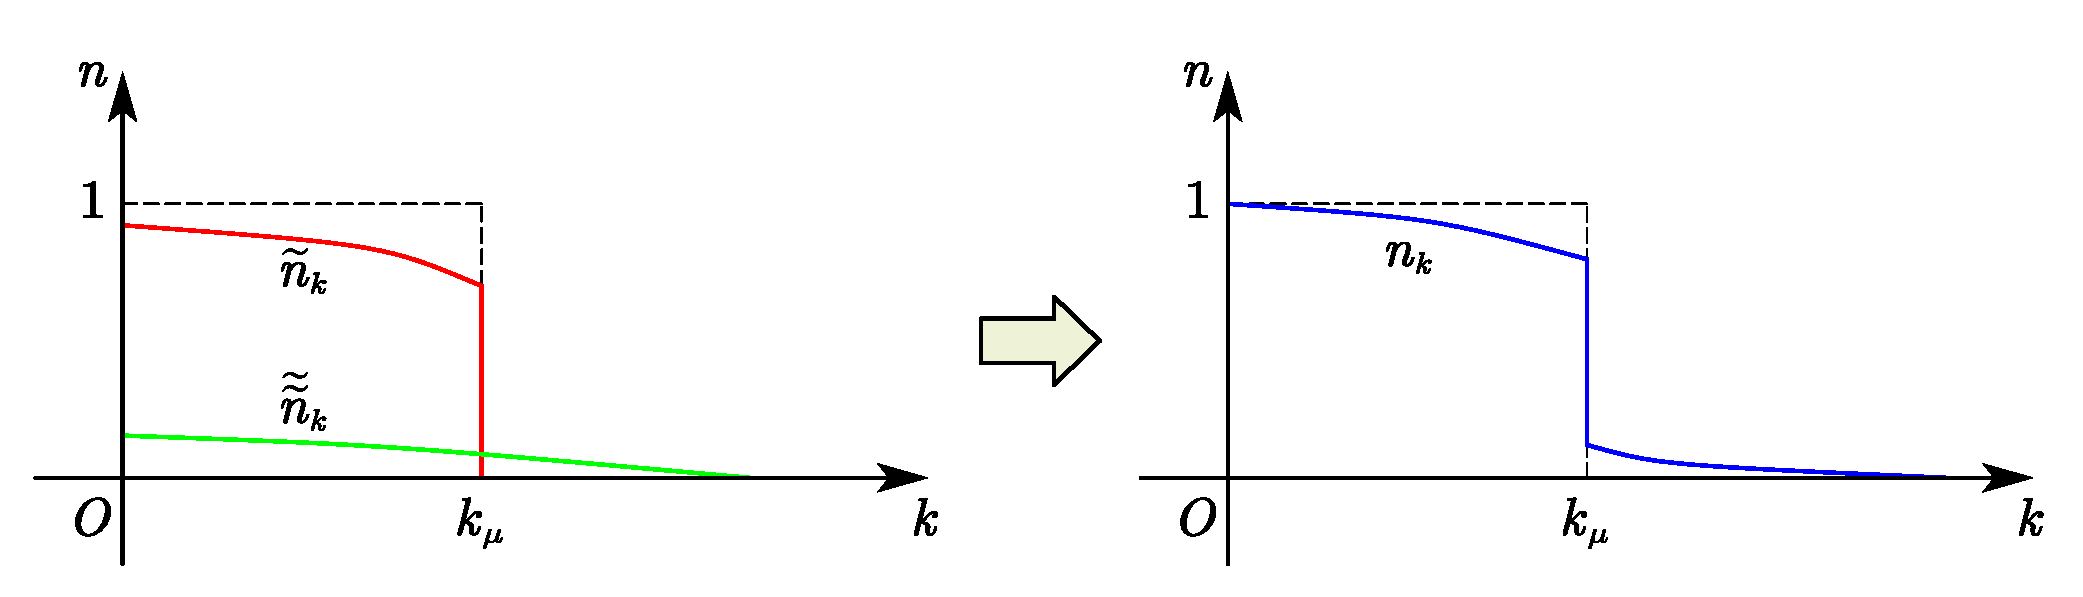
\includegraphics[width=15cm]{figure/dist.pdf}
    \caption{最强发散项近似下的基态电子分布函数示意图.}
    \label{MD-nk}
\end{figure}

凝胶模型的最强发散项近似能够反映系统的等离振荡. 但进一步考虑该模型电子关联, 需要利用密度关联格林函数, 得到介电函数的零点, 即格林函数的极点. 下面利用费曼图对这一方法进行讨论.
\subsection{密度关联格林函数}
回顾前面得到的, 电子间严格的有效相互作用的费曼图是 
\begin{equation}
    \feyndiagram{\propag[doublefermion, dashed] (1,0) to (-1,0);}=
    \feyndiagram{\propag[chasca] (1,0) to (-1,0);}
    +\feyndiagram{
        \normalpolar{a}{0,0};
            \propag[chasca](a) to (-1.5,0);
            \propag[doublefermion, dashed] (1.5,0) to (a);
    },
\end{equation}
对应的表达式: 
\begin{equation}
    \tilde{U}(k)=\frac{U(k)}{1-U(k)\Pi^{*}(k)}=\frac{V(\vct{k})}{1-V(\vct{k})\Pi^{*}(k)},
\end{equation}

严格的总极化图展开式为
\begin{equation}
    \singlepolar=\;
    \singlenormalpolar
    +
    \feyndiagram{
        \normalpolar{a}{-1,0};
        \polar{b}{0.5,0};
        \propag[sca] (a) to (b);
    },
\end{equation}
对应的表达式为 
\begin{equation}
    \Pi(k)=\frac{\Pi^*(k)}{1-U(k)\Pi^*(k)}=\frac{\Pi^*(k)}{1-V(\vct{k})\Pi^*(k)}.
\end{equation}

最强发散项近似的有效相互作用表达式为
\begin{equation}
    \feyndiagram{\propag[doublefermion, dashed] (1,0) to (-1,0);}=
    \feyndiagram{\propag[chasca] (1,0) to (-1,0);}
        +
        \feyndiagram{
            \vertex[ringblob] (a) at (0,0){};
            \propag[chasca](a) to (-1.5,0);
            \propag[doublefermion, dashed] (1.5,0) to (a);
        }.
\end{equation}
对应的数学表达式为 
\begin{equation}
    \tilde{U}_{\fun{MD}}(k)=\frac{U(k)}{1-U(k)\Pi^{*(0)}(k)}=\frac{V(\vct{k})}{1-V(\vct{k})\Pi^{*(0)}(k)}.
\end{equation}
在这一近似下, 极化图展开为
\begin{equation}
    \singlepolar=\;
    \feyndiagram{\vertex[ringblob]at(0,0){};}
    +
    \feyndiagram{
        \vertex[ringblob](a)at(-1,0){};
        \polar{b}{0.5,0};
        \propag[sca] (a) to (b);
    },
\end{equation}
对应的表达式为 
\begin{equation}
    \Pi_{\fun{MD}}(k)=\frac{\Pi^{*(0)}(k)}{1-U(k)\Pi^{*(0)}(k)}=\frac{\Pi^{*(0)}(k)}{1-V(\vct{k})\Pi^{*(0)}(k)}.
\end{equation}
总极化 $\Pi_{\fun{MD}}(k)$ 对应着(因果)密度关联格林函数, $\Pi^{*(0)}$ 是 Lindhard 函数. 这一形式可以得出与上一章相同的结果. 

有效相互作用可以进一步改写成 
\begin{equation}
    \tilde{U}(k)\equiv \frac{U(k)}{\epsilon(k)}=\frac{V(\vct{k})}{\epsilon(k)},
\end{equation}
其中有 
\begin{equation}
    \epsilon(k)=1-V(\vct{k})\Pi^*(k)
\end{equation}
称为系统介电函数. 最强发散项近似下有 
\begin{equation}
    \epsilon_{\fun{MD}}(k)=1-V(\vct{k})\Pi^{*(0)}(k).
\end{equation}
于是有一般成立的关系式:
\begin{equation}
    \frac{1}{\epsilon(k)}=1+V(\vct{k})\Pi(k)\Rightarrow \frac{1}{\epsilon_{\fun{MD}}(k)}=1+V(\vct{k})\Pi_{\fun{MD}}(k).
\end{equation}
下面具体计算在几种极限下的 Lindhard 函数.

(A) 长波极限($q\to 0$).

根据之前的计算, 得到 
  \begin{align}
        \Pi^{*(0)}(\vct{q},\omega)=&2\int\frac{\dd\vct{k}}{(2\pi)^3}\theta(|\vct{k}+\vct{q}|-k_{\fun{F}})\theta(k_{\fun{F}}-|\vct{k}|)\nonumber\\
        &\times \lmi \frac{1}{\omega-\omega_{kq}+\ii\eta}-\frac{1}{\omega+\omega_{kq}-\ii\eta} \rmi,
    \end{align}
其中 
\begin{equation}
    \omega_{kq}\equiv \epsilon_{k+q}^0-\epsilon_k^0=\frac{1}{2m}\ls q^2+2\vct{q}\cdot \vct{k} \rs.
\end{equation}
采用球极坐标
$$
\begin{tikzpicture}
    \draw [arrows = {-Stealth[reversed,reversed]}] (0,0) -- (2,0);
    \draw [arrows = {-Stealth[reversed,reversed]}] (0,0) -- (0,2);
    \draw [arrows = {-Stealth[reversed,reversed]}] (0,0) -- (-1.4,-1);
    \draw [arrows = {-Stealth[harpoon]}] (-0.3,1) -- (-0.3,1.7);
    \draw (-0.6,1.7) node{$\vct{q}$};
    \draw (2.3,0) node{$k_y$};
    \draw (0,2.3) node{$k_z$};% node和文字大括号之间不要加空格.
    \draw (-1.5,-1.4) node{$k_x$};
    \draw (-0.1,-0.3) node{$O$};
    \draw [very thick, arrows = {-Stealth[reversed,reversed]}] (0,0) -- (1,1.4);
    \draw [line width =1pt, dashed] (1,1.4) -- (1,-1.3);
    \draw [line width =1pt, dashed] (1,-1.3) -- (0,0);
    \draw (1.2,1.6) node{$\vct{k}$};
    \draw [-Stealth] (0,1) arc [start angle=90, end angle=40, radius=20pt];
    \draw [-Stealth] (-0.7,-0.5) arc [start angle=-120, end angle=-69, radius=40pt];
    \draw (0.3,1.3) node{$\theta$};
    \draw (0,-1) node{$\varphi$};
\end{tikzpicture}
$$
Lindhard 函数进一步写成 
  \begin{align}
        \Pi^{*(0)}(\vct{q},\omega)=&\frac{2}{(2\pi)^3}\int_0^{2\pi}\dd\varphi\int_0^\pi\sin\theta\dd\theta\int_{|\vct{k}|\le k_{\fun{F}},\atop |\vct{k}+\vct{q}|>k_{\fun{F}}}k^2 \dd k\nonumber\\
        &\times\lmi \frac{1}{\omega-\frac{1}{2m}\ls q^2+2kq\cos\theta \rs+\ii\eta}-\frac{1}{\omega+\frac{1}{2m}(q^2+2kq\cos\theta)-\ii\eta} \rmi,
    \end{align}
在长波极限下, $\vct{q}$ 取值很小, 相应有 $\vct{k}\to \vct{k}_{\fun{F}}$. 取极限 $k\to k_{\fun{F}}$, $q$ 只保留到一次项, $q^2=0$. 于是积分与 $k$ 无关. 利用对 $k$ 的限制:
\begin{itemize}
    \item $k\le k_{\fun{F}}$,
    \item $\sqrt{k^2+q^2+2qk\cos\theta}>k_{\fun{F}}\Rightarrow k+q\cos\theta>k_{\fun{F}}\Rightarrow\cos\theta>0$,
    \item $k>k_{\fun{F}}-q\cos\theta$,
\end{itemize} 
积分式可以写成 
 \begin{align}
        \Pi^{*(0)}(\vct{q},\omega)=&\frac{1}{2\pi^2}\int_0^{\pi/2}\sin\theta\dd\theta \int_{k_{\fun{F}}-q\cos\theta}^{k_{\fun{F}}}k_{\fun{F}}^2\dd k\nonumber\\
        &\times \lmi \frac{1}{\omega-\frac{1}{2m}\ls 2k_{\fun{F}}q\cos\theta \rs+\ii\eta} -\frac{1}{\omega+\frac{1}{2m}(2k_\fun{F}q\cos\theta)-\ii\eta}\rmi,
    \end{align}
令 $x=\cos\theta$, 有 
 \begin{align}
        \Pi^{*(0)}(\vct{q},\omega)=&\frac{q k_{\fun{F}}^2}{2\pi^2}\int_0^1\dd x\; x\nonumber\\
        &\times\lmi \frac{1}{\omega-\frac{k_{\fun{F}}qx}{m}+\ii\eta}-\frac{1}{\omega+\frac{k_{\fun{F}}qx}{m}-\ii\eta} \rmi,
    \end{align}
再引入 $\displaystyle\xi\equiv \frac{m\omega}{k_{\fun{F}}q}$, 得到 
\begin{equation}
    \Pi^{*(0)}(\vct{q},\omega)=\frac{mk_{\fun{F}}}{2\pi^2}\int_0^1 \dd x\; x\lmi \frac{1}{\xi-x+\ii\eta}-\frac{1}{\xi+x-\ii\eta} \rmi.
\end{equation}
利用柯西主值积分, 第一项: 
  \begin{align}
        \int_0^1\dd x\; x\frac{1}{\xi-x+\ii\eta}=&\int_0^1\dd x\; x\lmi \frac{\mathcal{P}}{\xi-x}-\ii\pi\delta(\xi-x) \rmi\nonumber\\
        =&\mathcal{P}\int_0^1\dd x\frac{x-\xi+\xi}{\xi-x}-\ii\pi\xi\theta(1-\xi)\theta(\xi)\nonumber\\
        =&-1-\xi\mathcal{P}\int_0^1\frac{\dd x}{x-\xi}-\ii\pi\xi\theta(1-\xi)\theta(\xi),
    \end{align}
其中, 当 $0<\xi<1$ 时, 有 
\begin{equation}
    \mathcal{P}\int_0^1\frac{\dd x}{x-\xi}=\int_0^{\xi-\delta}\frac{\dd x}{x-\xi}+\int_{\xi+\delta}^1\frac{\dd x}{x-\xi}=\ln \left| \frac{1-\xi}{\xi} \right|.
\end{equation}
代回第一项积分, 有 
\begin{equation}
    \int_0^1\dd x\frac{x}{\xi-x+\ii\eta}=-1-\xi\ln\left| \frac{1-\xi}{\xi} \right|-\ii\pi\xi\theta(1-\xi),\quad (0<\xi<1).
\end{equation}
类似地, 有第二项
 \begin{align}
        -\int_0^1\dd x\frac{x}{\xi+x-\ii\eta}=&-1+\xi\ln\left| \frac{1+\xi}{\xi} \right|+\ii\pi\xi\theta(1+\xi),\quad (-1<\xi<0)\nonumber\\
        =&-1+\xi\ln\left| \frac{1+\xi}{\xi} \right|-\ii\pi|\xi|\theta(1-|\xi|).
    \end{align}
两项合并, 得到 
\begin{equation}
    \int_0^1\dd x\;x\lmi \frac{1}{\xi-x+\ii\eta}-\frac{1}{\xi+x-\ii\eta} \rmi=-2+\xi\ln\left| \frac{1+\xi}{1-\xi} \right|-\ii\pi\theta(1-|\xi|)|\xi|.
\end{equation}
代回 Lindhard 函数中, 有 
\begin{equation}
    \Pi^{*(0)}(\vct{q},\omega)=\frac{-mk_{\fun{F}}}{\pi^2}\lmi 1-\frac{\xi}{2}\ln\left| \frac{1+\xi}{1-\xi} \right|+\frac{\ii\pi}{2}|\xi|\theta(1-|\xi|) \rmi,
\end{equation}
其中有 $\displaystyle \xi\equiv \frac{m\omega}{k_{\fun{F}}q}$, $q\to 0$, $\xi\to \infty$. 考虑小量展开 
\begin{equation}
    \ln\left| \frac{1+\xi}{1-\xi} \right|\approx \frac{2}{\xi}+\frac{2}{3}\frac{1}{\xi^3},
\end{equation}
有 
\begin{equation}
    \Pi^{*(0)}(\vct{q}\to 0,\omega)=\frac{mk_{\fun{F}}}{\pi^2}\frac{1}{3}\ls \frac{k_{\fun{F}}q}{m\omega} \rs^2=\frac{nq^2}{m\omega^2},\quad n=\frac{N}{V}.
\end{equation}
总极化的表达式 
\begin{equation}
    \Pi_{\fun{MD}}(\vct{q},\omega)=\frac{\Pi^{*(0)}(\vct{q},\omega)}{1-V(\vct{q})\Pi^{*(0)}(\vct{q},\omega)},
\end{equation}
等离激元的振荡频率由上式的极点方程给出, 即 
 \begin{align}
        1=&V(\vct{q})\Pi^{*(0)}(\vct{q},\omega),\nonumber\\
        \Rightarrow 1=&\frac{4\pi e^2}{q^2}\frac{nq^2}{m\omega^2},\nonumber\\
        \Rightarrow \omega^2=&\frac{4\pi e^2n}{m}= \omega_p^2,\nonumber\\
        \Rightarrow\omega_p=&\sqrt{\frac{4\pi e^2n}{m}},
    \end{align}
即得等离振荡频率, 也就是系统集体激发的准粒子能谱. 

(B) 静电屏蔽($\omega=0$).

Lindhard 函数: 
 \begin{align}
        \Pi^{*(0)}=&-4\int\frac{\dd\vct{k}}{(2\pi)^3}\frac{\theta(|\vct{k}+\vct{q}|-k_{\fun{F}})\theta(k_{\fun{F}}-|\vct{k}|)}{\epsilon_{k+q}^0-\epsilon_k^0}\nonumber\\
        =&-4\int\frac{\dd \vct{k}}{(2\pi)^3}\frac{[1-\theta(k_{\fun{F}}-|\vct{k}+\vct{q}|)]\theta(k_{\fun{F}}-|\vct{k}|)}{\epsilon_{k+q}^0-\epsilon_k^0},
    \end{align}
其中, 虚部始终为零. 考虑括号中第二项: 
\begin{equation}
        A=4\int\frac{\dd\vct{k}}{(2\pi)^3}\frac{\theta(k_{\fun{F}}-|\vct{k}+\vct{q}|)\theta(k_{\fun{F}}-|\vct{k}|)}{\epsilon_{k+q}^0-\epsilon_k^0},
\end{equation}
作变量代换, 有 $\vct{k}\to -\vct{k}-\vct{q}$, 得到 
\begin{equation}
    A=4\int\frac{\dd\vct k}{(2\pi)^3}\frac{\theta(k_{\fun{F}}-|\vct{k}|)\theta(k_{\fun{F}}-|\vct{k}+\vct{q}|)}{\epsilon_k^0-\epsilon_{k+q}^0},
\end{equation}
这里得到的结果, 分子不变, 分母差一负号, 即有 $A=-A\Rightarrow A=0$. 于是 $\Pi^{*(0)}$ 表达式中只需要考虑第一项. 有:
\begin{align}
        \Pi^{*(0)}(\vct{q},0)=&-4\int\frac{\dd \vct{k}}{(2\pi)^3}\frac{\theta(k_{\fun{F}}-|\vct{k}|)}{\frac{1}{2m}(q^2+2\vct{q}\cdot \vct{k})}\nonumber\\
        =&-\frac{2m}{\pi^2}\int_0^{k_{\fun{F}}}k^2\dd k\int_{-1}^1\frac{\dd x}{q^2+2qkx}\nonumber\\
        =&-\frac{m}{\pi^2 q}\int_0^{k_{\fun{F}}}k\dd k\ln\left| \frac{q^2+2qk}{q^2-2qk} \right|,
    \end{align}
其中第二步取 $x\equiv \cos\theta$. 再利用积分公式 
\begin{equation}
    \int\dd x x\ln|x+a|=\frac{1}{2}(x^2-a^2)\ln|x+a|-\frac{x^2}{4}+\frac{ax}{2},
\end{equation}
表达式进一步写成 
\begin{equation}
    \Pi^{*(0)}(\vct{q},0)=-\frac{mk_{\fun{F}}}{2\pi^2}\lmi 1+\frac{1}{y}\ls 1-\frac{y^2}{4} \rs\ln\left| \frac{1+\frac{y}{2}}{1-\frac{y}{2}} \right| \rmi,
\end{equation}
其中有 $y\equiv q/k_{\fun{F}}$. 下面利用这一结果来讨论系统的有效相互作用.
 \begin{align}
        \tilde U_{\fun{MD}}(\vct{q},0)=&\frac{V(\vct{q})}{1-V(\vct{q})\Pi^{*(0)}(\vct{q},0)}\nonumber\\
        =&\frac{V(\vct{q})}{\epsilon_{\fun{MD}}(\vct{q},0)}\nonumber\\
        =&\frac{4\pi e^2}{q^2-4\pi e^2\Pi^{*(0)}(\vct{q},0)},
    \end{align}
傅里叶变换到实空间下, 有 
\begin{equation}
    \tilde U_{\fun{MD}}(\vct{r})=\int\frac{\dd\vct{q}}{(2\pi)^3}\tilde U_{\fun{MD}}(\vct{q},0)\e^{\ii\vct{q}\cdot \vct{r}}\propto \frac{\cos(2k_{\fun{F}}r)}{r^3},
\end{equation}
在 $r\to \infty$ 时振荡衰减. 这一结果常称为 Friedel 震荡, 如图\ref{friedel}所示. 

\begin{figure}[htbp]
    \centering
    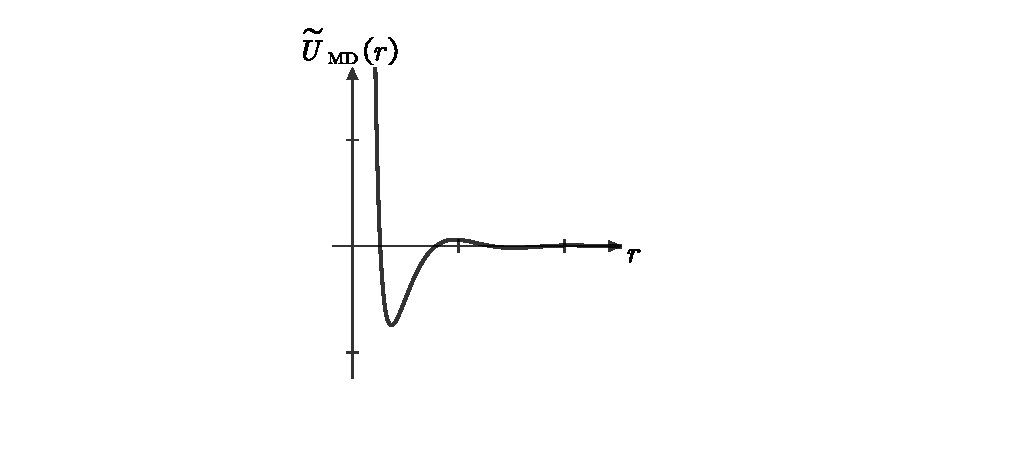
\includegraphics[width=4cm]{figure/friedel.pdf}
    \caption{Friedel 震荡函数.}
    \label{friedel}
\end{figure}

下面讨论 $q\to 0,\omega\to 0$ 的情况: 
\begin{equation}
    \Pi^{*(0)}(\vct{q}\to 0,0)=-\frac{mk_{\fun{F}}}{\pi^2},
\end{equation}
\begin{equation}
    \tilde U_{\fun{MD}}(\vct q\to 0,0)=\frac{4\pi e^2}{q^2+4\pi e^2\frac{mk_{\fun{F}}}{\pi^2}}=\frac{4\pi e^2}{q^2+\lambda^2},
\end{equation}
其中有 
\begin{equation}
    \lambda^2\equiv \frac{4 e^2mk_{\fun{F}}}{\pi}=\frac{6\pi ne^2}{E_{\fun{F}}},\quad n=\frac{N}{V},
\end{equation}
我们称 
\begin{equation}
    \lambda^{-1}=\frac{1}{\sqrt{\frac{6\pi ne^2}{E_{\fun{F}}}}}
\end{equation}
为 Thomas-Fermi 屏蔽长度. 并有 
\begin{equation}
    \tilde{U}_{\fun{MD}}(\vct{r})=\frac{e^2}{r}\e^{-\lambda r}
\end{equation}
称为汤川(Yukawa)屏蔽势, 如图\ref{yukawa}所示.
\begin{figure}[htbp]
    \centering
    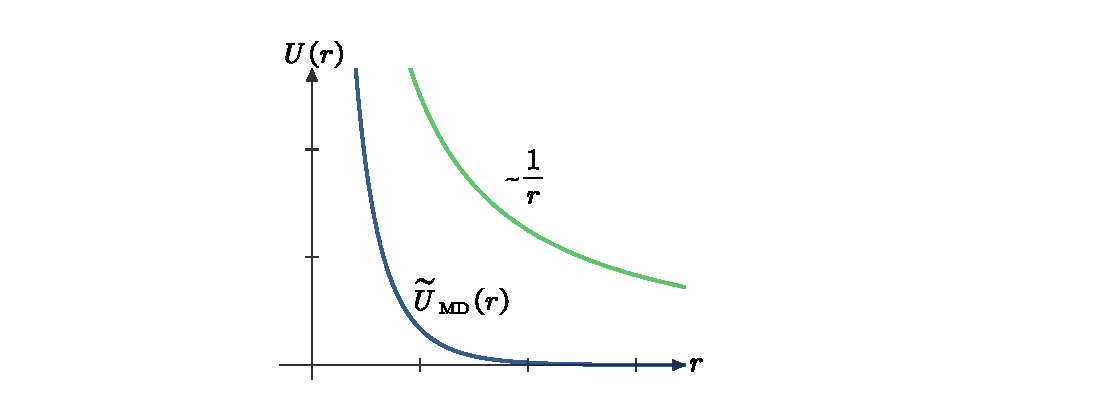
\includegraphics[width=5cm]{figure/yukawa.pdf}
    \caption{汤川屏蔽势和库仑势.}
    \label{yukawa}
\end{figure}
\begin{note}
    下面讨论一下最强发散项近似的成立条件.

    考虑这样三种自能图:
    $$
        \feyndiagram{
            \vertex(a)at(-1,-1);
            \vertex(b)at(1,-1);
            \vertex(c)at(-1,1);
            \vertex(d)at(1,1);
            \propag[plain](a)to(b);
            \propag[sca](a)to(c);
            \propag[sca](b)to(d);
            \propag[plain](c)to[half left, looseness=1.5](d);
            \propag[plain](d)to[half left, looseness=1.5](c);
            \vertex(e)at(-1.3,0){$\vct{q}$};
            \vertex(f)at(1.3,0){$\vct{q}$};
        },\quad
        \feyndiagram{
            \vertex(a)at(-1,-1);
            \vertex(b)at(1,-1);
            \vertex(c)at(-1,1);
            \vertex(d)at(1,1);
            \propag[plain](a)to(b);
            \propag[sca](a)to(c);
            \propag[sca](b)to(d);
            \propag[plain](c)to[half left, looseness=1.5](d);
            \propag[plain](d)to[half left, looseness=1.5](c);
            \vertex(e)at(-1.3,0){$\vct{q}$};
            \vertex(f)at(1.3,0){$\vct{q}$};
            \propag[sca](0,1.8)to(0,0.1);
        },\quad
        \feyndiagram{
            \vertex(a)at(-1,-1);
            \vertex(b)at(1,-1);
            \vertex(c)at(-1,1);
            \vertex(d)at(1,1);
            \propag[plain](a)to(b);
            \propag[sca](a)to(c);
            \propag[sca](b)to(d);
            \propag[plain](c)to[half left, looseness=1.5](d);
            \propag[plain](d)to[half left, looseness=1.5](c);
            \vertex(e)at(-1.3,0){$\vct{q}$};
            \vertex(f)at(1.3,0){$\vct{q}$};
            \propag[sca](-0.4,1.7)to(-0.4,0.3);
            \propag[sca](0.4,1.7)to(0.4,0.3);
        },\quad
    $$
    这三种图的发散程度相同, 但我们在取近似时, 只考虑了第一种, 而忽略了后两种. 这是因为在高密度情况下, 第一项的贡献要远大于其它项. 下面证明这一结论.

    在高密度近似下, 假设一个电子所占据的体积可以用等体积的球来描述, 即有 
    \begin{equation}
        \frac{V}{N}\equiv \frac{4}{3}\pi r^3_0.
    \end{equation}
    引入无量纲参数 $r_s$, 令 $r_0\equiv r_sa_H$, 其中 $a_H$ 是氢原子玻尔第一轨道半径, 有 $a_H=\hbar^2/me^2$.
    高密度近似对应着 $r_s\ll 1$, 即 
    \begin{equation}
        r_s=\frac{\ls \frac{9}{4}\pi \rs^{1/3}}{a_Hk_{\fun{F}}}\ll 1\Rightarrow \frac{1}{a_Hk_{\fun{F}}}\ll 1.
    \end{equation}
    下面主要分析 $\feyndiagram{\vertex[ringblob](0,0){};}$ 和 $\feyndiagram{\propag[plain](-0.4,0)to[half left, looseness=1.8](0.4,0);\propag[plain](0.4,0)to[half left, looseness=1.8](-0.4,0);\propag[sca](0,-0.4)to(0,0.4);}$ 的贡献.

    (a)
    $$
    \feyndiagram{
        \vertex(c)at(-1,0);
        \vertex(d)at(1,0);
        \propag[fer](c)to[half left, looseness=1.5](d);
        \propag[fer](d)to[half left, looseness=1.5](c);
        \vertex(a)at(0,-1.3){$\vct{k}+\vct{k}_1$};
        \vertex(v)at(0,1.3){$\vct{k}_1$};
    }
    $$
    \begin{equation}
        \Pi^{*(0)}(k)=-2\ii\int\frac{\dd k_1}{(2\pi)^4}G^0(k+k_1)G^0(k_1).
    \end{equation}

    (b)
    $$
    \feyndiagram{
        \vertex(a)at(-1,0);
        \vertex(b)at(1,0);
        \vertex(c)at(0,1);
        \vertex(d)at(0,-1);
        \propag[fer](a)to[quarter left, looseness=1](c);
        \propag[fer](c)to[quarter left, looseness=1](b);
        \propag[fer](b)to[quarter left, looseness=1](d);
        \propag[fer](d)to[quarter left, looseness=1](a);
        \propag[sca](c)to(d);
        \vertex (1) at (-1,-1.2){$\vct{k}_2+\vct{k}$};
        \vertex (2) at (-1,1.2){$\vct{k}_2$};
        \vertex (3) at (1,1.2){$\vct{k}_1$};
        \vertex (4) at (1,-1.2){$\vct{k}_1+\vct{k}$};
        \vertex (5) at (-0.2,0){$\vct{k}_2-\vct{k}_1$};
    }
    $$
      \begin{align}
            \Pi^{*(1)}(k)=&-2\ii^2\int\frac{\dd k_1}{(2\pi)^4}\int\frac{\dd k_2}{(2\pi)^4}G^0(k_1+k)G^0(k_1) V(\vct{k}_1-\vct{k}_2)G^0(k_2+k)G^0(k_2)\nonumber\\
            =&-2\ii^2\frac{4\pi e^2}{k_{\fun{F}}^2}\lmi \int\frac{\dd k_1}{(2\pi)^4}G^0(k_1+k)G^0(k_1) \rmi\lmi \int\frac{\dd k_2}{(2\pi)^4}G^0(k_2+k)G^0(k_2) \rmi,
        \end{align}
    可以看出, 两个表达式的关系为 
    \begin{equation}
        \left| \Pi^{*(1)}(k) \right|\sim\frac{e^2}{k_{\fun{F}}^2}\left| \Pi^{*(0)}(k) \right|^2,
    \end{equation}
    考虑两个函数的比值, 有 
    \begin{equation}
        \frac{\left| \Pi^{*(1)}(k) \right|}{\left| \Pi^{*(0)}(k) \right|}\sim\frac{e^2}{k_{\fun{F}}^2}\left| \Pi^{*(0)}(k) \right|\sim\frac{e^2}{k_{\fun{F}}^2}mk_{\fun{F}}=\frac{me^2}{k_{\fun{F}}}\sim\frac{1}{k_{\fun{F}}a_H}.
    \end{equation}
    上式在高密度极限下远小于 1. 于是有 $|\Pi^{*(1)}(k)|\ll |\Pi^{*(0)}(k)|$ 可以忽略, 对应着电子的无规则相位最强. 这是近似成立的条件.
\end{note}
\begin{question}{}{}
    计算下面两个动量空间费曼图, 要求对所有内部自旋求和, 所有内部频率积分.
    $$
        \feyndiagram{
            \propag[plain](-2,0) to (2,0);
            \propag[plain](-1,1.5) to[half left, looseness=1.5](1,1.5);
            \propag[plain](1,1.5) to[half left, looseness=1.5](-1,1.5);
            \propag[sca](0,0)to(0,0.6);
            \propag[sca](-1,0) to (-1,1.5);
            \propag[sca](1,0)to(1,1.5);
        }
        \qquad
        \feyndiagram{
            \propag[plain](-2,0) to (2,0);
            \propag[sca](-1.5,0)to[half left, looseness=1.6](0.5,0);
            \propag[sca](-0.5,0) to[half left, looseness=1.6](1.5,0);
        }
    $$
\end{question}